\documentclass{article}

\usepackage{amsmath,amsfonts,amssymb,amsthm}
\usepackage{enumitem}
\usepackage{a4wide}
\usepackage[document]{ragged2e}
\usepackage{tikz}
\usepackage[utf8]{inputenc}
\usepackage[T1]{fontenc}
\usepackage[german]{babel}
\usepackage{hyphenat}
\usepackage{listings}
\usepackage{caption}
\usepackage{imakeidx}
\usepackage{wasysym}
\usepackage{color}
\usepackage{graphicx}
\usepackage{accents}
\usepackage{stmaryrd}
\usepackage{pgfplots}
\usepackage{varwidth}
\usepackage{mathtools}



\usetikzlibrary{positioning, calc}
\usetikzlibrary{decorations.pathreplacing,angles,quotes}
\usetikzlibrary{decorations.pathmorphing,snakes}
\usetikzlibrary{shapes.misc}
\usetikzlibrary{intersections,through,backgrounds}
\usetikzlibrary{matrix}
\usetikzlibrary{arrows}



\theoremstyle{plain}
\newtheorem{theorem}{Theorem}
\newtheorem{lemma}[theorem]{Lemma}
\newtheorem*{lemma*}{Lemma}
\newtheorem{cor}[theorem]{Korollar}
\newtheorem*{cor*}{Korollar}
\newtheorem{prop}[theorem]{Proposition}
\setlength{\parskip}{1em}

\theoremstyle{definition}
\newtheorem{definition}[theorem]{Definition}
\newtheorem*{definition*}{Definition}
\newtheorem{notation}[theorem]{Notation}
\newtheorem{bemerkung}[theorem]{Bemerkung}
\newtheorem*{bemerkung*}{Bemerkung}
\newtheorem{bsp}[theorem]{Beispiel}
\newtheorem*{remark*}{remark}
\newtheorem{remark}{remark}

\numberwithin{equation}{section}

\newcommand{\norm}[1] {
\left|\left| #1 \right|\right|
}

\newcommand{\hnorm}[1] {
\left|\left|\left| #1 \right|\right|\right|
}

\newcommand{\colvec}[1]{
\begin{pmatrix}#1\end{pmatrix}
}

\newcommand{\vect}[1]{
\begin{pmatrix}#1\end{pmatrix}
}

\newcommand{\skprod}[2]{
\left \langle #1,#2 \right \rangle
}
\newcommand{\abs}[1] {
\left| #1 \right|
}

\newcommand{\br}[1] {
\left( #1 \right)
}

\newcommand{\R}[0] {
\mathbb R
}

\newcommand{\Z}[0] {
    \mathbb Z
}

\newcommand{\N}[0] {
    \mathbb N
}

\newcommand{\F}[0]{
    \mathcal F
}

\newcommand{\srmatrix}[1] {
\left( \begin{smallmatrix} #1 \end{smallmatrix} \right)
}

\newcommand{\mtitle}[1] {
    \begin{center}
        \large{\textbf{#1}}
    \end{center}
}

\newcommand{\Index}[1]{#1\index{#1}}

\newcommand{\mim}[1] {
\underline{\textbf{#1\index{#1}}}
}

\newcommand{\C}[0]{
    \cdot
}

\newcommand{\pa}[1] {
    \par{\textbf{#1}}
}

\newcommand{\tvmark}[3] {
    \draw[] (#1,0.1+#2) -- (#1,-0.1+#2) node[anchor =north] {\small #3};
}
\newcommand{\thmark}[3] {
    \draw[] (#1+0.1,#2) -- (#1-0.1,#2) node[left] {\small #3};
}

\newcommand{\tvnmark}[3] {
    \draw[] (#1,#2-0.1) node[below] {\small #3};
}

\newcommand{\tlbar}[5]{
    \draw[thick] (#1,#2-0.1) node[below] {\small #4} -- (#1,#3) node[above] {#5};
    \draw[thick] (#1-0.1,#3) -- (#1+0.1,#3);
}

\newcommand{\filter}[1] {
\begin{tabular}{|c|c|c|}
    \hline
    #1\\
    \hline
\end{tabular}
}
\newcommand{\quo}[1] {
\glqq #1 \grqq
}

\newcommand{\x}[0] {
  \boldsymbol{x}
}
\newcommand{\y}[0] {
    \boldsymbol{y}
}

\newcommand{\mat}[1] {
\begin{pmatrix} #1 \end{pmatrix}
}

\definecolor{dkgreen}{rgb}{0,0.6,0}
\definecolor{gray}{rgb}{0.5,0.5,0.5}
\definecolor{mauve}{rgb}{0.58,0,0.82}

\lstset{frame=tb,
language=Matlab,
aboveskip=10mm,
belowskip=10mm,
showstringspaces=false,
columns=flexible,
basicstyle={\small\ttfamily},
numbers=left,
identifierstyle=\color{black},
numberstyle=\small\color{gray},
keywordstyle=\color{blue},
commentstyle=\color{dkgreen},
stringstyle=\color{mauve},
breaklines=true,
breakatwhitespace=true,
tabsize=3}

%Font
%\usepackage{tgadventor}
\renewcommand*\rmdefault{cmss}
\makeindex

\begin{document}
\title{Mathematische Bildverarbeitung}
%\author{Jonas Sattler}
\date{}
\maketitle

\tableofcontents

\newpage

\section{Überblick}
    \subsection{Techniken der Bildverarbeitung}
        \begin{enumerate}[label=\textbullet]
            \item Kontrastverbesserung
            \item Entrauschen
            \item Kantendetektion
            \item Schärfen
            \item Inpainting
            \item Segmentierung (Einzelne Objekte detektieren)
            \item Registrierung (Bilder des selben Objektes in Einklang bringen)
        \end{enumerate}

    \subsection{Unser Fokus}
        \begin{enumerate}[label=\textbullet]
            \item Mathematische Beschreibung
        \end{enumerate}

    \subsection{Verwandte Vorlesungen}
        \begin{enumerate}[label=\textbullet]
            \item 3D Computervision
            \item Digitale Bildanalyse
            \item Mustererkennung und Datenkompression
            \item Medical imaging
        \end{enumerate}

    \subsection{Literatur}
        \begin{enumerate}[label=\textbullet]
            \item Bredies, Lorenz : Mathematische Bildverarbeitung
            \item Aubert, Kornprobst : Mathematical Problems in Image Processing
            \item Modersitzki : Numerical Methods for Image Registration
            \item Alt : Lineare Funktionalanalysis
        \end{enumerate}

\section{Was ist ein Bild?}
    \subsection{Definition}
        \begin{minipage}[t]{0.45\linewidth}
            \mtitle{\underline{Digitale/diskrete Sicht}}
            \begin{center}
                \begin{tikzpicture}
                    \fill[black!30!white] (1,2) rectangle (1.5,2.5);
                    \draw[step=0.5,thin,draw=black] (0,0) grid (4,4);
                    \draw[thick] (0,0) rectangle (4,4);
                \end{tikzpicture}
                \captionof{figure}{Diskretes Bild}
                Darstellung als Matrix.
            \end{center}
        \end{minipage}
        \hfill\vrule\hfill
        \begin{minipage}[t]{0.45\linewidth}
            \mtitle{\underline{Kontinuierlich/analoge Sicht}}
            \begin{center}
                \begin{tikzpicture}
                    \draw[thick,->] (0,0) -- (3,0) node[anchor=west] {X};
                    \draw[thick,->] (0,0) -- (0,3) node[anchor=south] {Y};
                    \draw[thick] (0.2,0.2) rectangle (2.8,2.8);
                    \draw (1.5,2) node[] {\tiny{\textbullet}} node[anchor=west] {\small$(x,y)$};
                    \draw[] (1.5,0.1) -- node[anchor=north] {\small x} (1.5,-0.1);
                    \draw[] (0.1,2) -- node[anchor=east] {\small y} (-0.1,2);
                    \draw[|-|] (0.2,-0.4) node[anchor=north] {\small a} -- (2.8,-0.4) node[anchor=north] {\small b};
                    \draw[|-|] (-0.4,0.2) node[anchor=east] {\small c} -- (-0.4,2.8) node[anchor=east] {\small d};
                \end{tikzpicture}
                \captionof{figure}{Kontinuierliches Bild}
                Darstelllung als Funktion in zwei Veränderlichen
            \end{center}
        \end{minipage}

        \ \\

        \begin{minipage}[t]{0.47\linewidth}
            \pa{Werkzeuge:} Lineare Algebra
            \pa{Vorteile:} Endlicher Speicher
            \pa{Nachteile:} Probleme bei zoomen und drehen
        \end{minipage}
        \hfill\vrule\hfill
        \begin{minipage}[t]{0.47\linewidth}
            \pa{Werkzeuge:} Analysis
            \pa{Vorteile:} Mehr Freiheit (z.b. Kante=Linie entlang einer Unstetigkeit)
            \pa{Nachteile:} Unendlicher Speicher
        \end{minipage}

        \begin{definition*}
            Ein \mim{Bild} ist eine Funktion $u: \Omega \to F$, wobei $\Omega \subset \mathbb Z^d$ (im diskreten Fall) oder $\Omega \subset \mathbb R^d$ (im kontinuierlichen Fall).
            \begin{enumerate}
                \item[$d=2$:] Typisches 2D Bild
                \item[$d=3$:] 3D-Bild bzw. "Körper" \ \underline{oder} Video: 2D Ort + Zeit
            \end{enumerate}
            F ist der \mim{Farbraum}, Beispiele:
            \begin{enumerate}[label=\textbullet]
                \item F$=[0,1]$ oder F=$\{0,1,..., 255\}$, Graustufen
                \item F$=\{0,1\}$ schwarz/weiß
                \item F$=[0,1]^3$ oder F$=\{0,1,...,255\}^3$ Farbbilder
            \end{enumerate}
        \end{definition*}
    \subsection{Umwandlung}

        \pa{Kontinuierlich $\to$ Diskret:}\\
            \begin{minipage}[t]{0.49\linewidth}
                \
                \begin{center}
                    \begin{tikzpicture}
                        \draw (-0.5,2) node {$\Omega=$};
                        \draw[step=0.5,thin,draw=black,dotted] (0.01,0.01) grid (3.99,3.99);
                        \draw[thick] (0,0) rectangle (4,4);
                        \draw[thick] (2,2) rectangle (2.5,2.5);
                        \draw[] (2.1,2.1) -- (3,-0.3) node[anchor = south west, yshift = -7] {\small Box $B_i$};
                    \end{tikzpicture}
                \end{center}
            \end{minipage}
            \hfill\vrule\hfill
            \begin{minipage}[t]{0.49\linewidth}
                \
                \begin{center}
                    \begin{enumerate}[label=\textbullet]
                        \item $\Omega$ in Gitter zerlegen
                        \item Jede Box durch nur einen Farbwert approximieren
                        \item Etwa durch den Funktionswert im Mittelpunkt der Box
                        \item oder durch den Mittelwert in der Box:\\ $\displaystyle \frac{1}{\abs{B_i}} \C \int_{B_i}u(x)dx$
                    \end{enumerate}
                \end{center}
            \end{minipage}

                \ \\
            \pa{Diskret $\to$ Kontinuierlich:}\\
                \begin{minipage}[t]{0.49\linewidth}
                    \
                    \begin{center}
                        \begin{tikzpicture}
                            \draw (-1,2) node {$\Omega=$};
                            \draw[->] (-0.25,-0.25) -- (-0.25,4.5);
                            \draw[->] (-0.25,-0.25) -- (4.5,-0.25);
                            \draw (-0.35,4) -- (-0.15,4);
                            \draw (-0.35,0) -- (-0.15,0);
                            \draw (0,-0.35) -- (0,-0.15);
                            \draw (4,-0.35) -- (4,-0.15);
                            \draw[step=0.5,thin,draw=black] (0,0) grid (4,4);
                            \foreach \x in {0.25,0.75,..., 3.75}{
                                \foreach \y in {0.25,0.75,..., 3.75}{
                                    \draw (\x,\y) node {\tiny \textbullet};
                            }
                            }
                            \draw[thick] (0,0) rectangle (4,4);
                            \draw[thick] (2,2) rectangle (2.5,2.5);
                            \draw[] (2.1,2.1) -- (3,-0.7) node[anchor = south west, yshift = -7] {\small Box $B_i$};
                        \end{tikzpicture}
                    \end{center}
                \end{minipage}
                \hfill\vrule\hfill
                \begin{minipage}[t]{0.49\linewidth}
                    \
                    \begin{center}
                        \begin{enumerate}
                            \item[1.] Idee: Jeder Punkt der Box $B_i$ erhält den Funktionswert von $B_i$ aus als diskretem Pixel $\Rightarrow$ \mim{Nearest neighbour Interpolation}.
                            \item[2.] Idee: Mittelpunkt von Box $B_i$ erhält den Wert von Pixel $B_i$ sonst wird interpoliert.\\
                            Grauwert $g:=$ Gewichtetes Mittel aus Grauwerten $a,b,c,d$.\\
                        \end{enumerate}

                            \begin{center}
                                \begin{tikzpicture}[scale=1.5]
                                    \draw[step = 1] (0.75,0.75) grid (3.25,3.25);
                                    \foreach \x in {1.5,2.5}{
                                        \foreach \y in {1.5,2.5}{
                                            \draw (\x,\y) node {\tiny \textbullet};
                                    }
                                    }
                                    \draw (1.5,2.5) node[anchor=north west] {a};
                                    \draw (2.5,2.5) node[anchor=south west] {b};
                                    \draw (1.5,1.5) node[anchor=north west] {c};
                                    \draw (2.5,1.5) node[anchor=north west] {d};

                                    \draw (1.5,1.5) rectangle (2.5,2.5);
                                    \draw (1.45,2.15) -- (1.55,2.15);
                                    \draw (1.8,2.45) -- (1.8,2.55);
                                    \draw[decorate,decoration={brace,amplitude=2pt}] (1.5,2.6) -- node[anchor=south] {\small $\alpha$} (1.8,2.6);
                                    \draw[decorate,decoration={brace,amplitude=2pt}] (1.4,2.15) --node[anchor=east] {\small $\beta$} (1.4,2.5);
                                    \draw (1.8,2.15) node {\tiny \textbullet} node[anchor=west, xshift=-2] {\small p};
                                    \draw[decorate,decoration={brace,amplitude=4pt}] (1.5,2.9) -- node[anchor= south west,yshift = 2] {\small 1} (2.5,2.9);
                                    \draw[decorate,decoration={brace,amplitude=4pt}] (1.1,1.5) -- node[anchor= south east, xshift=-2] {\small 1} (1.1,2.5);
                                \end{tikzpicture}
                            \end{center}

                            \small{$g=(1-\alpha) \C (1-\beta) \C a + \alpha \C (1- \beta) \C b + (1-\alpha) \C \beta \C c + \alpha \C \beta \C d$}\\
                            Dieses wird \mim{Bilineare Interpolation} genannt.
                    \end{center}
                \end{minipage}

    \subsection{Beispiel Rotation}
        \begin{center}
            \begin{tikzpicture}%TODO redo
                \draw (0,0.1) -- node[anchor=center] {\tiny \textbullet} node[anchor=north] {\tiny $0$} (3,0.1);
                \draw  (4,0.1) node  {$\overset{\text{\footnotesize um $\alpha$ drehen}}{\Rightarrow}$};
                \draw (6.5,0.1) -- ++(30:1.5);
                \draw (6.5,0.1) node[anchor=center] {\tiny \textbullet} node[anchor=north] {\tiny $0$} -- ++(210:1.5);
                \draw[dotted] (5,0.1) -- (8,0.1);
                \draw (7,0.1) arc[radius=0.5,start angle=0,end angle=30]  node[anchor = north west] {\tiny $\alpha$};
            \end{tikzpicture}
        \end{center}

        \pa{1. Fall, kontinuierliches Bild}\\
            Sei $u$ das alte Bild und $v$ das neue Bild, dann ist die Drehung gegeben durch eine \mim{Drehmatrix}:

            \[D_\varphi \in \R^{d \times d}, D_\varphi=\srmatrix{cos(\varphi) \ -sin(\varphi) \\ sin(\varphi) \ cos(\varphi)}\]

            Damit folgt, dass $D(u)= D_\varphi \Omega$ und $v(x)=u(\underbrace{D_\varphi^{-1}x}_{\in \Omega}) = u(D_{-\varphi}x)$. ($D(u)$ ist die \mim{Domain} von $u$)

        \pa{2. Fall, diskretes Bild}\\
            Dieses ist problematisch, denn I.A. $x \in \Z^d$, aber $D_\varphi x \not \in \Z^d$.

            \begin{center}
                \begin{tikzpicture}
                    \foreach \x in {0,1,2,3}{
                            \draw (0.5*\x,0) node {\tiny \textbullet};
                    }
                    \draw[decorate,decoration={brace,amplitude=4pt,mirror}] (-0.1,-0.1) -- node[anchor= north] {\small $\subset \Z^d$} (1.6,-0.1);
                    \draw[->] (1.75,0) -- (2,0);
                    \draw[step=0.5, shift={(2.25,0.25)}] (0,0) grid (2,-0.5);
                    \foreach \x in {0,1,2,3}{
                        \draw[shift={(2.5,0)}] (0.5*\x,0) node {\tiny \textbullet};
                    }
                    \draw[decorate,decoration={brace,amplitude=4pt,mirror}] (2.15,-0.4) -- node[anchor= north] {\small $\subset \R^d$} (4.35,-0.4);
                    \draw[->] (4.5,0) -- node[above] {\small $D_\varphi$} (4.75,0);
                    \draw[step=0.5, shift={(5,0.25)},rotate around = {45:(1,-0.25)}] (0,0) grid (2,-0.5);
                    \foreach \x in {0,1,2,3}{
                        \draw[shift={(5.25,0)},rotate around = {45:(0.75,0)}] (0.5*\x,0) node {\tiny \textbullet};
                    }
                    \draw[decorate,decoration={brace,amplitude=4pt,mirror}] (4.9,-1) -- node[anchor= north] {\small $\subset \R^d$} (7.1,-1);
                    \draw[->] (7.25,0) -- node[above] {\small rastern} (7.5,0);
                    \draw[->] (4.5,0) -- node[above] {\small $D_\varphi$} (4.75,0);
                    \draw[step=0.5, shift={(8,0.25)},rotate around = {45:(1,-0.25)}] (0,0) grid (2,-0.5);
                    \foreach \x in {0,1,2,3}{
                        \draw[shift={(8.25,0)},rotate around = {45:(0.75,0)}] (0.5*\x,0) node {\tiny \textbullet};
                    }
                    \draw[dotted,step=0.5] (7.9,1) grid (10.1,-1);
                    \draw[decorate,decoration={brace,amplitude=4pt,mirror}] (7.9,-1.2) -- node[anchor= north] {\small $\subset \Z^d$} (10.1,-1.2);
                \end{tikzpicture}
            \end{center}

            Weiterhin ist $v(x)=u(D_\varphi^{-1} x)$, wobei der konkrete Wert durch Interpolation bestimmt wird.

            \begin{center}
                \begin{tikzpicture}
                    %TODO Images
                    \draw[line width = 0.5cm] (0,0) -- (4,0);
                    \draw[->] (4.3,-0.4) -- node[sloped,below] {Bilinear} (7,-2);
                    \draw[->] (4.3,0.4) -- node[sloped,above] {Nearest neighbour} (7,2);
                \end{tikzpicture}
            \end{center}


\section{Histogramme und deren Anwendungen}

    \subsection{Histogramme}
        Sei $u:\Omega \to F$ ein diskretes Bild, dann heißt die Abbildung
        \[H_u : F \to \N_0\]
        \[F \ni k \mapsto \# \{x \in \Omega | u(x) = k\}\]
        \mim{Histogramm} des Bildes $u$. Dieses gibt an, wie oft die Farbe $k$ im Bild vorhanden ist.\\
        Damit gilt auch:
        \[\sum_{k \in F}H_u(k)=\abs{\Omega} \text{, also die Anzahl der Pixel}\]
        \begin{bemerkung*}
            Manchmal betrachtet man die relative Häufigkeit $\displaystyle \tilde H_u(k) = \frac{H_u(k)}{\abs{\Omega}}$.
        \end{bemerkung*}

        \pa{\large Beispiel:}

        \begin{center}
            \begin{tikzpicture}
                \draw (0,0) node {$\Omega=$};
                \draw[fill = black] (1.05,0.95) rectangle (1.95,0.05);
                \draw[fill = black] (2.05,0.95) rectangle (2.95,0.05);
                \draw[fill = black!30] (1.05,-0.05) rectangle (1.95,-0.95);
                \draw[fill = white] (2.05,-0.05) rectangle (2.95,-0.95);
                \draw (1,1) grid (3,-1);
                \draw[->] (3.25,0) -- (3.5,0);
                \draw[->] (4,-1.25) -- (8,-1.25) node[right] {$F$};
                \draw[->] (4,-1.25) -- (4,1.5);
                \tvmark{5}{-1.25}{black}
                \tvmark{6}{-1.25}{grey}
                \tvmark{7}{-1.25}{white}
                \thmark{4}{-0.25}{1}
                \thmark{4}{0.75}{2}
                \draw (5,0.75) node {\textbullet};
                \draw (6,-0.25) node {\textbullet};
                \draw (7,-0.25) node {\textbullet};
            \end{tikzpicture}
        \end{center}

        Für kontinuierliche Bilder wird  das allgemeinere Konzept von einem \mim{Maß} benötigt:
        \begin{center}
            \begin{tikzpicture}
                \draw (0,0) node[left] {$A \subset F, \ \mathcal H_u := \abs{u^{-1}(A)}$};
                \draw[->,text width = 4.5cm] (0,0.1) -- (0.75,0.75) node[right] {\small \underline{Diskretes Bild:}\\ Anzahl der Elemente in $u^{-1}(A)$};
                \draw[->,text width = 4.5cm] (0,-0.1) -- (0.75,-0.75) node[right] {\small \underline{Kontinuierliches Bild:}\\ Volumen von  $u^{-1}(A)$};
            \end{tikzpicture}
        \end{center}

        Zusammenhang zum vorherigen: $\displaystyle \mathcal H_u(A) = \sum_{k \in A} H_u(k)$.
        Man sagt dann, dass $U_u$ eine \mim{Dichte} zum Maß $\mathcal H_u$ sei. Diese kann auch im kontinuierlichen existieren:

        \begin{center}
            \begin{tikzpicture}
               \draw[->] (0,0) -- (8,0) node[right] {$F$};
               \draw[->] (0,0) -- (0,4);
               \draw[thick] plot [smooth, tension = 0.8] coordinates {(0,1) (2,2) (4,0.75) (5.5,2.5) (7,0)};
            \end{tikzpicture}
        \end{center}

    \subsection{Anwendung: Kontrastverbesserung}
        \pa{Problem \& Idee:} Falls das Bild nur einen kleinen Teil von $F$ nutzt, kann der Kontrast verbessert werden, indem man das Bild auf ganz $F$ verteilt.
        \begin{center}
            \begin{tikzpicture}
               \draw[->] (0,0) node[yshift=-4, xshift = -4] {0} -- (4.2,0) node[right] {$F$};
               \draw[->] (0,0) -- (0,2);
               \draw[thick] plot [smooth, tension = 0.8] coordinates {(1.5,0) (1.75,0.75) (2,0.5) (2.25,1.25) (2.5,0)};
               \tvmark{1.5}{0}{$k_{min}$}
               \tvmark{2.5}{0}{$k_{max}$}
               \draw[->,thick] (4.25,1) -- (4.75,1);
               \draw[->] (5,0) node[yshift=-4, xshift = -4] {0} -- (9.2,0) node[right] {$F$};
               \draw[->] (5,0) -- (5,2);
               \draw[thick,shift={(5,0)}] plot [smooth, tension = 0.8] coordinates {(0,0) (1,0.75) (2,0.5) (3,1.25) (4,0)};
               \tvmark{9}{0}{$N$}
            \end{tikzpicture}
        \end{center}

        \begin{center}
            \begin{tikzpicture}
                \draw[->] (0,0) node[below] {$\Omega$} to[bend left] node[above] {\small originales Bild} (1.8,0);
                \draw (2,0) node[below] {$F$};
                \draw[->] (2.2,0) to[bend left] node[above] {\small Zauberei $T$} (4,0) node[below] {$F$};
                \draw[->] (0,-0.5) to[bend right] node[below] {\small Bild mit besserem Kontrast} (4,-0.5);
                \draw[text width = 2.3cm] (5,0) node[right] {\small $v = T \circ u$\\ $v(k)=T(u(k)) $};
            \end{tikzpicture}
        \end{center}

        \pa{1. Idee, Kontrastdehnung:}\\
        $T$ ''lineare'' Abbildung, so dass $T(k_{min})=0$ und $T(k_{max})=N$:
        \[T(k) = \frac{k - k_{min}}{k_{max} - k_{min}} N \text{, Kontinuierlicher Farbraum}\]
        \[T(k) = \left[\frac{k - k_{min}}{k_{max} - k_{min}} N \right] \text{, Diskreter Farbraum}\]

        \underline{Beispiel:}

        \begin{center}
            \begin{tikzpicture}
                \draw[->] (0,0) node[yshift=-4, xshift = -4] {0} -- (6,0) node[right] {$F$};
                \draw[->] (0,0) -- (0,3);
                \tlbar{0.75}{0}{1}{20}{4}
                \tlbar{1.5}{0}{1.25}{40}{6}
                \tvnmark{2.25}{0}{...}
                \tlbar{3}{0}{1.75}{99}{10}
                \tlbar{3.4}{-0.3}{2.75}{100}{20}
                \tlbar{3.8}{0}{2.25}{101}{15}
                \tlbar{4.2}{-0.3}{1.125}{102}{5}
                \tvnmark{4.8}{0}{...}
                \tvmark{5.5}{0}{255}
                \draw[->, thick, text width = 2cm] (6.5,1.5) -- node[above] {\footnotesize Lineare Transformation $T$} (7.5,1.5);
                \draw[->] (8,0) node[yshift=-4, xshift = -4] {0} -- (13,0) node[right] {$F$};
                \draw[->] (8,0) -- (8,3);
                \tlbar{8.25}{0}{1}{3}{4}
                \tvnmark{8.75}{0}{...}
                \tlbar{9.25}{0}{1.75}{64}{6}
                \tvnmark{9.75}{0}{...}
                \tlbar{10.25}{0}{1.75}{243}{10}
                \tlbar{10.75}{-0.3}{2.75}{246}{20}
                \tlbar{11.25}{0}{2.25}{249}{15}
                \tlbar{11.75}{-0.3}{1.125}{252}{5}
                \tvmark{12.4}{0}{255}
                \draw[] (1.5,2.25) node[] {$\abs{\Omega}=60$};
                \draw (10.5,-0.8) node[below] {\footnotesize $k_{min} =19, \ k_{max}=103$};
            \end{tikzpicture}
        \end{center}

        \pa{2. Idee nicht-lineare Kontrastdehnung}\\
            Dieses mal setzen wir $\displaystyle T(k) =\left[ \frac{N}{\abs{\Omega}} \sum_{l=0}^{k}H_u(l) \right]$ für einen diskreten Farbraum und erhalten:

            \begin{center}
                \begin{tikzpicture}
                    \draw[->] (0,0) node[yshift=-4, xshift = -4] {0} -- (8,0) node[right] {$F$};
                    \draw[->] (0,0) -- (0,3);
                    \draw[decorate,decoration={brace,amplitude=2pt,mirror}] (0,-0.2) -- node[below] {\small $\frac{4}{60} N$} (1,-0.2);
                    \tlbar{1}{0}{1}{}{4}
                    \draw[decorate,decoration={brace,amplitude=2pt,mirror}] (1,-0.2) -- node[below] {\small $\frac{6}{60} N$} (2.5,-0.2);
                    \tlbar{2.5}{0}{1.25}{}{6}
                    \draw[decorate,decoration={brace,amplitude=2pt,mirror}] (2.5,-0.2) -- node[below] {\small $\frac{10}{60} N$} (4.5,-0.2);
                    \tlbar{4.5}{0}{1.75}{}{10}
                    \draw[decorate,decoration={brace,amplitude=2pt,mirror}] (4.5,-0.2) -- node[below] {\small $\frac{20}{60} N$} (7,-0.2);
                    \tlbar{7}{0}{2.5}{}{20}
                    \tvnmark{7.5}{0}{...}
                \end{tikzpicture}
            \end{center}
        $T$ lässt sich auch alternativ ausdrücken durch:
        \[ T(k)=\left[ \mathcal H_u(\{0,...,k\}) \right] \]
        Und somit folgt dass für den kontinuierlichen Fall $T$ durch
        \[ T(k) = \frac{N}{\abs{\Omega}} \mathcal H_u((0,k))\]
        definiert werden kann. Allgemein heißt der Prozess \mim{Histogramm - equalization}.
    \subsection{Anwendung: SW-Konvertierung}
        Aufgabe: Graustufenbild $\to$ SW-Bild.\\
        Nützlich etwa bei Objekterkennung/Segmentierung.

        Idee: Das Histogramm an einem gewissen \mim{Schwellenwert} $t$ spalten:

        \begin{center}
            \begin{tikzpicture}
                \fill[black!80](0.1,0) rectangle (3.5,3);
                \fill [white] (0.05,0) -- plot [smooth, tension = 0.7] coordinates {(1,0) (2,1.7) (3,1) (4.5,2) (7,0)} -- (7.5,3.5) -- (0.1,3.5)  -- cycle;
                \draw[->] (0,0) node[below] {dunkel} -- (8,0) node[below] {hell} node[right] {$F$};
                \draw[->] (0,0) -- (0,4);
                \draw[thick] plot [smooth, tension = 0.7] coordinates {(1,0) (2,1.7) (3,1) (4.5,2) (7,0)};
                \draw[densely dotted,thick] (3.5,-0.2) node[below] {$t$} -- (3.5,3);
            \end{tikzpicture}
        \end{center}
        Also setze nun für $t \in F$:
        \[\text{schwarz} = \left\{k \in F | k \leq t \right\} \]
        \[\text{weiß} = \left\{k \in F | k >t \right\}\]
        Graustufenbild $u$ $\longrightarrow$ schwarz/weiß Bild $\tilde u$:

        \[\tilde u(x) = \begin{cases}
            0, \ u(x) \in \text{schwarz}\\
            1, \ u(x) \in \text{weiß}
        \end{cases} \Rightarrow \ \tilde F = \{0,1\}\]

        \pa{Methoden um diesen Schwellenwert zu wählen:}

        \begin{enumerate}
            \item \mim{Shape based Methods}:\\
            Falls das Histogramm von $u$ \mim{bimodal} ist, also die Form:
            \begin{center}
                \begin{tikzpicture}
                    \draw[->] (0,0) -- (4,0) node[right] {$F$};
                    \draw[->] (0,0) -- (0,2);
                    \draw[thick] plot [smooth, tension = 0.6] coordinates {(0.5,0) (1.3,1) (2,0.3) (2.5,1.5) (3,0)};
                    \draw (1.3,-0.1) node[below] {\small $k_{max 1}$} -- (1.3,1);
                    \draw (2,-0.35) node[below] {\small $k_{min}$} -- (2,0.3);
                    \draw (2.5,-0.1) node[below] {\small $k_{max 2}$} -- (2.5,1.5);
                \end{tikzpicture}
            \end{center}
            hat, dann wähle:
            \[t:=k_{min}\]
            \[\text{oder} \ t:= \frac{k_{max 1} + k_{max 2}}{2}\]
            \item \mim{Otsu's Verfahren} (1979):\\
            Vorher einige Definitionen.\\
            Die \mim{Masse}:
            \[m_{\text{schwarz}} := \sum_{k \in \text{schwarz}} H_u(k)\]
            \[m_{\text{weiß}} := \sum_{k \in \text{weiß}} H_u(k)\]
            Der \mim{Mittelwert}:
            \[\mu_{\text{schwarz}} := \frac{\displaystyle \sum_{k_ \in \text{schwarz}} k \C H_u(k) }{\displaystyle \sum_{k_ \in \text{schwarz}}H_u(k)} = \frac{\displaystyle \sum_{k_ \in \text{schwarz}} k \C H_u(k) }{m_{\text{schwarz}}}\]
            \[\mu_{\text{weiß}} := \frac{\displaystyle \sum_{k_ \in \text{weiß}} k \C H_u(k) }{\displaystyle \sum_{k_ \in \text{weiß}}H_u(k)} = \frac{\displaystyle \sum_{k_ \in \text{weiß}} k \C H_u(k) }{m_{\text{weiß}}}\]
            Die \mim{Varianz}:
            \[\sigma^2_{\text{schwarz}} = \sum_{k \in \text{schwarz}} (k - \mu_{\text{schwarz}})^2 \C H_u(k)\]
            \[\sigma^2_{\text{weiß}} = \sum_{k \in \text{weiß}} (k - \mu_{\text{weiß}})^2 \C H_u(k)\]
            Nun lautet Otsu's Methode: $\sigma^2_{\text{schwarz}} + \sigma^2_{\text{weiß}} \overset{t}{\rightarrow} \text{min}$.
            \item \mim{Median}:\\
            Wähle $t$ so dass $m_{\text{schwarz}} = m_{\text{weiß}}$.
            \item \mim{Isodata Algorithmus} (1970s):\\
            Wähle t so, dass $\displaystyle t = \frac{\mu_{\text{schwarz}} - \mu_{\text{weiß}}}{2} =: f(t)$.\\
            Diese Gleichung ist bereits eine \mim{Fixpunktgleichung} und eine Lösung kann, etwa mit einer \mim{Fixpunktiteration} approximiert werden, das heißt $t_{n+1} := f(t_n)$.
            \begin{center}
                \begin{tikzpicture}%TODO fixpunkt iteration in Grafik?
                    \draw[->] (0,0) node[below] {0} -- (0,5) node[above] {y};
                    \draw[->] (0,0) -- (5,0)node[right] {x};
                    \draw (-0.1,4.5) node[left] {N} -- (4.5,4.5);
                    \draw (4.5,-0.1) node[below] {N} -- (4.5,4.5);
                    \draw[name path = P1] (-0.1,-0.1) -- node[below,sloped, pos = 0.7] {$y=x$} (4.6,4.6);
                    \coordinate (A) at (0.5,0.5);
                    \draw[thick, name path = P2] plot [smooth, tension = 0.8] coordinates {(0,0.5) (0.5,0.7) (1,1.1) (2, 1.7) (2.8, 3.1) (4.5,4.25)};
                    \draw (3,3.7) node[rotate = 35] {$y = f(x)$};
                    \fill[name intersections={of=P1 and P2}]
                    (intersection-1) circle (1.5pt) node {}
                    (intersection-2) circle (1.5pt) node {}
                    (intersection-3) circle (1.5pt) node {};
                \end{tikzpicture}
            \end{center}
        \end{enumerate}

        \pa{Matlab code}:\\
        \begin{lstlisting}
u=imread('liftingbody.png');
t=greythresh(u);%uses Otsu's method
v=im2bn(u,t);
imshow(v);
        \end{lstlisting}

        Einige dieser Verfahren können auch erweitert werden, so dass ein Graustufenbild nicht nur in zwei, sondern in $M$ Farben zerlegt werden kann. Im allgemeinen werden dann $M-1$ thresholds benötigt.

        \begin{enumerate}
            \item \pa{Shape based}:\\
            \begin{center}
                \begin{tikzpicture}
                    \draw (0,0) -- (0,2);
                    \draw (0,0) -- (6,0);
                    \draw[thick, name path = P2] plot [smooth, tension = 0.7] coordinates {(0.5,0) (1,1) (1.5,0.2) (2, 0.9) (2.5, 0.5) (3.25,1.5) (4,0.5) (4.5,1.2) (5,0)};
                    \draw (1,-0.1) node[below] {$t_1$} -- (1,1);
                    \draw (2,-0.1) node[below] {$t_2$} -- (2,0.9);
                    \draw (3.25,-0.1) node[below] {$t_3$} -- (3.25,1.5);
                    \draw (4.5,-0.1) node[below] {$t_4$} -- (4.5,1.2);
                \end{tikzpicture}
            \end{center}
            \ \\
            \item \pa{Otsu's Verfahren}:\\
            Farbklassen:
            \[ F_1 = \{ k : k \leq t_1\}\]
            \[ F_2 = \{ k : t_1 < k \leq t_2\}\]
            \[\vdots\]
            \[ F_M = \{ k : t_{M-1} < k \}\]
            Und wie zuvor: $\sigma_1^2 + ... + \sigma_M^2 \to $ min
            \item \pa{Median}:\\
            Zerteile $F$ in M Quantile gleicher Masse.
            \item \pa{Isodata}:\\
            Hierzu existiert keine Bekannte Verallgemeinerung auf $M$ Farbklassen.
        \end{enumerate}

        \pa{Matlab code}:\\
        \begin{lstlisting}
u=imread('Circles Bright Dark.png');
t=multithresh(u,M-1);
v=imquantize(u,t);
w=label2rgb(u,t);
imshow(w);
        \end{lstlisting}

\section{Einfache \Index{Morphographische Operationen}}
        S/W Bild:
        \begin{center}
            \begin{tikzpicture}
                \draw (0,0) node[left] {$A=$} node[right] {
\includegraphics[scale = 0.2]{Bild1.png}};
            \end{tikzpicture}
        \end{center}
        \mim{Strukturelement}:
        \begin{center}
            \begin{tikzpicture}[scale = 2]
                    \draw[->] (0,-1) -- (0,0) node {\tiny \textbullet} -- (0,1);
                    \draw[->] (-1,0) -- (0,0) -- (1,0);
                    \fill[black!30, opacity = 0.6] (0,0) circle (0.5);
                    \draw (0,0) circle (0.5);
                    \draw (-1.1,0) node[left] {$B=$};
            \end{tikzpicture}
        \end{center}

    \subsection{Verknüpfungen von A und B}
        \[A+B := \{a + b : a \in A, b \in B\}\]
        Diese wird \mim{dilation} genannt.\\
        Anschaulich wird an jeden schwarzen Punkt des Bildes $A$ das Struktur Element $B$ gelegt.
        \begin{center}
            \begin{tikzpicture}
                \draw (0,0) node[left] {$A+B=$} node[right] {
\includegraphics[scale = 0.2]{Bild1dil.png}};
            \end{tikzpicture}
        \end{center}
        Bild erzeugt in Matlab durch:\\
        \begin{lstlisting}
I=imread('Bild1.png');
se=strel('disk',40,8);
I2=imcomplement(imdilate(imcomplement(I),se));%Es wird das Komplement des Bildes gebildet, damit das Strukturelement auf den schwarzen Bereich angewendet wird
imshow(I2);
        \end{lstlisting}

        \[A-B := \{a : a + B \subset A\}\]
        Diese wird \mim{erosion} genannt.\\
        Anschaulich werden die schwarzen Bereiche des Bildes gesucht, in die das Strukturelement hinein passt.
        \begin{center}
            \begin{tikzpicture}
                \draw (0,0) node[left] {$A-B=$} node[right] {
\includegraphics[scale = 0.2]{Bild1erode.png}};
            \end{tikzpicture}
        \end{center}

        Bild erzeugt in Matlab durch:\\
        \begin{lstlisting}
I=imread('Bild1.png');
se=strel('disk',20,8);
I2=imcomplement(imerode(imcomplement(I),se));
imshow(I2);
        \end{lstlisting}

        Es ist schnell zu erkennen das $A \neq (A+B)-B$, deshalb wird eine neue Operation eingeführt:
        \[A \bullet B := (A+B)-B\]
        Dieses wird \mim{schließen} genannt und wird etwa genutzt um Löcher, z.b. Rauschen, in einem Bild zu entfernen. Im Beispiel Bild ist zu sehen, dass das obere Fenster nicht mehr vorhanden ist.
        \begin{center}
            \begin{tikzpicture}
                \draw (0,0) node[left] {$A \bullet B=$} node[right] {
\includegraphics[scale = 0.2]{Bild1close.png}};
            \end{tikzpicture}
        \end{center}

        Bild erzeugt in Matlab durch:\\
        \begin{lstlisting}
I=imread('Bild1.png');
se=strel('disk',20,8);
I2=imcomplement(imdilate(imcomplement(I),se));
I3=imcomplement(imerode(imcomplement(I2),se));
imshow(I3);
        \end{lstlisting}

        Es existiert auch die Umgekehrt Operation:
        \[ A \circ B := (A-B)+B\]
        Diese wird \mim{öffnen} genannt.

        Diesmal mit einem neuen Beispiel:

        \begin{center}
            \begin{tikzpicture}
                \draw (0,0) node[left] {$A=$} node[right] {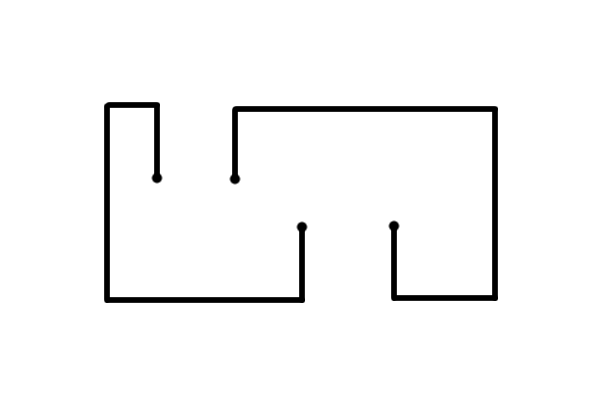
\includegraphics[scale = 0.2]{Bild2.png}};
            \end{tikzpicture}
        \end{center}

        \begin{center}
            \begin{tikzpicture}
                \draw[->] (0,-1) -- (0,0) node {\tiny \textbullet} -- (0,1);
                \draw[->] (-1,0) -- (0,0) -- (1,0);
                \fill[black!60, opacity = 0.6] (-0.05,-0.7) rectangle (0.05,0.7);
                \draw (-0.05,-0.7) rectangle (0.05,0.7);
                \draw (-1.1,0) node[left] {$B=$};
            \end{tikzpicture}
        \end{center}

        \begin{center}
            \begin{tikzpicture}
                \draw (0,0) node[left] {$A \circ B =$} node[right] {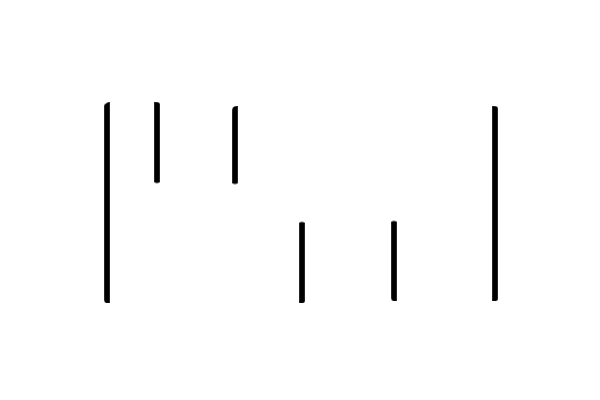
\includegraphics[scale = 0.2]{Bild2open.png}};
            \end{tikzpicture}
        \end{center}

        Bild erzeugt in Matlab durch:\\
        \begin{lstlisting}
I=imread('Bild2.png');
se=strel('line',10,90);
I2=imcomplement(imerode(imcomplement(I),se));
I3=imcomplement(imerode(imcomplement(I2),se));
imshow(I3);
        \end{lstlisting}

\section{Entrauschen: Filter \& Co.}
    \subsection{Rauschen}
        \mim{Rauschen}: Ungewollte Störungen in einem Bild
        \begin{enumerate}[label = \textbullet]
            \item punktweise
            \item zufällig
            \item unabhängig
            \item additiv (bei multiplikativem Rauschen $log$ anwenden)
        \end{enumerate}

        Notation:
        \begin{center}
            \begin{tikzpicture}
                \draw (0,0) rectangle (2,2);
                \draw (1,0) node[below] {\small Sauberes Bild};
                \draw (1,1) node[] {\LARGE $f_0$};
                \draw[->] (2.1,1) -- node[above] {\small $+$ Rauschen} (3.9,1);
                \draw (4,0) rectangle (6,2);
                \draw (5,0) node[below] {\small Gestörtes Bild};
                \draw (5,1) node[] {\LARGE $f$};
                \draw[->] (6.1,1) -- node[above] {\small Entrauschen} (7.9,1);
                \draw (8,0) rectangle (10,2);
                \draw (9,0) node[below] {\small Resultat};
                \draw (9,1) node[] {\LARGE $u$};
            \end{tikzpicture}
        \end{center}

        Wie gut das entrauschte Bild $u$ das saubere Bild $f_0$ beschreibt wird durch Normen gemessen.
	    \begin{align*}
        &\norm{f-f_0}, \text{Rauschen}\\
        &\norm{u-f_0}, \text{\mim{Absoluter Fehler}}\\
        &\frac{\norm{u-f_o}}{\norm{f-f_0}}, \text{\mim{Relativer Fehler} im Vergleich zum Rauschen}\\
        &\frac{\norm{u-f_o}}{\norm{f_0}}, \text{Relativer Fehler im Vergleich zum Signal}
        \end{align*}

        Typischerweise ist die gewählte Norm:
        \[\norm{f} = \norm{f}_2 = \sqrt{\int_{\Omega} \abs{f(x)}^2 dx}\]
        oder im diskreten:
        \[\norm{f}_2=\sqrt{\sum_{x \in \Omega} \abs{f(x)}^2}\]

        Eng verwandt ist die \mim{Signal to noise ratio} (SNR):
        \[log(\underbrace{\frac{\norm{f_0}_2}{\norm{u-f_0}_2}}_{\in \ [1,\infty)}) \in [0,+\infty), \text{ wobei $0$ schlecht und $+\infty$ gut ist.}\]
    \subsection{Glättungsfilter}
        Grundidee: (zur Vereinfachung in 1D)
        \begin{center}
            \begin{tikzpicture}
                \draw (0,0) node[left] {$f_0$:};
                \draw[thick] plot [smooth, tension = 0.7] coordinates {(0,0) (1.75,1.5) (3.5,0.5) (6,2) (9,0) (11,0.5)};
                \draw[->,thick] (-0.3,-0.5) -- node[left] {Rauschen} (-0.3,-2);
                \draw (0,-2.5) node[left] {$f$:};
                \draw[thick, name path = P2,shift = {(0,-2.5)}] plot [smooth, tension = 0.7] coordinates {(0,0) (1.75,1.5) (3.5,0.5) (6,2) (9,0) (11,0.5)};
                \draw[name path = P1, draw = none] (0,-1.1) -- (3,-1.1);
                \draw[name intersections={of = P1 and P2},red,thick]
                (intersection-1) edge[bend right] ++(0.3,0.5) ++(0.3,0.5) edge[bend right] (intersection-2);
                \draw[name path = P3,draw = none] (3,-2.3) -- (5,-1.2);
                \draw[name intersections={of = P3 and P2},red,thick]
                (intersection-1) edge[bend left] ++(0.3,-0.3) ++(0.3,-0.3) edge[bend left] (intersection-2);
                \draw[] (2,-0.9) -- ++(0.5,-0.1) node[right] {\small Störungen} (3.5,-2.1) -- ++(-0.5,0.9);
                \draw (0,-5) node[left] {$f$:};
                \draw[thick, name path = P4,shift = {(0,-5)}] plot [smooth, tension = 0.7] coordinates {(0,0) (1.75,1.5) (3.5,0.5) (6,2) (9,0) (11,0.5)};
                \draw[name path = P5, shift = {(0,-2.5)}, draw = none] (0,-1.1) -- (3,-1.1);
                \draw[name intersections={of = P4 and P5},red,thick]
                (intersection-1) edge[bend right] node[black,pos=0] {\small \textbullet} ++(0.3,0.5) ++(0.3,0.5) edge[bend right] node[black,pos=1] {\small \textbullet}  node[black,pos=0] {\small \textbullet} (intersection-2);
                \draw[name path = P6, shift = {(0,-2.5)}, draw = none] (3,-2.3) -- (5,-1.2);
                \draw[name intersections={of = P4 and P6},red,thick]
                (intersection-1) edge[bend left] node[black,pos=0] {\small \textbullet} ++(0.3,-0.3) ++(0.3,-0.3) edge[bend left] node[black,pos=1] {\small \textbullet}  node[black,pos=0] {\small \textbullet} (intersection-2);
                \draw[decorate,decoration={brace,amplitude=2pt,mirror}] (1.4,-3.7) -- (2.2,-3.7);
                \draw[thick] (1.8,-3.8) -- (1.8,-4.3) node[below] {\small \framebox{Mittelwert}};
                \draw[->,thick,double] (1.6,-5) -- (0.4,-5);
                \draw[->,thick,double] (2,-5) -- (3.2,-5);
                \draw[->,thick] (1.8,-5.1) -- (1.8,-5.7);
                \draw (0,-7.5) node[left] {$u$:};
                \draw[->,thick] (-0.3,-5.5) -- node[left] {Entrauschen} (-0.3,-7);
                \draw[thick, name path = P7,shift = {(0,-7.5)}] plot [smooth, tension = 0.7] coordinates {(0,0) (1.75,1.5) (3.5,0.5) (6,2) (9,0) (11,0.5)};
                \draw[name path = P8, shift = {(0,-5)}, draw = none] (0,-1.2) -- (3,-1.2);
                \draw[name intersections={of = P7 and P8},red,thick]
                plot [smooth,tension=0.7] coordinates {(intersection-1) ($(intersection-1) + (0.5,0.35)$) (intersection-2)};
                \draw[name path = P9, shift = {(0,-5)}, draw = none] (3,-2.25) -- (5,-1.15);
                \draw[name intersections={of = P7 and P9},red,thick]
                plot [smooth,tension=0.7] coordinates {(intersection-1) ($(intersection-1) + (0.45,0.05)$) (intersection-2)};
            \end{tikzpicture}
        \end{center}

        \begin{equation} \label{eq:5.1}
            u(k):=\alpha \cdot f(k-1) + \beta \cdot f(k) + \gamma \cdot f(k+1)
        \end{equation}
        wobei:
        \begin{equation} \label{eq:5.2}
            \alpha + \beta + \gamma = 1
        \end{equation}

        Schematisch bedeutet \eqref{eq:5.1}:

        \begin{center}
            \begin{tikzpicture}
                \draw (0,-0.5) node[left] {\large f:};
                \draw[thick] (0.5,0) grid (6.5,-1);
                \draw (0.5,-0.5) node {\LARGE ...};
                \draw (6.5,-0.5) node {\LARGE ...};
                \draw (1.5,0) node[above] {\dots};
                \draw (2.5,0) node[above] {k-1};
                \draw (3.5,0) node[above] {k};
                \draw (4.5,0) node[above] {k+1};
                \draw (5.5,0) node[above] {\dots};
                \draw (0.5,-2.5) node {\LARGE ...};
                \draw (6.5,-2.5) node {\LARGE ...};

                \draw[->,red] (1.6,-1.1) -- node[left] {\tiny $\alpha$} (2.4,-1.9);
                \draw[->,red] (2.6,-1.1) -- node[left] {\tiny $\alpha$} (3.4,-1.9);
                \draw[->,red] (3.6,-1.1) -- node[left] {\tiny $\alpha$} (4.4,-1.9);
                \draw[->,black!40!green] (2.5,-1.1) -- node[left, pos = 0.3] {\tiny $\beta$} (2.5,-1.9);
                \draw[->,black!40!green] (3.5,-1.1) -- node[left, pos = 0.3] {\tiny $\beta$} (3.5,-1.9);
                \draw[->,black!40!green] (4.5,-1.1) -- node[left, pos = 0.3] {\tiny $\beta$} (4.5,-1.9);
                \draw[->,black!40!blue] (3.4,-1.1) -- node[right, pos = 0.75] {\tiny $\gamma$} (2.6,-1.9);
                \draw[->,black!40!blue] (4.4,-1.1) -- node[right, pos = 0.75] {\tiny $\gamma$} (3.6,-1.9);
                \draw[->,black!40!blue] (5.4,-1.1) -- node[right, pos = 0.75] {\tiny $\gamma$} (4.6,-1.9);

                \draw (0,-2.5) node[left] {\large u:};
                \draw[thick] (0.5,-2) grid (6.5,-3);
            \end{tikzpicture}
        \end{center}

        \begin{center}
            \begin{tikzpicture}
                \draw (-0.6,-0.5) node {\LARGE ...};
                \draw (1.6,-0.5) node {\LARGE ...};
                \draw (-1.6,-2.5) node {\LARGE ...};
                \draw (2.6,-2.5) node {\LARGE ...};
                \draw (0.5,0) node[above] {k};
                \draw[thick] (-0.6,0) grid (1.6,-1);
                \draw[->,red] (0.4,-1.1) -- node[left] {$\alpha$} (-0.5,-1.9);
                \draw[->,black!40!green] (0.5,-1.1) -- node[left] {$\beta$} (0.5,-1.9);
                \draw[->,black!40!blue] (0.6,-1.1) -- node[right] {$\gamma$} (1.5,-1.9);
                \draw[thick] (-1.6,-2) grid (2.6,-3);
            \end{tikzpicture}
        \end{center}

        Durch \eqref{eq:5.1} ist eine Abbildung $f \mapsto u$ gegeben, wir schreiben kurz:
        \[u = m \boxast f, \ \text{dieses wird \mim{Korrelation} genannt.}\]
        mit:
        \begin{equation}\label{eq:5.3}
            \framebox{$\displaystyle (m \boxast f)(k) = \sum_{i \in supp(m)} m(i) f(k+i)$}
        \end{equation}
        und:
        \begin{center}
            \begin{tikzpicture}
                \draw (0,0.5) node[left] {m=};
                \draw[thick] (0.5,0) grid (4.5,1);
                \draw (0.5,0.5) node {\large \dots};
                \draw (1.5,0.5) node {\large $\alpha$};
                \draw (2.5,0.5) node {\large $\beta$};
                \draw (3.5,0.5) node {\large $\gamma$};
                \draw (4.5,0.5) node {\large \dots};
                \draw (0.5,1) node[above] {\large \dots};
                \draw (1.5,1) node[above] {\large -1};
                \draw (2.5,1) node[above] {\large 0};
                \draw (3.5,1) node[above] {\large 1};
                \draw (4.5,1) node[above] {\large \dots};
                \draw (5,0.5) node[right] {genannt \mim{Maske}.};
            \end{tikzpicture}
        \end{center}

        Setzt man nun $j:= k + i$ in \eqref{eq:5.1}, so ist $i=j-k$, d.h.
        \begin{equation}\label{eq:5.4}
            \framebox{$\displaystyle (m \boxast f)(k) = \sum_{i \in supp(m)} m(j-k) f(j)$}
        \end{equation}

        Um die Abbildung auf den Rand anzuwenden wird das Bild gespiegelt, in 1D:
        \begin{center}
            \begin{tikzpicture}
                \draw[step = 0.5] (0,0) grid (2.2,-0.5);
                \draw (2.5,-0.25) node {\large ...};
                \draw[step = 0.5] (2.8,0) grid (5,-0.5);
                \draw[thick] (0,0.1) -- (0,-0.6);
                \draw[thick] (5,0.1) -- (5,-0.6);
                \draw[step = 0.5, dotted] (0,0) grid (-1.2,-0.5);
                \draw[step = 0.5, dotted] (5,0) grid (6.2,-0.5);
                \draw[] (0.25,0.1) edge[bend right = 60, ->] (-0.25,0.1);
                \draw[] (0.75,0.1) edge[bend right = 60, ->] node[above] {\small spiegeln} (-0.75,0.1);
                \draw[] (4.75,0.1) edge[bend left = 60, ->] (5.25,0.1);
                \draw[] (4.25,0.1) edge[bend left = 60, ->] node[above] {\small spiegeln} (5.75,0.1);
                \draw[step = 0.5] (0,-1) grid (2.2,-1.5);
                \draw (2.5,-1.25) node {\large ...};
                \draw[step = 0.5] (2.8,-1) grid (5,-1.5);
                \draw[->] (0.25,-0.55) -- (0.25,-0.95);
                \draw[->] (-0.25,-0.55) -- (0.15,-0.95);
                \draw[->] (0.75,-0.55) -- (0.35,-0.95);
                \draw[->] (4.75,-0.55) -- (4.75,-0.95);
                \draw[->] (4.25,-0.55) -- (4.65,-0.95);
                \draw[->] (5.25,-0.55) -- (4.85,-0.95);
            \end{tikzpicture}
        \end{center}

        in 2D:

        \begin{center}
            \begin{tikzpicture}
                \draw[step =2, thick] (0,0) grid (6,6);
                \draw (3,3) node {\Huge P};
                \draw (1,1) node[rotate = 180] {\Huge P};
                \draw (5,1) node[rotate = 180] {\Huge P};
                \draw (1,5) node[rotate = 180] {\Huge P};
                \draw (5,5) node[rotate = 180] {\Huge P};
                \draw (3,5) node[yscale=-1,xscale=1] {\Huge P};
                \draw (5,3) node[rotate = 180,yscale=-1,xscale=1] {\Huge P};
                \draw (1,3) node[rotate = 180,yscale=-1,xscale=1] {\Huge P};
                \draw (3,1) node[yscale=-1,xscale=1] {\Huge P};
            \end{tikzpicture}
        \end{center}

        Formel \eqref{eq:5.4} erinnert an die Formel der \mim{Faltung}:
        \begin{equation}\label{eq:5.5}
            \framebox{$\displaystyle (g * f)(k) = \sum_{j \in \Z} g(\underbrace{k-j}_{\text{Anders als \eqref{eq:5.4}}}) \cdot f(j)$}
        \end{equation}

        Setzt man also $g(i) := m(-i) =: \tilde m(i)$, was einer Spieglung der Maske entspricht, dann ist
        \[m \boxast f = g * f = \tilde m * f\]

        Eigenschaften der Faltung:
        \begin{enumerate}[label=\framebox{\arabic *}]
            \item $(f * g) * h = f * (g* h)$, Assoziativität
            \item $f*g=g*f$, Kommutativität
            \item $\tilde f * \tilde g = \widetilde{f * g}$, Kompatibilität mit Spiegelung
        \end{enumerate}
        Eigenschaften der Korrelation:
        \begin{enumerate}[label=\framebox{\arabic *'}]
            \item $f \boxast (g \boxast h) = \tilde f * ( \tilde g* h) \overset{\framebox{\small 1}}{=} ( \tilde f * \tilde g) * h \overset{\framebox{\small 3}}{=} (\widetilde{f * g}) * h = (f * g) \boxast h \neq (f \boxast g) \boxast h$, nicht assoziativ!
            \item $f \boxast g = \tilde f * g \overset{\framebox{\small 2}}{=} g * \tilde f = \tilde{\tilde g} * \tilde f \overset{\framebox{\small 3}}{=} \widetilde{(\tilde g * f)} = \widetilde{g \boxast f} \neq g \boxast f$, nicht kommutativ!
            \item $\tilde f \boxast \tilde g = \tilde{\tilde f} * \tilde g \overset{\framebox{\small 3}}{=} \widetilde{(\tilde f * g)} = \widetilde{f \boxast g}$, Kompatibilität mit Spiegelung
        \end{enumerate}

	$\boxast$ und $*$ definiert man auf: $\ell^1(\Z^d):=\{f=(f_i)_{i \in \Z^d} : \underbrace{\sum_{i \in \Z^d}\abs{f_i}}_{:=\norm{f}_1} < \infty\}$

	Man kann zeigen (Übung): $f,g \in \ell^1 \Rightarrow f * g \in \ell^1$ und $\norm{f * g}_1 \leq \norm{f}_1 \C \norm{g}_1$.
    Wobei oft die Gleichheit gilt.

    Alles gilt auch in der Kontinuierlichen Version:
    \[L^1(\R^d) := \{f:\R^d \to \R | \underbrace{\int_{\R^d}\abs{f} dx}_{:=\norm{f}_1} < \infty\}\]
    \[f,g \in L^1(\R^d): (g*f)(x)=\int_{\R^d}g(x-y)f(y) dy, \ y,x \in \R^d\]

    Beispiel für den kontinuierlichen Fall:
    \begin{center}
        \begin{tikzpicture}
            \draw[dotted] (0,1) node[left] {$\frac{1}{2a}$} -- (8,1);
            \draw (0,0) node[left] {$g:$} -- (2.5,0) -- (2.5,1) -- (5.5,1) -- (5.5,0) -- (8,0);
            \draw (2.5,0) node[below] {\small $-a$};
            \draw[dotted] (4,0) node[below] {\small $0$} -- (4,1.5);
            \draw (5.5,0) node[below] {\small $-a$};
        \end{tikzpicture}
    \end{center}
    Hierbei gilt $\displaystyle \int_{\R} g(x) dx = 1$

    \begin{center}
        \begin{tikzpicture}
            \draw[thick, name path = P2] node [left] {$f:$}plot [smooth, tension = 0.45] coordinates {(0,0) (1.2,1.5) (2.1,0.3) (3,2) (4.3,1) (5.3,1.6) (6.6,0.5) (7.5,1) (8,0)};
        \end{tikzpicture}
    \end{center}

    $g \boxast f = $ \mim{gleitendes Mittel}.\\

        \begin{tikzpicture}
            \draw[dotted] (0,1) node[left] {$\frac{1}{2a}$} -- (8,1);
            \draw (0,0) node[left] {$g \boxast g = \tilde g * g = g * g=$} -- (1,0) -- (4,1) -- (7,0) -- (8,0);
            \draw (1,0) node[below] {\small $-2a$};
            \draw[dotted] (4,0) node[below] {\small $0$} -- (4,1.5);
            \draw (7,0) node[below] {\small $-2a$};
        \end{tikzpicture}

    Weitere Eigenschaften der Faltung:\\
    Für alle $f,g \in L^1$ or $\ell ^1$
    \begin{equation*}
        \left.\begin{aligned}
            (g_1 + g_2) * f = (g_1 * f) + (g_2 * g)\\
            (\alpha g) * f = \alpha (g * f)
        \end{aligned}\right\}=\text{Linearität}
    \end{equation*}
    Somit ist:
    \[g \mapsto f * g\]
    ein linearer Operator.

    Formt $\ell^1$ bzw. $L^1$ eine Algebra mit neutralem Element $\delta$?

    $\ell^1$?:
    \begin{center}
        \begin{tikzpicture}
            \draw (0,-0.5) node[left] {\large $\delta$:};
            \draw[thick] (0.5,0) grid (6.5,-1);
            \draw (0.5,-0.5) node {\LARGE ...};
            \draw (6.5,-0.5) node {\LARGE ...};
            \draw (1.5,-0.5) node {\LARGE 0};
            \draw (2.5,-0.5) node {\LARGE 0};
            \draw (3.5,-0.5) node {\LARGE 1};
            \draw (4.5,-0.5) node {\LARGE 0};
            \draw (5.5,-0.5) node {\LARGE 0};
            \draw[->] (3.5,-1.4) node[below] {Pos $0$} -- (3.5,-1.1);
        \end{tikzpicture}
    \end{center}
    Ja!

    $L^1$?:
    Für ein solches Element muss gelten:\\
    $\forall f \in L^1 : d * f = f$\\
    $\forall x \in \R :\displaystyle \int_{\R^d} \underbrace{\delta(x-y)}_{=0 \forall x \neq y} f(y) dy = f(x)$

    Diese Funktion wird \mim{Dirac-Impuls} genannt ist aber kein Element von $L^1$.

    \pa{Nun zu Masken in 2D:}

    \begin{equation*}
        u = m \boxast f \text{ mit } m= \raisebox{-0.665cm}{\begin{tikzpicture}
            \draw[step = 0.5] (0,0) grid (0.5,1.5);
            \draw[step = 0.5] (-0.5,1) grid (1,0.5);
            \draw (0.25,1.25) node {$\alpha$};
            \draw (0.25,0.75) node {$\gamma$};
            \draw (0.25,0.25) node {$\epsilon$};
            \draw (-0.25,0.75) node {$\beta$};
            \draw (0.75,0.75) node {$\delta$};
        \end{tikzpicture}}
    \end{equation*}
    wobei $\alpha + \beta +\gamma +\delta + \epsilon = 1$\\
    Kurzschreibweise: $u_{ij}:=u(x)$ wobei $x = \begin{pmatrix}i\\j\end{pmatrix} \in \Z^2$, analog für $f_{ij}$.

    \[\Rightarrow u_{ij} = \alpha f_{i-1,j} + \beta f_{i,j-i} + \gamma f_{ij} + \delta f_{i,j+1} + \epsilon f_{i+1,j}\]

    \begin{equation*}
        u = m \boxast f = \tilde m * f \text{ mit } \tilde m = \raisebox{-0.665cm}{\begin{tikzpicture}
            \draw[step = 0.5] (0,0) grid (0.5,1.5);
            \draw[step = 0.5] (-0.5,1) grid (1,0.5);
            \draw (0.25,1.25) node {$\epsilon$};
            \draw (0.25,0.75) node {$\gamma$};
            \draw (0.25,0.25) node {$\alpha$};
            \draw (-0.25,0.75) node {$\delta$};
            \draw (0.75,0.75) node {$\beta$};
        \end{tikzpicture}}
    \end{equation*}

    \pa{Symmetrischer Fall:}

    \begin{equation*}
    \tilde m = \raisebox{-0.665cm}{\begin{tikzpicture}
            \draw[step = 0.5] (0,0) grid (0.5,1.5);
            \draw[step = 0.5] (-0.5,1) grid (1,0.5);
            \draw (0.25,1.25) node {$\alpha$};
            \draw (0.25,0.75) node {$\gamma$};
            \draw (0.25,0.25) node {$\alpha$};
            \draw (-0.25,0.75) node {$\alpha$};
            \draw (0.75,0.75) node {$\alpha$};
        \end{tikzpicture}} \text{ mit } \gamma = 1 - 4 \alpha
    \end{equation*}

    \begin{equation}
        u_{ij} = (1 - 4 \alpha)f_{ij} + \alpha(f_{i-1,j} + f_{i,j-1} + f_{i,j+1} + f_{i+1,j})
    \end{equation}

    \begin{equation*}
            \text{Erinnerung: } \raisebox{-1.2cm}{\begin{tikzpicture}[scale=0.9]
                \draw (0,0) rectangle (2,2);
                \draw (1,0) node[below] {\small Sauberes Bild};
                \draw (1,1) node[] {\LARGE $f_0$};
                \draw[->] (2.1,1) -- node[above] {\small $+$ Rauschen} (3.9,1);
                \draw (4,0) rectangle (6,2);
                \draw (5,0) node[below] {\small Gestörtes Bild};
                \draw (5,1) node[] {\LARGE $f$};
                \draw[->] (6.1,1) -- node[above] {\small Entrauschen} (7.9,1);
                \draw (8,0) rectangle (10,2);
                \draw (9,0) node[below] {\small Resultat};
                \draw (9,1) node[] {\LARGE $u$};
            \end{tikzpicture}}
    \end{equation*}

    Annahme: $f_{ij} = f_{ij} +r_{ij}$ mit $r_{ij} \sim N(0,\sigma^2)$ iid.

    z.z.: $Var(u_{ij}) \leq Var(f_{ij})$\\

    \begin{equation*}
        Var(f_{ij}) = E(\underbrace{f_{ij} - \overbrace{E f_{ij}}^{f^0_{ij}}}_{r_{ij}})^2 = \sigma^2
    \end{equation*}

    \begin{align*}
        Var(u_{ij}) &= E(u_{ij} - E u_{ij})^2 = E((1 - 4 \alpha) (\underbrace{f_{ij} - f^0_{ij}}_{r_{ij}}) + \alpha(\underbrace{(f_{i-1,j} - f^0_{i-1,j})}_{r_{i-1,j}} + ... + \underbrace{(f_{i+1,j} - f^0_{i+1,j})}_{r_{i+1,j}}))^2\\
        &= E((1 - 4 \alpha)^2 r_{ij}^2 + \alpha^2(r_{i-1,j}^2 + r_{i,j-1}^2 +r_{i,j+1}^2 + r_{i+1,j}^2) + 2 (1 - 4 \alpha) \alpha r_{ij} r_{i-1,j}...)\\%TODO fix this mess
        &= (1 - 4 \alpha)^2 \underbrace{E r_{i,j}^2}_{\sigma^2} + \alpha^2(E r_{i-1,j}^2 + ... + E r_{i+1,j}^2) + 2 (1 - 4 \alpha) \alpha \underbrace{E(r_{ij}r_{i-1,j})}_{\underbrace{E r_{ij} E r_{i-1,j}}_{0}} + \underbrace{...}_{0})\\
        &=(1 - 4 \alpha)^2 \sigma^2 + \alpha^2 4 \sigma^2 = (1 - 8 \alpha + 16 \alpha ^2 + 4 \alpha^2) \sigma^2
    \end{align*}

    Da $0 \leq \alpha$ und $ 0 \leq 1 - 4 \alpha \Rightarrow 0 \leq \alpha \leq \frac{1}{4}$:

    \begin{equation*}
        (1 - 8 \alpha + 16 \alpha ^2 + 4 \alpha^2) \sigma^2 = \underbrace{1 + \underbrace{20 \alpha}_{\geq 0} (\underbrace{\alpha - \frac{2}{5}}_{< 0})}_{\leq 1}
    \end{equation*}

    $\Rightarrow Var(u_{ij}) \leq Var(f_{ij})$ für $\alpha \in [0,\frac{1}{4}]$\\

    Dabei gilt: $Var(u_{ij}) \overset{\alpha}{\to} d \text{min} \iff 1 - 8 \alpha + 20 \alpha^2 \overset{\alpha}{\to} \text{min} \iff -8 + 40 \alpha = 0 \iff \alpha = \frac{1}{5}$

    \begin{equation*}
        \Rightarrow \text{bester Filter} : \ \raisebox{-0.9cm}{\begin{tikzpicture}[scale = 1.3]
                \draw[step = 0.5] (0,0) grid (0.5,1.5);
                \draw[step = 0.5] (-0.5,1) grid (1,0.5);
                \draw (0.25,1.25) node {$\frac{1}{5}$};
                \draw (0.25,0.75) node {$\frac{1}{5}$};
                \draw (0.25,0.25) node {$\frac{1}{5}$};
                \draw (-0.25,0.75) node {$\frac{1}{5}$};
                \draw (0.75,0.75) node {$\frac{1}{5}$};
            \end{tikzpicture}}
        \end{equation*}

    \subsection{Frequenzraum-filter}
        Ansatz: Rauschen = hochfrequente Anteile des Signals.\\
        Diese können mittels der \mim{Fouriertransformation} $\mathcal F$ gezielt entfernt werden.

        \begin{equation*}
            \begin{tikzpicture}[scale = 0.9]
                \draw (0,0) rectangle (2,2);
                \draw (1,0) node[below] {\small Sauberes Bild};
                \draw (1,1) node[] {\LARGE $f_0$};
                \draw[->] (2.1,1) -- node[above] {$+r$} (2.9,1);
                \draw (3,0) rectangle (5,2);
                \draw (4,0) node[below] {\small Gestörtes Bild};
                \draw (4,1) node[] {\LARGE $f$};
                \draw[->] (5.1,1) -- node[above] {$\mathcal F$} (5.9,1);
                \draw (6,-0.5) rectangle (9,2.5);
                \draw (6,1) -- (9,1);
                \draw[thick, name path = P2]plot [smooth, tension = 0.8] coordinates {(6,1) (6.1,1.3) (6.4,1.1) (6.6,1.6) (7,1.1) (7.3,2.0) (7.5,1.1) (7.7,1.2) (7.8,1.9) (8.1,1.5) (8.5,1.9) (9,1)};
                \draw[->] (9.1,1) -- node[above] {\small Abschneiden} (10.9,1);
                \draw[->] (14.1,1) -- node[above] {$\mathcal F^{-1}$} (14.9,1);
                \draw[decorate,decoration={brace,amplitude=2pt,mirror}] (6,0.6) -- node[below] {\scriptsize \begin{tabular}{c} niedrige \\ Frequenzen \end{tabular}} (7.5,0.6);
                \draw[decorate,decoration={brace,amplitude=2pt,mirror}] (7.5,0.6) -- node[below] {\scriptsize \begin{tabular}{c} hohe \\ Frequenzen \end{tabular}} (9,0.6);
                \draw[thick, name path = P2,shift = {(5,0)}]plot [smooth, tension = 0.8] coordinates {(6,1) (6.1,1.3) (6.4,1.1) (6.6,1.6) (7,1.1) (7.3,2.0) (7.5,1.1) (7.7,1.2) (7.8,1.9) (8.1,1.5) (8.5,1.9) (9,1)};
                \draw[color = white,fill] (12.7,1) rectangle (14,2.5);
                \draw (11,1) -- (14,1);
                \draw (11,-0.5) rectangle (14,2.5);
                \draw (15,0) rectangle (17,2);
                \draw[thick] (7.7,0.8) -- (7.7,2.3);
                \draw[thick] (12.7,0.8) -- (12.7,2.3);
                \draw (16,1) node[] {\LARGE $u$};
                \draw[decorate,decoration={brace,amplitude=2pt,mirror}] (5.5,-1) -- node[below] {im Frequenzbereich} (14.5,-1);
                \draw[decorate,decoration={brace,amplitude=2pt,mirror}] (3,-1.5) -- node[below] {\mim{Frequenzraumfilter} (Tiefpass)} (17,-1.5);
            \end{tikzpicture}
    \end{equation*}

    Ein wichtiges Instrument ist hierbei die Fouriertransformation:
    \[\mathcal F : f \mapsto \hat f\]
    \begin{equation}
        \boxed{\hat f(z) = \frac{1}{(2 \pi)^\frac{d}{2}} \int_{\R^d} f(x) e^{-i \skprod{z}{x}} dx}
    \end{equation}

    Wobei  $z \in \R^d, f \in L^1(\R^d)$.

    Falls auch $\hat f \in L^1(\R^d)$ ist ,dann lässt sich $f$ wie folgt mittels der inversen Fouriertransformation aus $\hat f$ rekonstruieren:

    \[\mathcal F^{-1} : \hat f \mapsto f\]
    \begin{equation}
        \boxed{\hat f(z) = \frac{1}{(2 \pi)^\frac{d}{2}} \int_{\R^d} f(x) e^{i \skprod{z}{x}} dx}
    \end{equation}
    Wobei $x \in \R^d$.\\

    Man hat also $\mathcal F^{-1} \mathcal F f$, d.h.

    \[f(x) = \frac{1}{(2 \pi)^\frac{d}{2}} \int_{\R^d} \left(\frac{1}{(2 \pi)^\frac{d}{2}} \int_{\R^d} f(y) e^{-i \skprod{z}{y}} dy\right) e^{i \skprod{z}{x}} dz\]

    Sei nun $e_z(x) := e^{i \skprod{z}{x}}, \ x \in \R^d$ mit Parameter
$z = \srmatrix{z_1 \\ \vdots \\ z_d}$.\\
    Also $e_z(x) = e^{i\skprod{\srmatrix{z_1\\z_2}}{\srmatrix{x_1\\x_2}}} = e^{i (z_1 x_1 +z_2 x_2)}$\\
    Beispiele in $2D$:\\
    (Hier stellen die Linien, Punkte mit konstantem wert dar)

    \begin{minipage}[t]{0.49\linewidth}
        \begin{center}
            $z = \srmatrix{1 \\ 0}, \  e_z(x)=e^{ix_1}$:\\
            \begin{tikzpicture}
                \draw[->] (-1.1,0) -- (4,0) node[right] {$x_1$};
                \draw[->] (0,-1.1) -- (0,4) node[above] {$x_2$};
                \foreach \i in {-0.7, 0.3, 1.3, 2.3, 3.3}{
                    \draw[thick] (\i,-0.6) -- (\i,4.1);
                }
            \end{tikzpicture}

            $z = \srmatrix{0 \\ 1}, \  e_z(x)=e^{ix_2}$:\\
            \begin{tikzpicture}
                \draw[->] (-1.1,0) -- (4,0) node[right] {$x_1$};
                \draw[->] (0,-1.1) -- (0,4) node[above] {$x_2$};
                \foreach \i in {-0.7, 0.3, 1.3, 2.3, 3.3}{
                    \draw[thick] (-0.6,\i) -- (4.1,\i);
                }
            \end{tikzpicture}

            $z = \srmatrix{1 \\ 1}, \  e_z(x)=e^{i(x_1 + x_2}$:\\
            \begin{tikzpicture}
                \draw[->] (-1.1,0) -- (4,0) node[right] {$x_1$};
                \draw[->] (0,-1.1) -- (0,4) node[above] {$x_2$};
                \foreach \i in {-2.6, -1.6, -0.6, 0.4, 1.4}{
                    \draw[thick, rotate = -45,shift={(0,\i)}] (-2,2) -- (2,2);
                }
            \end{tikzpicture}
        \end{center}
    \end{minipage}
    \hfill
    \begin{minipage}[t]{0.49\linewidth}
        $z = \srmatrix{2 \\ 0}, \ e_z(x)=e^{i2x_1}$:\\
        \begin{tikzpicture}
            \draw[->] (-1.1,0) -- (4,0) node[right] {$x_1$};
            \draw[->] (0,-1.1) -- (0,4) node[above] {$x_2$};
            \foreach \i in {-0.7, -0.2, 0.3, 0.8, 1.3, 1.8, 2.3, 2.8, 3.3}{
                \draw[thick] (\i,-0.6) -- (\i,4.1);
            }
        \end{tikzpicture}

        $z = \srmatrix{0 \\ 2}, \  e_z(x)=e^{i2x_2}$:\\
        \begin{tikzpicture}
            \draw[->] (-1.1,0) -- (4,0) node[right] {$x_1$};
            \draw[->] (0,-1.1) -- (0,4) node[above] {$x_2$};
            \foreach \i in {-0.7, -0.2, 0.3, 0.8, 1.3, 1.8, 2.3, 2.8, 3.3}{
                \draw[thick] (-0.6,\i) -- (4.1,\i);
            }
        \end{tikzpicture}

        $z = \srmatrix{-2 \\ 1}, \  e_z(x)=e^{i(-2x_1 + x_2)}$:\\
        \begin{tikzpicture}
            \draw[->] (-1.1,0) -- (4,0) node[right] {$x_1$};
            \draw[->] (0,-1.1) -- (0,4) node[above] {$x_2$};
            \foreach \i in {-2.8, -1.8, -0.8, 0.2, 1.2}{
                \draw[thick, rotate = 112.5,shift={(0.85*\i,0.85*\i)}] (-1,1) -- (3,-3);
            }
        \end{tikzpicture}
    \end{minipage}

    $\displaystyle f \in L^2(\R^d) = \{f:\R^d \to \R | \int_{\R^d} \abs{f}^2 dx < \infty\}$ ist
    \begin{enumerate}[label = -]
        \item ein normierter Raum mit $+$, $\alpha \cdot$ und $\displaystyle \norm{\cdot}_2 := \sqrt{\int_{\R^d} \abs{f(x)}^2 dx}$
        \item ein Skalarproduktraum mit $\displaystyle \skprod{f}{g} := \int_{\R^d} f \bar g dx$, wobei $\norm{f}_2^2=\skprod{f}{f}$
        \item ein vollständiger Raum, also \mim{Banachraum}
    \end{enumerate}
    Ein vollständiger normierter Banachraum mit Skalarprodukt heißt \mim{Hilbertraum}.

    $\mathcal F$ kann auch als Abbildung auf $L^2(\R^d)$ betrachtet werden. Dann gilt:\\
    \[\hat f = \mathcal F f \in L^2(\R^d)\]
    und
    \begin{equation}
        \norm{\hat f}_2 = \norm{f}_2
    \end{equation}
    und sogar
    \begin{equation}
        \skprod{\hat f}{\hat g}_2 = \skprod{f}{g}_2
    \end{equation}
    für alle $f,g \in L^2(\R^d)$.

    Weitere Eigenschaften der Fouriertransformation:

    \begin{enumerate}[label = \roman *)]
        \item $f \in L^1(\R^d) \Rightarrow \hat f$ stetig und $\underset{\abs{z} \to \infty}{lim} \hat f(z) = 0$
        \item $\mathcal F: L^1(\R^d) \to C(\R^d)$ ist eine lineare Abbildung
        \item $\mathcal F: L^1(\R^d) \to C(\R^d)$ ist eine beschränkte/stetige Abbildung
        \item Verschiebung $\overset{\mathcal F}{\to}$ Modulation, d.h.
        \begin{equation*}
            g(x) = f(x+a) \Rightarrow \hat g(z) = e^{i \skprod{a}{z}} \hat f(z)
        \end{equation*}
        \item Modulation $\overset{\mathcal F}{\to}$ Verschiebung, d.h.
        \begin{equation*}
            g(x) = e^{i \skprod{x}{a}} f(x) \Rightarrow \hat g(z)= \hat f(z-a)
        \end{equation*}
        \item Skalierung $\overset{\mathcal F}{\to}$ inverse Skalierung, d.h.
        \begin{equation*}
            g(x)=f(cx) \Rightarrow \hat g(z) = \frac{1}{\abs c} \hat f(\frac{z}{\abs c})
        \end{equation*}
        \item Konjugation: $g(x) = \overline{f(x)} \Rightarrow \hat g(z) = \overline{\hat f (-z)}$\\
        Folglich: $f$ reelwertig $\Rightarrow \hat f(z) = \overline{\hat f(-z)}$
        \item
        \begin{align*}
            \text{Grundmode:} \ & \displaystyle \hat f(0) = \frac{1}{(2 \pi )^\frac{d}{2}} \int_{\R^d} f(x) dx\\
            \text{Analog:} \ & \displaystyle f(0) = \frac{1}{(2 \pi )^\frac{d}{2}} \int_{\R^d} \hat f(x) dx
        \end{align*}
        \item Differentiation $\overset{\mathcal F}{\to}$ Multiplikation mit Potenzen von z, d.h.
        \begin{equation*}
            g(x) = \frac{\partial^{\alpha_1 + \cdots + \alpha_d}}{\partial x_1^{\alpha_1} \cdots \partial x_d^{\alpha_d}} f(x) \Rightarrow \hat g(z) = i^{\alpha_1 + \cdots + \alpha_d} z_1^{\alpha_1} \cdots z_d^{\alpha_d} \hat f(z)
        \end{equation*}
        \item Umkehrung des letzten Punktes:
        \begin{equation*}
            g(x) = x_1^{\alpha_1} \cdots x_d^{\alpha_d} f(x) \Rightarrow \hat g(z) = i^{\alpha_1 + \cdots + \alpha_d}  \frac{\partial^{\alpha_1 + \cdots + \alpha_d}}{\partial x_1^{\alpha_1}} \hat f(z)
        \end{equation*}
        \item
        \begin{align*}
            \text{Faltungssatz:} \  & \mathcal F(f*g) = (2 \pi)^{\frac{d}{2}} \mathcal F(f) \cdot \mathcal F(g), \ \widehat{f*g}=(2 \pi)^{\frac{d}{2}} \hat f \cdot \hat g\\
            \text{Analog:} \ & \mathcal F (f \cdot g) = \frac{1}{(2 \pi)^{\frac{d}{2}}} \mathcal F(f) * \mathcal F(g), \ \widehat{f \cdot g} = \frac{1}{(2\pi)^{\frac{d}{2}}} \hat f * \hat g
        \end{align*}
        d.h.: Faltung $\overset{\mathcal F}{\to}$ Multiplikation und umgekehrt
    \end{enumerate}

    \Large{\textbf{Zur Erinnerung:}}
    \normalsize
    \begin{center}
        \begin{tikzpicture}[scale = 0.9]
            \draw (0,0) rectangle (3,3);
            \draw (1.5,1.5) node[] {\LARGE $f_0$};
            \draw[->] (3.1,1.5) -- node[above] {$\mathcal F$} (3.9,1.5);
            \draw (4,0) rectangle (7,3);
            \draw (5.5,1.5) node[] {\LARGE $\hat f$};
            \draw[->] (7.1,1.5) -- node[above] {\footnotesize \begin{tabular}{c}
                Hohe Frequenzen\\abschneiden
            \end{tabular}} (9.4,1.5);
            \draw (9.5,0) rectangle (12.5,3);
            \draw (11,1.5) node[] {\LARGE $\hat u$};
            \draw[->] (12.6,1.5) -- node[above] {$\mathcal F^{-1}$} (13.4,1.5);
            \draw (13.5,0) rectangle (16.5,3);
            \draw (15,1.5) node[] {\LARGE $u$};

            \draw[thin] (4,-2) -- node[below] {\small 0} (7,-2);
            \draw[thick, name path = P2,shift = {(-2,-3)}]plot [smooth, tension = 0.8]coordinates {(6,1) (6.1,1.3) (6.4,1.1) (6.6,1.6) (7,1.1) (7.3,2.0) (7.5,1.1) (7.7,1.2) (7.8,1.9) (8.1,1.5) (8.5,1.9) (9,1)};
            \draw[decorate,decoration={brace,amplitude=2pt,mirror}] (4.8,-2.5) -- node[below] {\small tiefe Frequenzen} (6.2,-2.5);

            \draw[thick, name path = P2,shift = {(3.5,-3)}]plot [smooth, tension = 0.8]coordinates {(6,1) (6.1,1.3) (6.4,1.1) (6.6,1.6) (7,1.1) (7.3,2.0) (7.5,1.1) (7.7,1.2) (7.8,1.9) (8.1,1.5) (8.5,1.9) (9,1)};
            \draw[fill, color = white] (9.5,-2) rectangle (10.3,-0.5);
            \draw[fill, color = white] (12.5,-2) rectangle (11.7,-0.5);
            \draw[] (11.7,-0.7) -- (11.7,-2.1) node[below] {\small $r$};
            \draw[] (10.3,-0.7) -- (10.3,-2.1) node[below] {\small $-r$};
            \draw[thin] (9.5,-2) -- (12.5,-2);
            \draw (11,-2.1) node[below] {\small 0};

            \draw[->] (5.5,-3) -- (5.5,-3.5) -- (11,-3.5) -- (11,-2.7);

            \draw[shift = {(0.25,-0.3)}] (6.25,-3.8) node[] {\small \textbullet} (6.5,-4) -- (7,-4) node[below] {\small $-r$} -- (7,-3.6) -- (9,-3.6) -- (9,-4) node[below] {\small $r$} -- (9.5,-4) (8,-4) node[below] {\small 0};

        \end{tikzpicture}
    \end{center}

    \begin{center}
        \begin{tikzpicture}
            \draw[dotted] (-0.3,0) rectangle (-6,-7);
            \draw (-2.5,0) node[above] {\mim{Zeitbereich}};
            \draw[dotted] (0.3,0) rectangle (6,-7);
            \draw (2.5,0) node[above] {\mim{Frequenzbereich}};

            \draw (-3,-1) node[] {$f$};
            \draw (-2.8,-1) edge[bend right=-15,->] node[above, pos = 0.5] {$\mathcal F$} node[below, pos = 0.5] {\small $n \C log(n)$} (2.8,-1);
            \draw (3,-1) node[] {$\hat f$};
            \draw[] (3,-1.5) edge[bend right=-15,->] node[right, pos = 0.5] {\small Mult. mit:} node[left, pos = 0.5] {\small $n$} (3,-5.5);
            \draw (4.05,-4) node[left] {\footnotesize $\hat g:=$};
            \draw (4,-4.1) -- (4.3,-4.1) -- (4.3,-3.8) -- (5,-3.8) -- (5,-4.1) -- (5.3,-4.1) (4.65,-4.1) node[] {\tiny $0$};
            \draw[dotted] (4,-3.8) -- (5.3,-3.8) node[xshift=10] {\footnotesize $\frac{1}{(2 \pi)^\frac{d}{2}}$};
            \draw (3,-6) node[] {$\hat u$} (3,-6.25) node[right] {\small \begin{tabular}{c}
                $= \hat f \cdot \hat g \cdot (2 \pi)^{\frac{d}{2}}$\\
                $= \widehat{f*g}$
            \end{tabular}};
            \draw[] (2.5,-6) edge[bend right=-15,->] node[above, pos = 0.5] {\small $n \cdot log(n)$} node[below, pos = 0.5] {$\mathcal F^{-1}$} (-2.5,-6);
            \draw (-3,-6) node[] {$u$};
            \draw (-3,-6) node[left] {\small $f*g=$};
            \draw (-3,-1.5) edge[bend left=-15,->] node[right,pos = 0.5] {\small $n^2$} node[left, pos = 0.5] {\small Faltung, $*g$} (-3,-5.5);
            \draw [thick, name path = P2,->]plot [smooth, tension = 0.9]coordinates {(-2.5,-1.5) (1.5,-1.5) (1.5,-5) (-2.5,-5.5)};
            \draw (2,-3.5) node[left] {\small $n \cdot log(n)$};
        \end{tikzpicture}
    \end{center}

    Wie sieht $g$ aus?
    \[g = \mathcal F^{-1} \left(\frac{1}{( 2 \pi)^{\frac{d}{2}}} \chi_{[-r,r]}\right)\]

    \small
    \[\left(
    \chi_M(z) =
    \begin{cases}
         0, & z \not \in M\\
         1, & z \in M
    \end{cases}\right)\]

    \normalsize
    \begin{align*}
        g(x) = & \frac{1}{( 2 \pi)^{\frac{d}{2}}}(\mathcal F^{-1} \chi_{[-r,r]^d})(x)\\
        = & \frac{1}{( 2 \pi)^{\frac{d}{2}}} \frac{1}{( 2 \pi)^{\frac{d}{2}}} \int_{\R^d} \chi_{[-r,r]^d}(z) e^{i \skprod{z}{x}} dz\\
        (d=1) \to = & \frac{1}{2 \pi} \int_{-\infty}^{\infty} \chi_{[-r,r]}(z) e^{izx} dz\\
        = & \frac{1}{2 \pi} \int_{r}^{-r} e^{izx} dz\\
        = & \frac{1}{2 \pi}  \frac{e^{izx}}{ix} \Big|_{z=-r}^{r}\\
        = & \frac{1}{2 \pi i x}\left( e^{irx} - e^{-irx} \right)\\
        = & \frac{1}{\pi x} sin(rx)\\
        = & sinc\left(\frac{rx}{\pi}\right) \cdot \frac{r}{\pi}
    \end{align*}

    \[\text{Wobei:\ } sinc(\varphi)=
    \begin{cases}
        \frac{sin(\pi \varphi)}{\pi \varphi} &, \varphi \neq 0\\
        1 &, \varphi = 0
    \end{cases}\]

    $g$ hat auch Masse $1$, denn mit den Eigenschaften der Fouriertransformation folgt:

    \[\frac{1}{( 2 \pi)^{\frac{d}{2}}} = \hat g(0) = (\mathcal F g)(0) = \frac{1}{( 2 \pi)^{\frac{d}{2}}} \int_{R^d} g(x) \underbrace{e^{\underbrace{-\skprod{x}{0}}_0}}_1 dx = \frac{1}{( 2 \pi)^{\frac{d}{2}}} \int_{R^d} g(x) dx\]

    \[\Rightarrow \int_{\R^d} g(x) dx = 1\]

    Für $d=2$ gilt:

    \begin{align*}
        g(x) = & \frac{1}{(2 \pi)^{1}}(\mathcal F^{-1} \chi_{[-r,r]^2})(x)\\
        = & \ \cdots \ (\text{Analog zu oben})\\
        = & \frac{1}{(2 \pi)^{2}} \int_{-\infty}^\infty  \int_{-\infty}^\infty \chi_{[-r,r]^2}\left( \srmatrix{x_1\\x_2} \right) e^{i (z_1 x_1 + z_2 x_2)} dz_1 dz_2\\
        = & \frac{1}{(2 \pi)^{2}} \int_{-r}^r \left( \int_{-r}^r e^{i z_1 x_1} e^{iz_2 x_2} dz_1 \right)dz_2\\
        = & \underbrace{ \left(\frac{1}{2 \pi} \int_{-r}^r e^{i z_1 x_1} dz_1\right) }_{\frac{1}{\pi x_1} sin(\pi x_1)} \underbrace{ \left( \frac{1}{2 \pi} \int_{-r}^r e^{iz_2 x_2} dz_2 \right)}_{\frac{1}{\pi x_2} sin(\pi x_2)}\\
    \end{align*}

    Es ist zu bemerken, dass $g$ eine Art Tensor Struktur besitzt, was in etwa bedeutet das sich die Funktion in beliebigen Dimensionen als Produkt der Funktion in einer Dimensionen darstellen lässt.

    \mim{Gauß-Kern}:
    \begin{align*}
        G(x) =& \frac{1}{(2 \pi)^{\frac{d}{2}}} e^{\frac{-\abs{x}^2}{2}} \Rightarrow G\left( \srmatrix{x_1\\\vdots\\x_d} \right) = \frac{1}{(2 \pi)^{\frac{d}{2}}} e^{\frac{-x_1^2-x_2^2 + \cdots + x_d^2}{2}}\\
        =& \left( \frac{1}{(2 \pi)^\frac{1}{2}} e^{\frac{-x_1^2}{2}}\right) \cdot \ \cdots \ \cdot \left( \frac{1}{(2 \pi)^\frac{1}{2}} e^{\frac{-x_d^2}{2}}\right) = G(x_1) \cdot \ \cdots \ \cdot G(x_d)
    \end{align*}

    \subsection{Filterbreite und Glättung}

    \begin{center}
        \begin{tikzpicture}
            \foreach \i in {0,...,4}
                \foreach \j in {0,...,4}
                    \draw (0.5*\i + 0.25,0.5*\j + 0.25) node[] {\small 1};
            \draw[step = 0.5] (0,0) grid (2.5,2.5);
            \draw (0,1.25) node[left] {klar ist: $\frac{1}{25}$};
            \draw (3,1.25) node[right] {'glättet mehr als': $\frac{1}{9}$};
            \draw[step = 0.5, shift = {(6.5,0.5)}] (0,0) grid (1.5,1.5);
            \foreach \i in {0,...,2}
                \foreach \j in {0,...,2}
                    \draw (0.5*\i + 6.75,0.5*\j + 0.75) node[] {\small 1};
        \end{tikzpicture}
    \end{center}

    Im Kontinuierlichen: Sei $m \in L^1(\R^d)$ und $s > 0$.
    Setze
        $$ m_s(x) := \frac{1}{s^d} m (\frac{x}{s}), \quad x\in \R^d$$

    Bsp (in $d =1 $):
    \begin{center}
        \begin{tikzpicture}
            \draw[->] (-2.2,0) -- (2.2,0) node[right] {\small x};
            \draw[->] (0,-0.1) -- (0,2.2) node[above] {\small y};
            \draw (-2,0.1) -- (-2,-0.1) node[below] {\small $-1$};
            \draw (2,0.1) -- (2,-0.1) node[below] {\small $-1$};
            \draw (0.1,2) -- (-0.1,2) node[left] {\small $1$};
            \draw[thick] (-2,0) -- (0,2) -- (2,0);
            \draw (1.2,1.2) node[rotate = -45] {\small $y=m(x)$};
            \draw[->] (3.8,0) -- (12.2,0) node[right] {\small x};
            \draw[->] (8,-0.1) -- (8,1.2) node[above] {\small y};
            \draw (4,0.1) -- (4,-0.1) node[below] {\small $-1$};
            \draw (2,0.1) -- (2,-0.1) node[below] {\small $-1$};
            \draw (8.1,1) -- (7.9,1) node[left, xshift = -9, yshift = 4] {\small $\frac{1}{2}$};
            \draw[thick] (4,0) -- (8,1) --(12,0);
            \draw (10,0.8) node[rotate = -12.5] {\small $y=m(x)$};
            \draw[->,double] (2,1.5) -- node[above] {\small $s=2$} (4,1.5);
        \end{tikzpicture}
    \end{center}

    Bsp: Gauß-Kern $G(x) = \frac{1}{(2 \pi)^{\frac{d}{2}}} e^{\frac{-\abs{x}^2}{2}}$\\
    Skalierung mit Faktor $s > 0$
    $$ \Rightarrow G_s(x) = \frac{1}{s^d} G\left( \frac {x} {s} \right) = \frac{1}{s^d} \frac{1}{(2 \pi)^{\frac{d}{2}}} e^{\frac{-\abs{x}}{2}} = \frac{1}{(2 \pi s^2)^{\frac{d}{2}}} e^{\frac{-\abs{x}^2}{2s^2}}$$

    Skalierung $s \hat = $ Standardabweichung $\sigma$:

    \begin{center}
        \begin{tikzpicture}
            \draw[scale=1,domain=-2.5:2.5,smooth,variable=\x]  plot ({\x},{(e^((-(\x)^2)/2)});
            \draw[scale=1,domain=-2.5:2.5,smooth,variable=\x,shift={(6,0)}]  plot ({\x},{(1/(2*pi)^(1/2))*e^((-(\x)^2)/2)});
            \draw[->,double] (2.5,0.5) -- (3.5,0.5);
        \end{tikzpicture}
    \end{center}

    \subsection{Differenzenfilter}

    Bisher: Glättung $\widehat =$ Mittelwert bilden $\widehat =$ Summe/Integrale\\
    Jetzt: Schärfen $\widehat =$ Differenzen/Kontraste hervorheben $\widehat =$ Differenzen/Ableitungen\\

    \mtitle{Diskretisierung von Ableitungen durch Differenzenquotienten}
    \ \\
    \begin{minipage}[c]{0.25\linewidth}
        \begin{center}
            \begin{tikzpicture}

                \draw[scale=1,domain=-0.75:1.5,smooth,variable=\x]  plot ({\x},{(\x * \x)});
                \draw[] (-1,-0.3) -- (2,-0.3);
                \draw[dotted] (-0.5,-0.3) node[] {\small \textbullet} node[below] {\small $x_{k-1}$} -- (-0.5,0.25) node[] {\small \textbullet};
                \draw[dotted] (0.25,-0.3) node[] {\small \textbullet} node[below] {\small $x_{k}$} -- (0.25,0.0125) node[] {\small \textbullet};
                \draw[dotted] (1,-0.3) node[] {\small \textbullet} node[below] {\small $x_{k+1}$} -- (1,1) node[] {\small \textbullet};
                \draw[decorate,decoration={brace,amplitude=2pt,mirror}] (-0.5,-0.7) -- node[below] {\small $h$} (0.25,-0.7);
                \draw[dotted] (1,-0.3) node[] {\small \textbullet} node[below] {\small $x_{k+1}$} -- (1,1) node[] {\small \textbullet};
                \draw[decorate,decoration={brace,amplitude=2pt,mirror}] (0.25,-0.7) -- node[below] {\small $h$} (1,-0.7);
            \end{tikzpicture}
        \end{center}
    \end{minipage}
    \hfill\vrule\hfill
    \begin{minipage}[c]{0.4\linewidth}
        (hier bedeutet $f(k) = f(x_k)$)\\
        Vorwärts: $\displaystyle u(h)= \frac{f(k+1) - f(k)}{h}$
        Rückwärts: $\displaystyle u(h)= \frac{f(k) - f(k-1)}{h}$
        Zentral: $\displaystyle u(h)= \frac{f(k+1) - f(k-1)}{2h}$
    \end{minipage}
    \hfill
    \begin{minipage}[c]{0.3\linewidth}
        \ \\
        $u=\displaystyle \frac{1}{h}\begin{tabular}{|c|c|c|}
            \hline
            0 & -1 & 1\\
            \hline
        \end{tabular} \boxast f$\\
        \ \\
        $u=\displaystyle \frac{1}{h}\begin{tabular}{|c|c|c|}
            \hline
            -1 & 1 & 0\\
            \hline
        \end{tabular} \boxast f$\\
        \ \\
        $u=\displaystyle \frac{1}{2h}\begin{tabular}{|c|c|c|}
            \hline
            -1 & 0 & 1\\
            \hline
            \end{tabular} \boxast f$\\
    \end{minipage}
    \ \\

    \mtitle{2. Ableitung:}

    \begin{align*}
        u(h) \approx & \frac{f'(k+1) - f'(k)}{h} \text{(vorwärts)}\\
        \approx & \frac{\frac{f(k+1) - f(k)}{h} - \frac{f(k) - f(k-1)}{h}}{h} \text{(rückwärts)} \\
        = & \frac{f(k+1) -2 f(k) + f(k+1)}{h^2}
    \end{align*}

    Also folgt $\displaystyle u:=\begin{tabular}{|c|c|c|}
        \hline
        1 & -2 & 1\\
        \hline
        \end{tabular} \boxast f$ und $\displaystyle \frac{1}{h^2}\begin{tabular}{|c|c|c|}
            \hline
            1 & -2 & 1\\
            \hline
            \end{tabular} = \frac{1}{h}\begin{tabular}{|c|c|c|}
                \hline
                0 & -1 & 1\\
                \hline
                \end{tabular} * \frac{1}{h}\begin{tabular}{|c|c|c|}
                    \hline
                    -1 & 1 & 0\\
                    \hline
                    \end{tabular}$\\
    Denn:

    \begin{align*}
         & \frac{1}{h} \filter{-1 & 1 & 0}\\
        =& \frac{1}{h} \filter{0 & 1 & -1} * \left(\frac{1}{h} \filter{1 & -1 & 0} * f\right)\\
        =& \left(\frac{1}{h} \filter{ 0 & 1 & -1} * \frac{1}{h} \filter{1 & -1 & 0}\right)*f\\
        =& \left(\frac{1}{h} \filter{ -1 & 1 & 0} \boxast \frac{1}{h} \filter{1 & -1 & 0}\right)*f\\
        =& \frac{1}{h^2} \filter{1 & -2 & 1} * f \\
        =&\frac{1}{h^2} \filter{1 & -2 & 1} \boxast f
    \end{align*}

    In 2D: $\displaystyle \frac{\partial}{\partial x} \widehat = \ \begin{tabular}{|c|c|c|}
        \hline
        0 & -1 & 1\\
        \hline
    \end{tabular}, \ \frac{\partial}{\partial y} \widehat = \begin{tabular}{|c|}
        \hline
        0\\
        \hline
        -1\\
        \hline
        1\\
        \hline
    \end{tabular}, \ \frac{\partial^2}{\partial x^2} \widehat = \begin{tabular}{|c|c|c|}
        \hline
        1 & -2 & 1\\
        \hline
    \end{tabular}, \ \frac{\partial^2}{\partial y^2} \widehat = \begin{tabular}{|c|}
        \hline
        1\\
        \hline
        -2\\
        \hline
        1\\
        \hline
    \end{tabular}$.\\
    \ \\
    \mim{Diskreter Laplace Operator}:
    \[\Delta = \frac{\partial^2}{\partial x^2} + \frac{\partial^2}{\partial y^2} \widehat = \ \begin{tabular}{|c|c|c|}
        \hline
        1 & -2 & 1\\
        \hline
    \end{tabular} + \begin{tabular}{|c|}
        \hline
        1\\
        \hline
        -2\\
        \hline
        1\\
        \hline
    \end{tabular} = \begin{tabular}{|c|c|c|}
        \hline
         0 & 1 & 0\\
        \hline
        1 & -4 & 1\\
        \hline
         0 & 1 & 0\\
        \hline
    \end{tabular}\]

    \subsection{Glättungsfilter und partielle Differentialgleichungen}

    Wir haben gesehen: $\displaystyle m = \frac{1}{5}\begin{tabular}{|c|c|c|}
        \hline
        0 & 1 & 0\\
        \hline
        1 & 1 & 1\\
        \hline
        0 & 1 & 0\\
        \hline
    \end{tabular}$ ist unter allen 5-Punkt Filtern der am besten glättende.\\
    Idee: Rauschen weiter verringern indem man $m \boxast$ wiederholt anwendet $\Rightarrow$ Folge von Bildern:\\

    \begin{center}
        \begin{tikzpicture}
            \draw (0,0) rectangle (1,1);
            \draw (0.5,0.5) node {\small $f$};
            \draw (0.5,0.2) node {\tiny $:= u ^{(0)}$};
            \draw[->] (1.1,0.5) -- node[above] {\small $m \boxast$}(1.9,0.5);
            \draw (2,0) rectangle (3,1);
            \draw (2.5,0.5) node {\small $u^{(1)}$};
            \draw[->] (3.1,0.5) -- node[above] {\small $m \boxast$}(3.9,0.5);
            \draw (4,0) rectangle (5,1);
            \draw (4.5,0.5) node {\small $u^{(2)}$};
            \draw (5,0.5) node[right] {\LARGE ...};
        \end{tikzpicture}
    \end{center}

    \begin{align*}
        \Rightarrow u^{(n+1)} - u^{(n)} & = \text{(Unterschied zwischen 'Zeit' Punkt $n$ und $n+1$)}\\
        &= \underbrace{m \boxast u^{(n)}}_{u^{n+1}} - \underbrace{\delta \boxast u^{(n)}}_{u^{(n)}} \text{mit } \delta = \begin{tabular}{|c|c|c|}
            \hline
            0 & 0 & 0\\
            \hline
            0 & 1 & 0\\
            \hline
            0 & 0 & 0\\
            \hline
        \end{tabular}\\
        &=(m - \delta) \boxast u^{(n)}\\
        &=\left( \frac{1}{5}\begin{tabular}{|c|c|c|}
            \hline
            0 & 1 & 0\\
            \hline
            1 & 1 & 1\\
            \hline
            0 & 1 & 0\\
            \hline
        \end{tabular} - \frac{1}{5} \begin{tabular}{|c|c|c|}
            \hline
            0 & 0 & 0\\
            \hline
            0 & 5 & 0\\
            \hline
            0 & 0 & 0\\
            \hline
        \end{tabular}\right) \boxast u^{(n)}\\
        &= \frac{1}{5} \begin{tabular}{|c|c|c|}
            \hline
            0 & 1 & 0\\
            \hline
            1 & -4 & 1\\
            \hline
            0 & 1 & 0\\
            \hline
        \end{tabular} u^{(n)}
    \end{align*}

    Somit gilt insgesamt:

    \begin{equation}\label{eq:5.11}
        \underbrace{u^{(n+1)} - u^{(n)}}_{\widehat = \frac{\partial u}{\partial t}} = \underbrace{\frac{1}{5} \begin{tabular}{|c|c|c|}
            \hline
            0 & 1 & 0\\
            \hline
            1 & -4 & 1\\
            \hline
            0 & 1 & 0\\
            \hline
        \end{tabular}}_{\widehat = \Delta u}
    \end{equation}

    Kontinuierlich: Funktion $u$
    \[u(x,t) \quad x \in \R^2, \ t \text{ Zeit} \]

    \eqref{eq:5.11} ist eine Diskretisierung (1 Zeitschritt im Eulerverfahren) der partiellen Differentialgleichungen
    \begin{equation}\label{eq:5.12}
        \frac{\partial u}{\partial t} = \Delta u
    \end{equation}
    Bekannt als \mim{Wärmegleichung} oder \mim{Diffusionsgleichung}.\\
    Zum Zeitpunkt $t=0$ möge die Anfangsbedingung
    \begin{equation}\label{eq:5.13}
        u(x,0)=u^{(0)}=f(x)
    \end{equation}
    gelten. Voranschreiten der Zeit $t$ repräsentiert Diffusion.\\
    Für einen stationären Zustand, also keine Änderung $\frac{\partial u}{\partial t}$ dann muss auch $\Delta u =0$ gelten.\\
    Diese wird unter anderem von konstanten Funktionen oder linearen Funktionen $u(x_1,x_2) = ax_1 + bx_2$ erfüllt.\\
    \ \\
    Es existiert auch einen explizite Formel für die Lösung der Diffusionsgleichung \eqref{eq:5.12} mit Anfangsbedingung \eqref{eq:5.13}:
    \[u(x,t) = \left( G_{\sqrt{2t}} * u^{(0)} \right)(x)\]
    Wobei $\sqrt{2t}$ für eine Skalierung um diesen Wert steht.\\
    Zu zeigen ist: $\displaystyle \frac{\partial u}{\partial t} = \Delta u$
    \[\frac{\partial}{\partial t}  \left( G_{\sqrt{2t}} * u^{(0)} \right) = \Delta  \left( G_{\sqrt{2t}} * u^{(0)} \right)\]
    \[\overset{\text{mit Satz}}{\Longrightarrow}  \left( \frac{\partial}{\partial t} G_{\sqrt{2t}} \right)* u^{(0)} =  \left( \Delta G_{\sqrt{2t}} \right) * u^{(0)}\]
    Es bleibt somit z.z.: $\frac{\partial}{\partial t} G_{\sqrt{2t}} = \Delta G_{\sqrt{2t}}$.

    \begin{center}
        \begin{tikzpicture}
            \draw (0,1.5) node[left] {$t=0$:};
            \draw (0,0) -- (3,0) node[below] {\small a} -- (3,1) -- (4,1) -- (4,0) node[below] {\small b} -- (7,0);
            \draw (0,-2) node[left] {$t>0$:};
            \draw[shift={(0,-3.5)}] plot [smooth, tension = 0.1] coordinates {(0,0) (2.95,0.05) (3.05,1) (3.95,1) (4.05,0.05) (7,0)};
        \end{tikzpicture}
    \end{center}
    Bemerkenswert ist das, für $t=0$ die Funktion nicht stetig ist, aber für alle $t>0$ die Funktion beliebig oft differenzierbar ist.\\
    \ \\
    Insgesamt lässt sich die Idee darstellen als:

    \begin{center}
        \begin{tikzpicture}
            \draw[->] (0,0) node[left] {\small kontinuierlich:} -- (10,0) node[right] {\small t};

            \draw (1,-0.5) rectangle (2,-1.5);
            \draw (1.5,-1) node {\large $u^{(0)}$};
            \draw (1.5,-1.5) node[below] {\small $u(\cdot,0)$};
            \draw[->] (1.5,-2) -- (1.5,-2.5) -- node[above] {\small $G_{\sqrt{2t}}*$} (8.5,-2.5) -- (8.5,-2);
            \draw (8,-0.5) rectangle (9,-1.5);
            \draw (8.5,-1.5) node[below] {\small $u(\cdot,t)$};

            \draw (0,-4) node[left] {\small diskret:};
            \draw (1,-4) rectangle (2,-5);
            \draw (1.5,-4.5) node[] {\large $u^{(0)}$};
            \draw[->] (2.1,-4.5) -- node[above] {\small $m \boxast$} (2.9,-4.5);
            \draw[shift={(2,0)}] (1,-4) rectangle (2,-5);
            \draw[shift={(2,0)}] (1.5,-4.5) node[] {\large $u^{(1)}$};
            \draw[->,shift={(2,0)}] (2.1,-4.5) -- node[above] {\small $m \boxast$} (2.9,-4.5);
            \draw (6,-4.5) node[] {\LARGE ...};

            \draw[shift={(7,0)}] (1,-4) rectangle (2,-5);
            \draw[shift={(7,0)}] (1.5,-4.5) node[] {\large $u^{(n)}$};
            \draw[->,shift={(5,0)}] (2.1,-4.5) -- node[above] {\small $m \boxast$} (2.9,-4.5);
        \end{tikzpicture}
      \end{center}


      % TODO ???

      \subsection{Isotrope und anisoptrope Diffusion}


      Wir haben gesehen: Glättung/Diffusion verringert Rauschen.\\
      Aber: Auch Kanten/Details werden verwischt.\\
      Ausweg: Diffusion steuern, so dass sie an Kanten (also Stellen mit großer Änderungsrate) weniger stark glättet.\\

      Der Plan lautet also:
      \[\nabla u = \norm{\srmatrix{\frac{\partial u}{\partial x}\\ \frac{\partial u}{\partial y}}}^2 = \begin{cases}
          \text{groß} & \Rightarrow \text{wenig Diffusion}\\
          \text{klein} & \Rightarrow \text{Diffusion normal}
      \end{cases}\]

      Diffusionsgleichung:

      \begin{equation}
          \frac{\partial u}{\partial t} = \Delta u = \frac{\partial}{\partial x} \frac{\partial}{\partial x} u + \frac{\partial}{\partial y} \frac{\partial}{\partial y} u = \underbrace{\srmatrix{ \frac{\partial }{\partial x } \frac{\partial}{\partial y}}}_{div} \srmatrix{\frac{\partial}{\partial x} u \\ \frac{\partial}{\partial y} u} = div(\nabla u)
      \end{equation}

      Um diese Gleichung zu regulieren setzen wir einen \mim{Diffusionstensor} $M$ in die Gleichung in.

      \[\Delta u = div(M \nabla u) = div(\srmatrix{* & * \\ * & *} \nabla u)\]

      Ansätze für $M$:

      \begin{enumerate}[label=\alph*)]
          \item $M=I=\srmatrix{1 & 0 \\ 0 & 1} \Rightarrow$ übliche Diffusion
          \item $M=g(\norm{\nabla u(x,y)}) * I$
          \begin{center}
              \begin{tikzpicture}
                  \draw[shift={(-0.75,0.75)}] (0,0) node[left] {$\displaystyle g_\kappa(s) = \frac{1}{1+\left(\frac{s}{\kappa}\right)^2}$};
                  \draw[scale=1.5,domain=0:3,smooth,variable=\x] plot ({\x},{(1/(1+\x*\x)});
                  \draw (0,1.5) node[left] {\small 1};
                  \draw[->] (0,-0.5) -- (0,2);
                  \draw[->] (0,0) -- (5,0) node[right] {\small $s$};
                  \draw[dotted] (1.5,0) node [below] {\small $\kappa$} -- (1.5,0.75);
                  \draw[dotted] (0,0.75) node[left] {\small $\frac{1}{2}$} -- (1.5,0.75);
              \end{tikzpicture}
          \end{center}
          Diese Methode geht zurück auf Perona \& Malik.
          \begin{enumerate}[label=\textbullet]
              \item Kanten mit $\norm{\nabla u} < \kappa$ werden mehr geglättet
              \item Kanten mit $\norm{\nabla u} \geq \kappa$ werden weniger geglättet
          \end{enumerate}
          Diese Art der Glättung ist \mim{Isotrop} $\widehat = $ in alle Richtungen gleich starker Fluss.
          \item $M= \begin{pmatrix}
              g(\abs{\frac{\partial u}{\partial x}(x,y)}) & 0 \\
              0 & g(\abs{\frac{\partial u}{\partial y}(x,y)})
          \end{pmatrix}$\\
          Diese Art der Diffusionstensoren ist \mim{anisoptrop} also richtungsabhängig.\\
          \ \\
          Für $\x \in \Z^2$ und $\x_W = \x + \srmatrix{-1 \\ 0}$ usw.\\
          \begin{center}
              \begin{tikzpicture}
                  \draw (0,0) rectangle node[] {$\x$} (0.5,0.5);
                  \draw[->] (0.25,0.5) -- ++(0,1);
                  \draw (0,1.5) rectangle node[] {$\x_N$} (0.5,2);
                  \draw[->] (0.25,0) -- ++(0,-1);
                  \draw (0,-1) rectangle node[] {$\x_S$} (0.5,-1.5);
                  \draw[->] (0.5,0.25) -- ++(1,0);
                  \draw (1.5,0) rectangle node[] {$\x_O$} (2,0.5);
                  \draw[->] (0,0.25) -- ++(-1,0);
                  \draw (-1,0) rectangle node[] {$\x_W$} (-1.5,0.5);
                  \draw[->] (-1,-0.25) -- ++(0.75,0) node[right] {\small $x$};
                  \draw[->] (-1,-0.25) -- ++(0,-0.75) node[below] {\small $y$};
              \end{tikzpicture}
        \end{center}
        \[\text{Für} \ M=\begin{pmatrix}
            c_1(\x) & 0\\
            0 & c_2(\x)
        \end{pmatrix} \ \text{gilt:}\]

        \begin{align*}div(M \cdot \nabla u(\x)) =& \begin{pmatrix}
            \frac{\partial}{\partial x} & \frac{\partial}{\partial y}
        \end{pmatrix}
        \left[ \begin{pmatrix}
        c_1(\x) & 0\\
        0 & c_2(\x)
        \end{pmatrix}
        \begin{pmatrix}
            \frac{\partial u}{\partial x} (\x)\\
            \ \\
            \frac{\partial u}{\partial y} (\x)
        \end{pmatrix}
        \right]
        = \begin{pmatrix}
        \frac{\partial}{\partial x} & \frac{\partial}{\partial y}
        \end{pmatrix}
        \begin{pmatrix}
            c_1(\x) \frac{\partial u}{\partial x} (\x)\\
            \ \\
            c_2(\x) \frac{\partial u}{\partial y} (\x)
        \end{pmatrix}\\
        \approx & \begin{pmatrix}
        \frac{\partial}{\partial x} & \frac{\partial}{\partial y}
        \end{pmatrix}
        \begin{pmatrix}
            c_1(\x) (u(\x_O) - u(\x)) \\
            \ \\
            c_2(\x) (u(\x_S) - u(\x))
        \end{pmatrix}\\
        \approx & c_1(\x) (u(\x_O) - u(\x)) - c_1(\x_W)(u(\x_N) - u(\x_W))\\
        +&c_2(\x) (u(\x_S) - u(\x)) - c_2(\x_N)(u(\x) - u(\x_N))
        \end{align*}
      \end{enumerate}

      \subsection{Bilaterale Filter}
      Es existiert auch ein anderer Ansatz für das selbe Problem.
      \[u(\x) = \text{ gewichtetes Mittel aus allen } f(\y) \text{ mit}\]

      \begin{enumerate}[label= \alph*)]
          \item $\y$ ist nahe bei $\x$ \underline{und}
          \item $f(\y)$ ist nahe bei $f(\x)$
      \end{enumerate}

      \[u(\x) = \frac{1}{w(\x)} \int_\Omega \underbrace{g(\x - \y)}_{a)} \underbrace{h(f(\x) - f(\y))}_{\text{neu }b)} f(\y) d\y\]
      Heißt \mim{Bilateraler Filter}, wobei

      \[w(\x) = \int_\Omega g(\x - \y) h(f(\x) - f(\y)) d\y\]

      \begin{enumerate}
          \item[Oft:] $g,h$ Gauß-Kerne ($\Rightarrow$ nichtlineare Gaußfilter)
          \item[Manchmal:] $g,h$ charakteristische Funktionen ($\Rightarrow$ SUSAN-Filter)
          \begin{enumerate}
              \item[Effekt] Falls Höhe der Kante $>$ Filterradius $\Rightarrow$ Kante bleibt
          \end{enumerate}
          \item[Manchmal:] $f \overset{log}{\mapsto} log \ f \overset{\small \text{Bil. Filter}}{\mapsto} log \ u \overset{exp}{\mapsto} u$
      \end{enumerate}
      Diese Verfahren ist jedoch sehr aufwendig, denn
      \begin{enumerate}[label=\textbullet]
          \item keine Reine Filterung ($\Rightarrow$ keine FFT-Implementierung möglich)
          \item Normalisierung $w(\x)$ in jedem Punkt berechnen
      \end{enumerate}

      \subsection{Entrauschen mittels Variationsrechnung}
      Erinnerung:
      \begin{center}
          \begin{tikzpicture}
              \draw (0,0) rectangle node[] {\large $f$} (1,1);
              \draw (0.5,0) node[below] {\small entrauschtes Bild};
              \draw[->] (1,0.5) -- node[above] {\Large ?} (2,0.5);
              \draw (2,0) rectangle node[] {\large $u$} (3,1);
              \draw (2.5,0) node[below] {\small Resultat};
          \end{tikzpicture}
      \end{center}

      Wünsche an $u$:
      \begin{enumerate}
          \item $u \approx f$ (Datenkonsistenz)
          \item $u$ ist 'glatt'. (Regularitätsbedingung)
      \end{enumerate}

      Mathematische Umsetzung der Wünsche:
      \begin{enumerate}
          \item $\displaystyle \norm{u-f}_2 = \sqrt{\int_\Omega \abs{u(\x) - f(\x)}^2 dx}$ sei klein
          \item $\displaystyle \norm{\nabla u}_2 = \sqrt{\int_\Omega \abs{\nabla u(\x)}^2 dx} = \sqrt{\int_\Omega \left( \frac{\partial u}{\partial x} (\x) \right)^2 + \left( \frac{\partial u}{\partial x} (\x) \right)^2 d\x} $ sei klein
      \end{enumerate}

      Kombination:
      \begin{equation}\label{eq:5.15}
          J(u) := \norm{u-f}_2^2 + \lambda \norm{\nabla u}_2^2 \overset{u \in U}{\rightarrow} \text{min}
      \end{equation}
      Für einen geeigneten Funktionen Raum $U$ und \mim{Kopplungskonstante} $\lambda > 0$.\\
      In diesem Beispiel empfiehlt sich als Suchraum:

      \[U=\{ u : \norm{u} < \infty, \ \nabla \text{ existiert }, \ \norm{\nabla}_2<\infty  \}=W^{1,2}\]
      ein so genannter \mim{Sobolev-Räume}. Diese Suchproblem is jedoch $\infty$-dimensional und somit schwer zu lösen.\\

      Im obigen Ansatz \eqref{eq:5.15} stellt man fest, dass der Regularitätsterm
      \[\norm{\nabla u}_2^2 = \int_\Omega \abs{\nabla u(\x)}^2 d\x =
      \int_\Omega \left( \frac{\partial u}{\partial x} (\x) \right)^2 + \left( \frac{\partial u}{\partial x} (\x) \right)^2 d\x \]
      die großen Gradienten an (gewollten) Kanten zu stark bestraft. ($\Rightarrow$ optimales $u$ glättet Kanten)\\

      Ausweg: Wähle $\norm{\nabla u}_2$ oder $\displaystyle \norm{\nabla u}_1 =\int_\Omega \abs{\nabla u(\x)} d\x = \int_\Omega \abs{\frac{\partial u}{\partial x} (\x)} + \abs{\frac{\partial u}{\partial y} (\x)} d\x$ als Regularitätsterme.

      \begin{equation}\label{eq:5.16}
        J(u):= \norm{u-f}_2^2 + \lambda \norm{\nabla u}_1 \to \ \text{min}
      \end{equation}
      Genannt \mim{Rudin–Osher–Fatemi-Funktional} (ROF)

      \textbf{Allgemeiner Ansatz bei Variationsproblemen:}

      \[J(u):=\underbrace{D(u,f)}_{\text{Datenkern}} + \lambda \underbrace{R(u)}_{\text{Regularitätsterm}} \overset{u \in U}{\to} \text{min}\]

      Notwendiges Kriterium:\\
      Falls $J:U \to \R$ in $u \in U$ ein lokales Minimum besitzt, dann gilt für jede Richtung $v \in U$:

      \begin{equation}\label{eq:5.17}
        \underset{\epsilon \nearrow 0}{lim} \frac{J(u+\epsilon v) - J(u)}{\epsilon}=0
      \end{equation}
      Dies ist die Verallgemeinerte Richtungsableitung (Gateux-Ableitung).\\

      Häufig ist $J$ in Integralform gegeben, z.b.:

      \[J(u)= \int_\Omega g(x,u(x),\nabla(x)) dx\]

      Dann führt Bedingung \eqref{eq:5.17} auf Gleichungen für bestimmte partielle Ableitungen von $g$ und $u$, die sogenannte \mim{Euler-Lagrange-Gleichung} für \eqref{eq:5.17}.\\
      $\Rightarrow$ partielle Differentialgleichung $u$.
      Fazit:

      \begin{center}
          \begin{tikzpicture}
              \draw (0,0) rectangle node[] {Filter} (2,1);
              \draw[->] (2.1,0.5) -- node[above, text width=2cm] {\small \begin{center}
                wiederholte Anwendung
              \end{center}} (3.9,0.5);
              \draw (4,0) rectangle node[yshift=-12,above,text width=3cm] {\begin{center}
                partielle Differentialgleichung
              \end{center}} (7,1);
              \draw[->] (8.9,0.5) -- node[above,text width=2cm] {\small \begin{center}
                Euler-Lagrange
              \end{center}} (7.1,0.5);
              \draw (9,0) rectangle node[] {\small Variationsrechnung} (12,1);
          \end{tikzpicture}
      \end{center}

    \section{Kantenerkennung}
        \subsection{\mim{Gradientenfilter}}
            Wir suchen Stellen $\x$ mit großem Gradienten:
            \[\nabla u(\x) = \srmatrix{\frac{\partial u}{\partial x}(\x)\\\frac{\partial u}{\partial y}(\x)}\]
            Approximation der Gradienten über zentrale Differenzen:
            \begin{equation}\label{eq:6.1}
                \frac{\partial}{\partial x} \approx \frac{1}{2} \begin{tabular}{|c|c|c|}\hline
                    -1 & 0 & 1\\
                    \hline
                \end{tabular} \text{ bzw. } \frac{\partial}{\partial y} \approx \frac{1}{2} \begin{tabular}{|c|c|c|}\hline
                    -1\\
                    \hline
                    0\\
                    \hline
                    1\\
                    \hline
                \end{tabular}
            \end{equation}

            Um Rauschen zu verringern wird auch ein entrauschen Filter simultan angewendet:

            \begin{center}
                \begin{tikzpicture}
                    \draw[left color=black!20!white, right color=black!60,color=white] (0,0) rectangle (2,5);
                    \draw (1.8,2.5) node[] {$\frac{1}{2} \begin{tabular}{|c|c|c|}\hline
                        -1 & 0 & 1\\
                        \hline
                    \end{tabular}$};
                    \draw[->,double] (3,2.5) -- node[above] {\small gegen Rauschen}(5.4,2.5);
                    \draw (5.5,2.5) node[right] {$\frac{\partial }{\partial x} \approx  \frac{1}{6} \begin{tabular}{|c|c|c|}\hline
                        -1 & 0 & 1\\
                        \hline
                        -1 & 0 & 1\\
                        \hline
                        -1 & 0 & 1\\
                        \hline
                    \end{tabular}$};
                    \draw[->] (6.7,1.7) -- node[below] {Differenzieren} (8.7,1.7);
                    \draw[<->] (8.8,3.2) -- node[right] {Glättung} (8.8,1.7);
                    \draw (7.7,3.2) node[above] {\mim{Prewitt-Filter}:};
                \end{tikzpicture}
            \end{center}

            Alternative: $\frac{\partial }{\partial x} \approx \frac{1}{2} \begin{tabular}{|c|c|c|}\hline
                -1 & 0 & 1\\
                \hline
            \end{tabular} \boxast \frac{1}{4}\begin{tabular}{|c|c|c|}\hline
                -1\\
                \hline
                0\\
                \hline
                1\\
                \hline
            \end{tabular} = \frac{1}{8} \begin{tabular}{|c|c|c|}\hline
            -1 & 0 & 1\\
            \hline
            -2 & 0 & 2\\
            \hline
            -1 & 0 & 1\\
            \hline
            \end{tabular}=:D_x$, genannt \mim{Sobel-Filter}.
            Eine stärkere Glättung kann mittels anderer vertikaler Filter mit Binomialkoeffizienten erzielt werden.\\

            Entsprechen wird $\frac{\partial }{\partial y} D_y:=D_x^T$ definiert.\\

            \begin{equation}\label{eq:6.2}
                \nabla u(\x) = \srmatrix{\frac{\partial u}{\partial x}(\x)\\\frac{\partial u}{\partial y}(\x)} \approx \srmatrix{(D_x \boxast u)(\x)\\ (D_y \boxast u)(\x)}
            \end{equation}

            Zur Erinnerung der Gradienten steht senkrecht auf Kanten und zeigt in Richtung heller (hoher) Werte, die Intensität wird beschrieben von $\abs{\nabla u(\x)}$, also dem Betrag des Gradienten.

            Ein typischer Algorithmus kann etwa folgende Form annehmen:
            \begin{enumerate}
                \item Gradienten mittels Prewitt oder Sobel approximieren und Richtung auf Vielfache von $45^\circ$ runden.
                \item \mim{Non-maximum suppression} (edge thinning). Da es potentiell viele Punkte mit hoher Steigung gibt kann es dazu kommen, dass Kanten sehr breit werden, dieses wird durch das edge thinning verhindert.

            \begin{center}
                \begin{tikzpicture}
                    \draw[left color=white, right color=black] (0,0) rectangle (1,1);
                    \draw[fill] (1,0) rectangle (4,1);
                    \draw[shift={(0,-1)}] plot [smooth, tension = 0.2] coordinates {(0,0.5) (0.65,0.5) (1,0) (4,0)};
                    \draw (0.7,1.5) rectangle (0.9,-1.5);
                    \draw (0.9,1.5) node[right] {\small Kante};
                    \draw (0.8,1.7) -- (0.8,-1.7) node[below] {\small dünne Kante};
                \end{tikzpicture}
            \end{center}

            Mathematisch: $\x$ wird Kantenpunkt falls:
            \[\abs{\nabla u(\x)} \leq max(\abs{\nabla u(\x_+)},\abs{\nabla u(\x_-)})\]
            wobei $\x_+$ und $\x_-$ Vorgänger und Nachfolger von $\x$ in Gradientenrichtung sind.
            \item Kandidat $\x$ wird Kantenpunkt, falls:
            \begin{center}
                \begin{tikzpicture}
                    \draw (0,0) -- (11,0);
                    \draw[decorate,decoration={brace,amplitude=5pt}] (0.1,0.1) -- node[above] {\small Kein Kantenpunkt} (2.95,0.1);
                    \draw[decorate,decoration={brace,amplitude=5pt}] (3.05,0.1) -- node[above] {\small Ja, falls Nachbar Kantenpunkt} (7.95,0.1);
                    \draw[decorate,decoration={brace,amplitude=5pt}] (8.05,0.1) -- node[above] {\small Kantenpunkt} (10.95,0.1);
                    \draw (3,0.2) -- (3,-0.2) node[below] {\small $t_1$};
                    \draw (8,0.2) -- (8,-0.2) node[below] {\small $t_2$};
                \end{tikzpicture}
            \end{center}
            wobei $t_1, \ t_2$ thresholds sind.\\
            $\x$ ist also ein Kantenpunkt, falls $\abs{\nabla u(\x)} \geq t_2$ oder $\left( \abs{\nabla u(\x)} \in [t_1,t_2] \text{ und $\x$ ist Nachbar eines Kantenpunktes}  \right)$.
            Dieses wird \mim{hysteresis thresholding} genannt und verhindert \mim{Abreißen} von Kantenzügen.
            \end{enumerate}

            Die am häufigsten verbreitete Version von 1) -3) ist der \mim{Canny-Algorithmus} (1986).

            Matlab:
            \begin{lstlisting}
                BWimg=edge(u,'canny',[t_1, t_2],sigma);
            \end{lstlisting}

            \begin{enumerate}
                \item[BWimg:] Binärbild
                \item[u:] Graustufenbild
                \item[canny:]Algorithmus
                \item[$t_1, \ t_2$:] Sind gewählt wie oben
                \item[sigma:] Parameter für den Gaußkern aus 1)
            \end{enumerate}

        \subsection{Die zweite Ableitung}

            Zunächst in 1D:
            %Wenn jemand eine bessere Idee hat, kann er das gerne aufräumen.
            \begin{center}
                \begin{tikzpicture}
                    \draw[dotted] (-0.5,0) node[left] {\small $u$:}-- (8.5,0);
                    \draw[scale=1,domain=-2:0,smooth,variable=\x,shift ={(2,0)}] plot ({\x},{(e^((-(\x)^2)/(0.2))}) -- (4,1) [scale=1,domain=0:2,smooth,variable=\x,shift ={(4,0)}] plot({\x},{(e^((-(\x)^2)/(0.2))});

                    \draw[dotted] (-0.5,-2) node[left] {\small $u'$:}-- (8.5,-2);
                    \draw[scale=1,domain=-1.5:1,smooth,variable=\x,shift ={(1.5,-2)}] plot ({\x},{(e^((-(\x)^2)/(0.05))}) -- (4,0) [scale=1,domain=-1:1.5,smooth,variable=\x,shift ={(5,0)}] plot({\x},{-(e^((-(\x)^2)/(0.05))});

                    \draw[dotted] (-0.5,-4) node[left] {\small $u''$:}-- (8.5,-4);
                    \draw[scale=1,domain=-1.5:1,smooth,variable=\x,shift ={(1.5,-4)}] plot ({\x},{-5*\x*(e^((-(\x)^2)/(0.05))}) -- (4,0) [scale=1,domain=-1:1.5,smooth,variable=\x,shift ={(5,0)}] plot({\x},{5*\x*(e^((-(\x)^2)/(0.05))});

                    \draw(1.5,1.2)--(1.5,-4.5);
                    \draw(6.5,1.2)--(6.5,-4.5);
                    \draw[] (1.5,0.2865) node[circle,fill,inner sep=1pt] {};
                    \draw (6.5,0.2865) node[circle,fill,inner sep=1pt] {};
                    \draw (1.5,-1.02) node[circle,fill,inner sep=1pt] {};
                    \draw (6.5,-2.98) node[circle,fill,inner sep=1pt] {};
                    \draw (1.5,-4) node[circle,fill,inner sep=1pt] {};
                    \draw (6.5,-4) node[circle,fill,inner sep=1pt] {};
                \end{tikzpicture}
            \end{center}

            Test für Kantenpunkte $u''(\x) = 0$ und $\abs{u'(\x)}>$ threshold.\\
            Wichtig: Vorglätten!, da die 2. Ableitung noch anfälliger gegenüber Rauschen als die 1. Ableitung ist.\\
            \ \\
            In 2D. Laplace Operator $\Delta u = \frac{\partial^2 u}{\partial^2 x} + \frac{\partial^2 u}{\partial^2 y}$ (Richtungsunabhängige Messung der 2. Ableitung)\\
            Vorglätten: $\Delta (G * u) = (\Delta G)*u$, wobei $\Delta G$ vorher berechnet werden kann.

            In 1D:

            \begin{center}
                \begin{tikzpicture}
                    \draw (0,0.2) node[left] {$G:$};
                    \draw[scale=1,domain=-1.5:1.5,smooth,variable=\x,shift ={(2,0)}] plot ({\x},{(e^((-(\x)^2)/(0.2))});
                    \draw (4.5,0.2) node[left] {$\Delta G:$};
                    \draw[scale=0.5,domain=-4:4,smooth,variable=\x,shift ={(13,0)}] plot ({\x},{(\x*\x*(e^((-(\x)^2)/(2))) - (e^((-(\x)^2)/(2))});
                \end{tikzpicture}
            \end{center}

            In 2D:
            \def\centerx{2}
            \def\centery{-1}
            \begin{center}
                \begin{tikzpicture}
                \pgfplotsset{
                    colormap name=viridis,
                }
                    \begin{axis}[hide axis,scale=0.75,name=plot1,samples=60]
                        \addplot3[surf,domain=-2:6,domain y=-3.7:3.7,samples=40]
                            {exp(-( (x-\centerx)^2 + (y-\centery)^2)/3 )};
                        \end{axis}
                        \draw[->] (6,1.5)--(7,1.5);
                        \draw (1.5,0) node[left] {\Large $G$};
                        \draw (7.5,0) node[left] {\Large $\Delta G$};
                    \begin{axis}[hide axis,scale=0.75,at={(8cm,1cm)}, anchor=center]
                        \addplot3[surf,domain=-3:3,domain y=-5:5,samples=60]
                        {x^2*exp(- x^2/2 - y^2/2) - 2*exp(- x^2/2 - y^2/2) + y^2*exp(- x^2/2 - y^2/2)};
                    \end{axis}
                \end{tikzpicture}
            \end{center}

            Dieses wird \mim{Laplacian of Gaußian method} genannt.\\
            Matlab:
            \begin{lstlisting}
                BWimg=edge(u,'log',thresh,sigma);
            \end{lstlisting}
            $\Rightarrow$ alle $\x \in \Omega$ mit:
            \begin{enumerate}
                \item[] $\Delta (G_{sigma} * u)(\x) \approx u$, nicht auf Gleichheit sondern auf Vorzeichenwechsel testen.
                \item[und:] $\abs{\nabla(G_{sigma}) * u}>\text{thresh}$
            \end{enumerate} 

            \section{Schärfen und Entfalten}
            (Gegenteil von Kapitel 5)
            \begin{enumerate}
                \item[Gegeben:] unscharfes Bild
                \item[Gesucht:] Version mit vielen erkennbaren Details 
            \end{enumerate}
        
            \subsection{\mim{Laplace-Schärfen}}
                Idee:
        
                \begin{center}
                \begin{tikzpicture}
                    \draw[dotted] (-0.5,0) node[left] {\small $u$:}-- (8.5,0);
                    \draw[scale=1,domain=-2:0,smooth,variable=\x,shift ={(2,0)}] plot ({\x},{(e^((-(\x)^2)/(0.2))}) -- (4,1) [scale=1,domain=0:2,smooth,variable=\x,shift ={(4,0)}] plot({\x},{(e^((-(\x)^2)/(0.2))});
        
                    \draw[dotted] (-0.5,-2) node[left] {\small $u''$:}-- (8.5,-2);
                    \draw[scale=1,domain=-1.5:1,smooth,variable=\x,shift ={(1.5,-2)}] plot ({\x},{-5*\x*(e^((-(\x)^2)/(0.05))}) -- (4,0) [scale=1,domain=-1:1.5,smooth,variable=\x,shift ={(5,0)}] plot({\x},{5*\x*(e^((-(\x)^2)/(0.05))});
        
                    \draw[dotted] (-0.5,-4) node[left] {\small $u - \tau u''$:}-- (8.5,-4);
                    \draw[scale=1,domain=-2:0,smooth,variable=\x,shift ={(2,-4)}] plot ({\x},{(e^((-(\x)^2)/(0.2))+4*(\x+0.5)*(e^((-(\x+0.5)^2)/(0.07))}) -- (4,1.056) [scale=1,domain=0:2,smooth,variable=\x,shift ={(4,0)}] plot({\x},{(e^((-(\x)^2)/(0.2))-4*(\x-0.5)*(e^((-(\x-0.5)^2)/(0.07))});
        
                \end{tikzpicture}
            \end{center}
            Zu sehen ist, dass durch die Subtraktion von $u''$, skaliert mit einem Faktor $\tau > 0$ die Kanten hervorgehoben werden.\\
            
            Hinweise zur Umsetzung:
            \begin{enumerate}[label=-]
                \item $u - \tau u''$ reskalieren (Kontrast-stretching) falls der Farbraum verlassen wird.
                \item $\tau$ kann auch sehr klein gewählt werden und der Vorgang dafür wiederholt iteriert werden.
                \item In 2D $\Delta statt$ 2. Ableitung
                \item Vorglätten: $u - \tau \C \Delta (G*u)$
            \end{enumerate}
        
            \subsection{Kantenverstärkende Diffusion}
                Verallgemeinerte Diffusionsgleichung: $\displaystyle \frac{\partial u}{\partial t} = div(M \nabla u)$.
                Idee: $M$ so wählen, so dass der Fluss:
                \begin{enumerate}[label=-]
                    \item Parallel zum Gradienten (d.h. durch die Kante verläuft): $\displaystyle \lambda_1=\frac{1}{1+\frac{\abs{\nabla u (\x)}^2}{\kappa^2}}$
                    \item senkrecht zu $\nabla u$ (entlang der Kante): $\Lambda_2=1$
                \end{enumerate}
        
                $\Rightarrow M$ hat EW $\lambda_1$ zum EV $\displaystyle v_1= \frac{\nabla u}{\abs{\nabla u}}\srmatrix{\frac{\partial u}{\partial x}(\x)\\\frac{\partial u}{\partial y}(\x)}$ und EW $\lambda_2$ zum EV $\displaystyle v_2 = \frac{1}{\abs{\nabla u}} \srmatrix{-\frac{\partial u}{\partial y}(\x)\\\frac{\partial u}{\partial x}(\x)} \perp v_1$.\\
                $\displaystyle \Rightarrow M \C \underbrace{\mat{v_1 & v_2}}_{\small \text{orthogonale Matrix}} = \mat{\lambda_1 v_1 & \lambda_2 v_2} = \mat{v_1 & v_2} \mat{\lambda_1 & \ \\ \ & \lambda_2} \Rightarrow M^{-1} = M^T$\\
                $\Rightarrow M= \mat{v_1 & v_2} \mat{\lambda_1 & \ \\ \ & \lambda_2} \underbrace{\mat{v_1 & v_2}^T}_{=\mat{v_1^T \\ v_2^T}} = \frac{1}{\abs{\nabla u}^2} \mat{\lambda_1 \frac{\partial u}{\partial x}(\x)^2 + \lambda_2 \frac{\partial u}{\partial y}(\x)^2  & (\lambda_1 - \lambda_2)\frac{\partial u}{\partial x} \frac{\partial u}{\partial y}(\x)\\ (\lambda_1 - \lambda_2)\frac{\partial u}{\partial x} \frac{\partial u}{\partial y}(\x) & \lambda_2 \frac{\partial u}{\partial x}(\x)^2 + \lambda_1 \frac{\partial u}{\partial y}(\x)^2}$\\
                falls $\nabla u(\x) \neq 0$, sonst $M= \mat{1 & 0 \\ 0 & 1}$.
        
            \subsection{\mim{Entfaltung}}
                \begin{center}
                    \begin{tikzpicture}
                        \draw (0,0) rectangle node[] {$f$} node[above,yshift=27] {original} (2,2);
                        \draw (4,0) rectangle node[] {$u$} node[above,yshift=27] {geglättet} (6,2);
                        \draw[] (2.1,1) edge[bend left,->]  node[above] {$g*$} node[below] {\small Glättung} (3.9,1);
                        \draw[] (1,-0.1) edge[bend right=40,<-]  node[above] {?} node[below] {\small Entfaltung} (5,-0.1);
                    \end{tikzpicture}
                \end{center}
                Das heißt: $u=f * g$, wobei $u, \ g$ gegeben sind und $f$ gesucht ist.\\
                Alternativ kann dies als die Invertierung des Faltungsoperator $f \mapsto g * f$ betrachtet werden.
                \begin{enumerate}[label = \alph*)]
                    \item Diskreter Fall: \begin{align*}
                                            & g*f=u\\
                                            &(g*f)(j)=u(j), \ j \in \Omega\\
                                            &\sum_k g(j-k)f(k)=u(j), \ j \in \Omega\\
                                            &\Rightarrow \Omega \times \Omega \text{ Gleichungsystem}
                                            \end{align*}
                        \begin{center}
                            \begin{tikzpicture}
                                \matrix [matrix of nodes, column sep=1mm, row sep=1mm,name=M,left delimiter={(},right delimiter={)}]
                                {
                                    {$g(0)$}& {$g(-1)$}& {}& {}& {}& {}& {}& {$g(-n)$}\\
                                    {$g(1)$}& {$g(0)$}& {$g(-1)$}& {}& {}& {}& {}& {}\\
                                    {}& {}& {}& {}& {}& {}& {}& {}\\
                                    {}& {}& {}& {}& {}& {}& {}& {}\\
                                    {}& {}& {}& {}& {}& {}& {}& {}\\
                                    {}& {}& {}& {}& {}& {}& {}& {}\\
                                    {}& {}& {}& {}& {}& {}& {}& {\phantom{g(-0)}}\\
                                    {}& {}& {}& {}& {}& {}& {}& {\phantom{g(0)}}\\
                                    {}& {}& {}& {}& {}& {}& {}& {\phantom{g(0)}}\\
                                    {$g(n)$}& {}& {}& {}& {}& {}& {}& {}\\ 
                                    };
                                    \draw[dotted] (M-2-2)--(M-8-8);
                                    \draw[dotted] (M-2-1)--(M-9-8);
                                    \draw[dotted] (M-2-3)--(M-7-8);
                                    \draw (M-1-1) node[left,xshift =-23] {$j=0$};
                                    \draw (M-2-1) node[left,xshift =-23] {$j=1$};
                                    \draw (M-10-1) node[left,xshift =-23] {$j=n$};
                                    \draw (M-1-1) node[yshift =23] {$k=0$};
                                    \draw (M-1-2) node[yshift =23] {$k=1$};
                                    \draw (M-1-8) node[yshift =23] {$k=n$};
                                    \draw[decorate,decoration={brace,amplitude=4pt,mirror}] (-3.3,-3) -- node[below] {\mim{Toeplitz-Matrix}} (3.5,-3);
                                    \matrix [matrix of nodes, column sep=1mm, row sep=1mm,name=N,left delimiter={(},right delimiter={)},shift={(5,0)}]
                                    {
                                    {$f(0)$}\\
                                    {$f(1)$}\\
                                    {}\\
                                    {}\\
                                    {}\\
                                    {}\\
                                    {}\\
                                    {}\\
                                    {}\\
                                    {}\\
                                    {}\\
                                    {}\\
                                    {$f(n)$}\\ 
                                    };
                                \draw[dotted] (N-2-1) -- (N-13-1);
                                \draw (6.9,0) node[] {\Large $=$};
                                \matrix [matrix of nodes, column sep=1mm, row sep=1mm,name=O,left delimiter={(},right delimiter={)},shift={(8.5,0)}]
                                {
                                    {$u(0)$}\\
                                    {$u(1)$}\\
                                    {}\\
                                    {}\\
                                    {}\\
                                    {}\\
                                    {}\\
                                    {}\\
                                    {}\\
                                    {}\\
                                    {}\\
                                    {}\\
                                    {$u(n)$}\\ 
                                    };
                                \draw[dotted] (O-2-1) -- (O-13-1);
                            \end{tikzpicture}
                        \end{center}
                        \item Kontinuierlicher Fall: \begin{align*}
                                                        &(g*f)(x)=u(x),\ x \in \Omega\\
                                                        &\int g(x-y) f(y) dy = u(x), \ x \in \Omega\\
                                                        &\text{Integralgleichung für die gesuchte Funktion $f$}
                                                        \end{align*}
                        $\Rightarrow$ Kontinuierliche Matrix:
    
                        \begin{center}
                            \begin{tikzpicture}
                                \draw (0,0) rectangle (5,5);
                                \draw[->] (-0.2,5.1) -- (-0.2,-0.1) node[below] {$x$};
                                \draw[->] (-0.1,5.2) -- (5.1,5.2) node[right] {$y$};
                                \draw[] (2.5,5.5) node {\Large $g$};
                                \draw[dotted] (0.2,4.8) -- node[sloped,above] {$g(x-y)$} (4.8,0.2);
                                \draw (5.5,5) node[above,xshift=7] {\Large $f$} rectangle (6,0);
                                \draw[<->] (6.2,4.9) node[above] {\small $a$} -- (6.2,0.1)  node[below] {\small $b$};
                                \draw (6.5,2.5) node[] {\Large $=$};
                                \draw (7,5) node[above,xshift=7] {\Large $u$} rectangle (7.5,0);
                                \draw[->] (7.7,4.9) -- (7.7,0.1) node[above] {\small $x$};
                            \end{tikzpicture}
                        \end{center}
                        Wobei $[a,b]$ die das Definitionsgebiet von $f$ ist.
                        Diese Problem is jedoch schlecht gestellt, da der Operator kompakt ist. ($\nearrow$ Datei im Studip)
                \end{enumerate}

                Wir versuchen es trotzdem zu lösen:
                \begin{align*}
                    g*f&=u & &|\cdot \F\\
                    \F(g * f)&= \F u \\
                    (2 \pi)^\frac{d}{2}(\F g)\cdot (\F f)&= \F u & &| \div (2 \pi)^\frac{d}{2}(\F g)\\
                    \F f &= \frac{\F u}{(2 \pi)^\frac{d}{2} \F g} & &| \F^{-1}
                \end{align*}
                Und erhalten:
                \begin{equation}
                    f= (2 \pi)^\frac{d}{2} \F^{-1}\left(\frac{\F u}{\F g}\right)
                \end{equation}
                Dieses kann jedoch zu Problemen führen, da etwa $g \approx 0$ werden kann.
                Je glatter $g$ ist, desto stärker klingt $(\F g)(z)$ ab für $z \to \infty$.\\
                \ \\
                Anders betrachtet:\\
                Wenn $\abs{\hat g(z)}$ für hohe Frequenzen klein ist, dann ist:
                \[A:f \mapsto g +f\]
                ein Tiefpassfilter. Nimmt man nun eine Funktion $h$ mit hoher Frequenz und großer Amplitude, dann gilt:
                \[A(f + h) = Af + \underbrace{Ah}_{\approx 0} \approx Af\]
                
                \underline{Problembehebung:}
                \begin{enumerate}[label = \arabic*. Ansatz:]
                    \item \ \\
                    \begin{minipage}[c]{0.55\textwidth}
                        \begin{center}
                            Approximiere die Funktion $\frac{1}{x}$ durch\\
                            \[R_\alpha = \begin{cases}
                                \frac{1}{x}, & \abs{x} > \alpha\\
                                \frac{1}{\alpha}, & x \in [0,\alpha]\\
                                \frac{1}{-\alpha}, & x \in [-\alpha,0]
                            \end{cases}\]
                            wobei $\alpha > 0$.
                        \end{center}
                        und ersetze $\displaystyle f=(2 \pi)^\frac{d}{2} \F^{-1}\left(\frac{\hat u (z)}{\hat g(z)}\right)$ durch:\\
                        \[f=(2 \pi)^\frac{d}{2} \F^{-1}\left(\hat u (z) R_\alpha(\hat g(z)) \right)\]
                        und lasse $\alpha \to 0$.
                    \end{minipage}
                    %\hfill\vrule\hfill
                    \begin{minipage}[c]{0.4\textwidth}
                        \begin{center}
                            \begin{tikzpicture}
                                \draw[->] (-2,0) -- (2,0);
                                \draw[<-] (0,2) -- (0,-2);
                                \draw[scale=0.4,domain=0.22:4.7,smooth,variable=\x,shift ={(0,0)}] plot ({\x},{1/\x});
                                \draw[scale=0.4,domain=-0.22:-4.7,smooth,variable=\x,shift ={(0,0)}] plot ({\x},{1/\x});
                                \draw[scale=0.4,domain=0.5:4.7,smooth,variable=\x,shift ={(0,0)},dashed,red,thick] plot ({\x},{1/\x});
                                \draw[scale=0.4,domain=-0.5:-4.7,smooth,variable=\x,shift ={(0,0)},dashed,red,thick] plot ({\x},{1/\x});
                                \draw (0.2,0.1) -- (0.2,-0.1) node[below] {\tiny $\alpha$};
                                \draw (-0.2,0.1) -- (-0.2,-0.1) node[below] {\tiny $-\alpha$};
                                \draw[color=red,thick] (0,0.81818) -- (0.2,0.81818);
                                \draw[color=red,thick] (0,-0.81818) -- (-0.2,-0.81818);
                                \draw (-1.9,1.9) rectangle node[align=right,left,xshift = 2] {\small $\frac{1}{x}$:\\$R_\alpha$:} (-0.6,1);
                                \draw (-1.2,1.62)--(-0.7,1.62);
                                \draw[thick,red] (-1.2,1.22)--(-0.7,1.22);
                            \end{tikzpicture}
                        \end{center}
                    \end{minipage}
                    \item Variationsrechnung:
                        \begin{enumerate}[label = \arabic*. Wunsch:]
                            \item $g *f \approx u$
                            \item $\norm{f}_2$ klein
                        \end{enumerate}
                        Minimiere nun:
                        \[\Rightarrow J(f) := \norm{g * f - u}_2^2 + \lambda \norm{f}_2^2 \to min\]
                        \[\iff \int_{\R^d} ((g*f)(x) - u(x))^2 + \lambda f(x)^2 dx \to min\]
                        über die Wahl von $f \in U:= L^2(\R^d)$.\\
                        Idee: $\F$ anwenden $\Rightarrow *$ wird zu $\C$ \underline{und} $\norm{\C}_2$ bleibt unverändert.
                        \begin{align*}
                            \Rightarrow J(f)&=\norm{g*f-u}_2^2 + \lambda\norm{f}_2^2\\
                            &=||\widehat{g*f-u}||_2^2 + \lambda ||\hat f||_2^2\\
                            &=||(2 \pi)^\frac{d}{2} \hat g \hat f -\hat u||_2^2 + \lambda||\hat f||_2^2\\
                            &=\int_{\R^d}\left[ \left((2 \pi)^\frac{d}{2} \hat g(z) \hat f(z) - \hat u(z)\right)^2 + \lambda |\hat f(z)|^2 \right] dz \overset{f \in U}{\longrightarrow} min
                        \end{align*}
                    Strategie: Integral für jedes einzelne $z$ minimieren. Daraus erhalten wir ein optimales $\hat f$ und somit auch ein optimales $f$.\\
                    Also minimiere für jedes $z \in \R^d$
                    \[I(t):=|(2 \pi)^\frac{d}{2} \hat g(z)t - \hat u(z)|^2 + \lambda |t|^2 \overset{t \in \mathbb C}{\longrightarrow}min\]
                    Später setzen wir $\hat f(z):=t_{min}$, nun zur Minimierung:
                    \begin{align*}
                        I(t)&=((2 \pi)^\frac{d}{2} \hat g(z) t - \hat u(z))((2 \pi)^\frac{d}{2} \ \overline{\hat g(z)} \ \overline t -\overline{\hat u (z)}) + \lambda t \overline t\\
                        &=(2 \pi)^\frac{d}{2} \hat g(z) \ \overline{\hat g(z)} \ t \ \overline t + \lambda t \overline t - (2 \pi)^\frac{d}{2} (\hat g(z) \ \overline{\hat u(z)} \ t + \overline{\hat g(z)} \ \hat u(z) \ \overline{t}) + \hat u(z) \ \overline{\hat u(z)}\\
                        &=((2 \pi)^\frac{d}{2} |\hat g(z)|^2 + \lambda)|t|^2 - (2 \pi)^\frac{d}{2} (2 \C Re(\underbrace{\hat g(z) \ \overline{\hat u(z)}t}_{\circledast})) + |\hat u(z)|^2 \overset{t \in \mathbb C}{\longrightarrow} min\\
                    \end{align*}
                    Das Argument (Winkel) taucht nur in $\circledast$ auf\\
                    \begin{align*}
                        &\Rightarrow \text{So wählen, das $\circledast$ auf die positive reele Achse fällt}\\
                        &\Rightarrow 0=arg(\circledast)= arg(\hat g(z) \ \overline{\hat u(z)}) + arg(t)\\
                        &\Rightarrow arg(t)=-arg(\hat g(z) \ \overline{\hat u(z)})=arg(\overline{\hat g(z)} \ \hat u(z))\\
                        &\Rightarrow I(t) = ((2\pi)^\frac{d}{2} |\hat g(z)|^2 + \lambda)|t|^2 - (2\pi)^\frac{d}{2} 2 \C |\overline{\hat g(z)} \ \hat u(z)| \ |t| + |\hat u (z)|^2 \overset{|t| \in \R}{\longrightarrow}min
                    \end{align*}
                    Dieses ist nun ein Polynom in $|t|$, sodass das Minimum einfach bestimmt werden kann.\\
                    \begin{align*}
                        &0=\frac{d}{d|t|}...=2\C((2\pi)^\frac{d}{2}|\hat g(z)|^2 + \lambda)|t| - (2\pi)^\frac{d}{2} \C 2 \C |\overline{\hat g(z)} \ \hat u(z)|\\
                        &\Rightarrow |t| = \frac{(2\pi)^\frac{d}{2} \C 2 \C |\overline{\hat g(z)} \ \hat u(z)|}{2\C((2\pi)^\frac{d}{2}|\hat g(z)|^2 + \lambda)} = \frac{(2\pi)^\frac{d}{2}\C |\overline{\hat g(z)} \ \hat u(z)|}{(2\pi)^\frac{d}{2}|\hat g(z)|^2 + \lambda} \text{ und } arg(u)=arg(\overline{\hat g(z)} \ \hat u(z))\\
                        &\Rightarrow t =  \frac{(2\pi)^\frac{d}{2} \ \overline{\hat g(z)} \ \hat u(z)}{(2\pi)^\frac{d}{2}|\hat g(z)|^2 + \lambda}=:\hat f(z)
                    \end{align*}
                    Wegen
                    \[\hat f(z) = (2\pi)^\frac{d}{2} \frac{\overline{\hat g(z)}}{(2\pi)^\frac{d}{2}|\hat g(z)|^2 + \lambda} \hat u(z)\]
                    gilt
                    \begin{equation}
                        f(z) = \F^{-1}\left( \frac{\overline{\hat g(z)}}{(2\pi)^\frac{d}{2}|\hat g(z)|^2 + \lambda} \right) * u
                    \end{equation}
                    Dieses Verfahren wird \mim{$L^2$ deblurring} genannt.
                    Es gibt auch einen alternativen, algebraischen Zugang:
                
                    \[I(f) = \norm{g*f-u}_2^2 + \lambda \norm{f}_2^2 \overset{f}{\to} min\]
                    \[\iff \norm{\mat{g*f-u\\ \sqrt{\lambda} f}} \overset{f}{\to} min\]
                    \[\iff \norm{\mat{Af \\ \sqrt{\lambda}f} - \mat{u\\0}} = \norm{\mat{A \\ \sqrt{\lambda}}f - \mat{u\\0}} \overset{f}{\to} min \quad (A= f \mapsto g*f)\]
                    $\Rightarrow$ lineares Ausgleichsproblem.
                    \[\Rightarrow \mat{A^* &\sqrt{\lambda} I^*} \mat{A \\ \sqrt{\lambda}I}f = \mat{A^* & \sqrt{\lambda}I} \mat{u \\ 0} \quad \text{(Normalengleichung)}\]
                    \[\Rightarrow \mat{A^*A + \abs{\lambda}I}f=A^*u\]
                    \[\Rightarrow f= \mat{A^*A + \abs{\lambda}I}^{-1}A^*u\]
                    Die Inverse existiert, da $-\abs{\lambda}$ nicht im Spektrum von $A^*A$ sein kann, denn das Spektrum von $A^*A$ ist positiv und reel.
                    \item noch einmal Variationsrechnung, diesmal mit anderen Wünschen
                    \begin{enumerate}[label = \arabic*. Wunsch:]
                        \item $g *f \approx u$
                        \item $\norm{\nabla f}$ klein
                    \end{enumerate}
                    Nach analoger Rechnung wie oben erhält man: 
                    \begin{equation}
                        f=\F \left( \frac{\overline{\hat g(z)}}{(2\pi)^\frac{d}{2} \ |\hat g(z)|^2 + \lambda |z|^2} \right) * u
                    \end{equation}
                    $\Rightarrow$ Dämpfung höher wenn Frequenz höher.\\
                    Dieses Verfahren nennt sich \mim{$H^1$ deblurring}.
                \end{enumerate}
                
                \section{Restauration (Inpainting)}
  Problem: Lücken im Bild, etwa 

  \begin{enumerate}
    \item Kratzer
    \item Scannerzeile kaputt
    \item Defekt in der Kamera
    \item Bewusst entferntes Objekt
  \end{enumerate}
  sollen sinnvoll und unauffällig geschlossen werden.

  Sei $f: \Omega \to F$ unser Bild jedoch mit Defekt, d.h. fehlenden Funktionswerten in $D \subset \Omega$.

  \begin{enumerate}
    \item[1. Fall:] Jeder Punkt aus $D$ hat Nachbarn in $\Omega \backslash D$.\\
    $\Rightarrow$ Lücken mittels Interpolation aus benachbarten Werten in $\Omega \backslash D$ schließen.
    \item[2. Fall:] $D$ hat innere Punkte. Diesen Fall werden wir im folgenden näher betrachten.
  \end{enumerate}

  \subsection{Frequenzraum-Ansatz}
    Zur Illustration in 1D:
    \begin{center}
      \begin{tikzpicture}[scale = 1.3]
        \draw (0,0) -- (8,0);
        \draw[thick] plot [smooth, tension = 0.8] coordinates {(1,1) (2,1.2) (3,1) (4,1.3) (5,1.7) (6,1.5) (7,2)};
        \draw[fill,color=white] (3,0.5) rectangle (5,2);
        \draw (1,-0.1) -- (1,0.1);
        \draw (3,-0.1) -- (3,0.1);
        \draw (5,-0.1) -- (5,0.1);
        \draw (7,-0.1) -- (7,0.1);
        \draw (5.3,-0.1) -- (5.3,0.1);
        \draw (2.7,-0.1) -- (2.7,0.1);
        \draw[decorate,decoration={brace,amplitude=2pt,mirror}] (1,-0.5) -- node[below] {\small $\Omega$} (7,-0.5);
        \draw[thick, line width =0.6mm] (3,0) -- node[below] {\small $D$} (5,0);
        \draw[decorate,decoration={brace,amplitude=2pt,mirror}] (2.7,-0.15) -- node[below] {\small $u$} (3,-0.15);
        \draw[decorate,decoration={brace,amplitude=2pt,mirror}] (5,-0.15) -- node[below] {\small $u$} (5.3,-0.15);
      \end{tikzpicture}
    \end{center}
    Betrachte Umgebung $u \subset \Omega \backslash D$ und errechne den Mittelwert:
    \[ m:= \frac{1}{\abs{u}} \int_u f(x) dx\]
    von $f$ auf $u$.
    
    \textbf{Algorithmus:}
    
    \begin{tikzpicture}
        \node at (5, 10) {
    {\begin{varwidth}{\linewidth}\begin{enumerate}[label=]
        \item[\texttt{[1]}] Initialisiere $f$ auf $D$ mittels konstanter Funktion $m$:
          \begin{center}
            \begin{tikzpicture}
              \draw (0,0) -- (8,0);
              \draw[thick] plot [smooth, tension = 0.8] coordinates {(1,1) (2,1.2) (3,1) (4,1.3) (5,1.7) (6,1.5) (7,2)};
              \draw[fill,color=white] (3,0.5) rectangle (5,2);
              \draw (1,-0.1) -- (1,0.1);
              \draw (3,-0.1) -- (3,0.1);
              \draw (5,-0.1) -- (5,0.1);
              \draw (7,-0.1) -- (7,0.1);
              \draw[dashed,thick,red,line width=0.4mm] (3,1) -- (3,1.4) -- (5,1.4) -- (5,1.7);
              \draw[thick, line width =0.6mm] (3,0) -- node[below] {\small $D$} (5,0);
              \draw[<-] (3.05,1.2) -- (6,0.5);
              \draw[<-] (5.05,1.6) -- (6,0.5) node[right] {\small Sprünge};
            \end{tikzpicture}
          \end{center}
          $\Rightarrow$ Sprünge am Rand von $D$.\\
          Idee: Sprünge $\widehat =$ hochfrequente Anteile $\Rightarrow$ wende Tiefpass filter an.
        \item[\texttt{[2]}] $ f \xrightarrow{\F} \hat f \xrightarrow{\text{Lösche hohe Frequenzen}} \hat g \xrightarrow{\F^{-1}}g$
          \begin{center}
            \begin{tikzpicture}
              \draw (0,0) -- (8,0);
              \draw[thick] plot [smooth, tension = 0.8] coordinates {(1,1) (2,1.2) (3,1) (4,1.3) (5,1.7) (6,1.5) (7,2)};
              \draw[fill,color=white] (3,0.5) rectangle (5,2);
              \draw (1,-0.1) -- (1,0.1);
              \draw (3,-0.1) -- (3,0.1);
              \draw (5,-0.1) -- (5,0.1);
              \draw (7,-0.1) -- (7,0.1);
              \draw[] (3,1) -- (3,1.4) -- (5,1.4) -- (5,1.7);
              \draw[thick, line width =0.9mm] (3,0) -- node[below] {\small $D$} (5,0);
              \draw[thick,red] plot [smooth, tension = 0.8] coordinates {(1,1.03) (2,1.18) (2.9,1) (3.3,1.4) (4.7,1.4) (5.1,1.7) (6,1.53) (7,1.98)};
            \end{tikzpicture}
          \end{center}
        \item[\texttt{[3]}] Ersetze $f$ \underline{innerhalb} von $D$ durch $g$.
          \begin{center}
            \begin{tikzpicture}
              \draw (0,0) -- (8,0);
              \draw[thick] plot [smooth, tension = 0.8] coordinates {(1,1) (2,1.2) (3,1) (4,1.3) (5,1.7) (6,1.5) (7,2)};
              \draw[fill,color=white] (3,0.5) rectangle (5,2);
              \draw (1,-0.1) -- (1,0.1);
              \draw (3,-0.1) -- (3,0.1);
              \draw (5,-0.1) -- (5,0.1);
              \draw (7,-0.1) -- (7,0.1);
              \draw[thick, line width =0.9mm] (3,0) -- node[below] {\small $D$} (5,0);
              \draw[thick,red] plot [smooth, tension = 0.8] coordinates {(3,1) (3.3,1.4) (4.7,1.4) (5,1.7)};
            \end{tikzpicture}
          \end{center}
      \end{enumerate}\end{varwidth}}};
      \draw[->,thick] (0,5.5) -- (-1,5.5) -- node[sloped,above]  {Iteriere} node[sloped,below] {\footnotesize Abbruch falls $\norm{f-g}< \ threshold$} (-1,10.9) -- (-0.5,10.9);
    \end{tikzpicture}
    
  \subsection{PDE-Transport-Diffusions-Ansatz}
    \begin{minipage}[c]{0.25\linewidth}
      \begin{center}
        \begin{tikzpicture}[scale=0.7]
          \draw[thick] (0,0) rectangle (5,5);
          \draw plot [smooth cycle,tension=1] coordinates {(2.5,1.5) (2,2.5) (3.5,2.9) (4,1.5)};
          \draw (3,2) node[] {\large $D$};
          \draw (1,4) node[] {\large $\Omega$};
          \draw[<-] (3.2,2.5) to[bend left] (4,3.5);
          \draw[<-] (3.4,2.3) to[bend left] (4.2,3.3);
          \draw[<-] (3.6,2.1) to[bend left] (4.4,3.1);
        \end{tikzpicture}
      \end{center}
    \end{minipage}
    \hfill
    \begin{minipage}[c]{0.65\linewidth}
        \begin{enumerate}
          \item[Idee:] Informationen aus $\Omega \backslash D$ nach $D$ ''hineinragen''.
          \item[Referenzen:] \begin{enumerate}
            \item[\textbullet] Weichert 1998
            \item[\textbullet] Bornemann \& März 2007
          \end{enumerate}
        \end{enumerate}
    \end{minipage}
    \ \\
    \ \\
    \hfill\\
    \textbf{Skalierung der Diffusion:}
    \[\frac{\partial u}{\partial t} = div(M \nabla u)\]
    \[\text{mit } M = \srmatrix{ | & |\\ v_1 & v_2\\ | & |} \mat{\lambda_1 & \ \\ & \lambda_2} \srmatrix{- & v_1^T & -\\ \\- & v_2^T & -} \in R^{2 \times 2}\]
    Wobei $v_1 \perp v_2$ die Eigenvektoren des sogenannten \underline{doppelt geglätteten Strukturtensors} \index{doppelt geglätteter Strukturtensor}
    \[J= G_\rho * \biggl[ \underbrace{\srmatrix{| \\ \nabla (G_\sigma * u)\\ |}}_{2 \times 1} \cdot \underbrace{\srmatrix{- & \nabla^T(G_\sigma * u) & -}}_{1 \times 2} \biggr] \]
    sind.\\
    \begin{enumerate}
      \item[$\Rightarrow$] $v_1$ Richtung mit maximalem Kontrast mit EW $\mu_1$
      \item[] $v_2$ Richtung mit maximalem Kontrast mit EW $\mu_2$, genannt \mim{Kohärentsrichtung}.
      \item[] Hierbei ist $\mu_1 \geq \mu_2$.
    \end{enumerate}
    
    \begin{center}
        \begin{tikzpicture}[scale=0.7]
          \draw[thick] (0,0) rectangle (5,5);
          \draw plot [smooth cycle,tension=1] coordinates {(2.5,1.5) (2,2.5) (3.5,2.9) (4,1.5)};
          \draw (3,2) node[] {\large $D$};
          \draw (1,4) node[] {\large $\Omega$};
          \draw[<-] (3.2,2.5) to[bend left] (4,3.5);
          \draw[<-] (3.4,2.3) to[bend left] (4.2,3.3);
          \draw[<-] (3.6,2.1) to[bend left] (4.4,3.1);
          \draw[->,red!85!black,thick] (3.82,2.66) -- node[sloped,above] {\small $v_1$} ++(-215:1.5);
          \draw[->,green!70!black,thick] (3.82,2.66) -- node[sloped,below] {\small $v_2$} ++(-125:1.5);
        \end{tikzpicture}
      \end{center}
      
      Fälle:
      \begin{enumerate}
        \item[] 
        \begin{minipage}[c]{0.25\linewidth}
          $\mu_1 \gg \mu_2 \approx 0$
        \end{minipage}
        \begin{minipage}[c]{0.25\linewidth}
          \begin{tikzpicture}[scale =0.6]
            \draw[<-] (3.2,2.5) to[bend left] (4,3.5);
            \draw[<-] (3.4,2.3) to[bend left] (4.2,3.3);
            \draw[<-] (3.6,2.1) to[bend left] (4.4,3.1);
            \draw[->,red!85!black,thick] (3.82,2.66) -- node[sloped,above] {\small $v_1$} ++(-215:1.5);
          \draw[->,green!70!black,thick] (3.82,2.66) -- node[sloped,below] {\small $v_2$} ++(-125:1.5);
          \end{tikzpicture}
        \end{minipage}
                \item[] 
        \begin{minipage}[c]{0.25\linewidth}
          $\mu_1 \approx \mu_2 \approx 0$
        \end{minipage}
        \begin{minipage}[c]{0.12\linewidth}
          \begin{tikzpicture}[scale =0.6]
            \definecolor{left} {HTML}{001528}
            \draw[shading = axis,rectangle, left color=left!70!white, right color=left!60!white,shading angle=135, anchor=north,fill,draw=white] (0,0) rectangle (2,2);
          \end{tikzpicture}
        \end{minipage}
        \begin{minipage}[c]{0.3\linewidth}
          Lokal keine Struktur.
        \end{minipage}
        \item[] 
        \begin{minipage}[c]{0.25\linewidth}
          $\mu_1 \approx \mu_2 \gg 0$
        \end{minipage}
        \begin{minipage}[c]{0.12\linewidth}
          \begin{tikzpicture}[scale =0.6]
            \definecolor{left} {HTML}{001528}
            \draw[shading = axis,rectangle, left color=left!20!white, right color=left!30!white,shading angle=135, anchor=north,fill,draw=white] (0,0) rectangle (2,2);
            \draw[line width = 0.8mm] (0,0) -- (2,0) -- (2,2);
          \end{tikzpicture}
        \end{minipage}
        \begin{minipage}[c]{0.3\linewidth}
          Kanten.
        \end{minipage}
      \end{enumerate}
      
      Die Werte $\lambda_1$ und $\lambda_2$ werden wie folgt gewählt:\\
      $\alpha \in (0,1)$ wird festgehalten.
      
      \begin{center}
        \begin{tikzpicture}[scale = 1]
            \draw[] (0,0) -- (8,0);
            \draw (0.25,-0.1) -- (0.25,0.1) node[above] {\small $0$};
            \draw (7.75,-0.1) -- (7.75,0.1) node[above] {\small $1$};
            \draw (1.25,-0.1) node[below] {\small $\lambda_1$} -- (1.25,0.1) node[above] {\small $\alpha$};
            \draw[->] (4.2,-0.7) to[out=180, in =-40] node[sloped,below] {\footnotesize falls $\mu_1 \approx \mu_2$} (1.75,-0.1);
            \draw[<-] (7.25,-0.1) to[in=0,out =-140] node[sloped,below] {\footnotesize falls $\mu_1 \gg \mu_2$} (4.8,-0.7) node[left] {\small $\lambda_2$};
          \end{tikzpicture}
      \end{center}
      
      \[\lambda_1 := \alpha, \ \lambda_2 := \alpha + (1 - \alpha)(1-g(\mu_1 - \mu_2))\]
      
      wobei $g$ wie bei Perona Malik gewählt wird, also:
      
      \[g(x)=\frac{1}{1 + \frac{s^2}{\kappa^2}}\]
      
      Dieses wird \mim{Kohärenz verstärkende Diffusion} genannt.
      
      \subsection{Variationsansatz}


        \begin{minipage}[c]{0.25\linewidth}
      \begin{center}
        \begin{tikzpicture}[scale=0.7]
          \draw[thick] (0,0) rectangle (5,5);
          \draw plot [smooth cycle,tension=1] coordinates {(2.5,1.5) (2,2.5) (3.5,2.9) (4,1.5)};
          \draw (3,2) node[] {\large $D$};
          \draw (1,4) node[] {\large $\Omega$};
        \end{tikzpicture}
      \end{center}
    \end{minipage}
    \hfill
    \begin{minipage}[c]{0.5\linewidth}
        \begin{enumerate}
          \item[geg.:] $f$ auf $\Omega \backslash D$
          \item[ges.:] $u$ auf $\Omega$
          \item[Wunsch 1:] $u=f$ auf $\Omega \backslash D$
          \item[Wunsch 2:] $\norm{\nabla u}$ klein auf $\Omega$
        \end{enumerate}
    \end{minipage}\\
    \hfill\\ \hfill\\
    Daraus folgt:
    
    \[ J(u):= \norm{\nabla u}_2^2 \to \text{min} \]
    
    auf
    
    \[U:=\{u \in W^{1,2}(\Omega) : u|_{\Omega \backslash D} = f\} \]
    
    Angenommen, $u \in U$ minimiert $J$, dann folgt für beliebige $v \in W^{1,2} (\Omega)$ mit $v|_{\Omega \backslash D}=0$:
    
    \begin{align*}
      0 &= \underset{t \to 0}{lim} \frac{J(u+tv) - J(u)}{t} = \underset{t \to 0}{lim} \frac{1}{t} \int_\Omega ||\underbrace{\nabla(u+tv)(x)}_{\nabla u(x) + t \nabla v(x)}||^2 - \norm{\nabla u(x)}^2 dx\\
      &=\underset{t \to 0}{lim} \frac{1}{t} \int_\Omega \skprod{\nabla u(x) + t \nabla v(x)}{\nabla u(x) + t \nabla v(x)} - \skprod{\nabla u (x)}{\nabla u (x)} dx\\
      &=\underset{t \to 0}{lim} \frac{1}{t} \int_\Omega t^2 \norm{\nabla v(x)}^2 + 2 t \skprod{\nabla u(x)}{\nabla v(x)} dx =  \underset{t \to 0}{lim} \int_\Omega t \norm{\nabla v(x)}^2 + 2 \skprod{\nabla u(x)}{\nabla v(x)} dx\\
      &=2 \int_D \skprod{\nabla u(x)}{\nabla v(x)} dx \overset{\text{Greensche Formel}}{=} 2 \biggl( \overbrace{\int_{\delta D} \frac{\partial u}{\partial n} \underbrace{v(x)}_{0} ds(x)}^{0} - \int_D \Delta u(x) v(x) dx \biggr)\\
      &=2 \int_D \Delta u(x) v(x) dx \Rightarrow \nabla u =0 \text{ in } D
    \end{align*}
    
    \section{Segmentierung}

Dieses ist die Zerlegung eines Bildes in verschiedene Objekt.\\
Eine einfache Methode hierfür ist das \mim{Histogramm thresholding}:
\begin{center}
  \begin{tikzpicture}
    \draw (1,0) -- (2,0) -- (2,1) -- (3,1) -- (3,0) -- (4,0) -- (4,1) -- (5.5,1) -- (5.5,0) -- (7,0);
    \draw[dotted] (0.5,0.5) -- (7.5,0.5) node[right] {threshold};
    \draw[line width=0.5mm,red,dashed] (2,1) -- (3,1);
    \draw[line width=0.5mm,red,dashed] (4,1) -- (5.5,1);
    \draw[line width=0.5mm,green!60!black,dashed] (1,0) -- (2,0);
    \draw[line width=0.5mm,green!60!black,dashed] (3,0) -- (4,0);
    \draw[line width=0.5mm,green!60!black,dashed] (5.5,0) -- (7,0);
  \end{tikzpicture}
\end{center}
So kann ein Bild in mehrere Objekte zerlegt werden.\\
Hierbei können jedoch diverse Probleme auftreten, die vor der Zerlegung durch preprocessing behoben werden sollten. Einige der preprocessing Methoden sind:
\begin{enumerate}
  \item[-] Entrauschen $\nearrow$ 5.7
  \item[-] Farbraum optimal ausnutzen $\nearrow$ 3.2
  \item[-] \mim{Beleuchtungsausgleich}
\end{enumerate}
Dieser Beleuchtungsausgleich wurde noch nicht vorher besprochen, das Problem:

\begin{center}
  \begin{tikzpicture}
    \draw (0,0) -- ++(20:1) -- ++(0,1) -- ++(20:1) -- ++(0,-1) -- ++(20:1) -- ++(0,1) -- ++(20:1.5) -- ++(0,-1) -- ++(20:1.5);
    \draw[dotted] (-0.5,1.5) -- (6,1.5) node[right] {threshold??};
  \end{tikzpicture}
\end{center}

Anstatt eines \quo{geraden} Bildes ist das Bild, etwa durch Beleuchtung, \quo{gekippt} und der Ansatz mittels Histogramthresholding würde nicht das gewünschte Ergebnis erzielen.\\

In 2D könnte dies so aus sehen.

\begin{center}
  \begin{tikzpicture}
    \draw[white] (0,0) rectangle node[draw,black] {
\includegraphics[scale = 0.2]{Bild3plusgrad.png}} (3,3);
    \draw (1.5,3) node[above] {\LARGE $f$};
    \draw (1.5,0) node[below] {gegeben};
    \draw (3.5,1.5) node[] {\LARGE $=$};
    \draw[white] (4,0) rectangle node[draw,black] {
\includegraphics[scale = 0.2]{Bild3.png}} (7,3);
    \draw (5.5,3) node[above] {\LARGE $u$};
    \draw (5.5,0) node[below] {erwünscht};
    \draw (7.5,1.5) node[] {\LARGE $+$};
    \draw[white] (8,0) rectangle node[draw,black] {
\includegraphics[scale = 0.2]{Bild3grad.png}} (11,3);
    \draw (9.5,3) node[above] {\LARGE $v$};
    \draw (9.5,0) node[below] {gesucht};
    \draw (11.75,1.5) node[] {\LARGE $\Longleftrightarrow$};
    \draw[white] (12.5,0) rectangle node[draw,black] {
\includegraphics[scale = 0.2]{Bild3thresh.png}} (15.5,3);
    \draw (14,3) node[above] {};
    \draw (14,0) node[below] {Ergebnis durch thresholding};
  \end{tikzpicture}
\end{center}

Rechts ist das Bild, das durch das Beschriebene Histogramm thresholding dargestellt wurde zu sehen. Methoden um durch preprocessing den gesuchten Gradienten zu entfernen werden im folgenden beschrieben.

\subsection{Beleuchtungsausgleich}

\begin{enumerate}
  \item[Einfachster Fall:] $v$ konstant. In diesem Fall kann man etwa eine \quo{Leeraufnahme} machen, $v=f$ setzen und dieses $v$ in allen folgenden Aufnahmen subtrahieren.
  \item[Normalfall:] $v$ ändert sich bei Jeder Aufnahme. Hierbei gibt es mehrere Ansätze:
\end{enumerate}

\begin{enumerate}[label = \alph*)]
  \item \mim{Lineare Regression}: \\
  \begin{minipage}[c]{0.6\linewidth}
          \item[] Wir Unterstellen das der Verlauf \mim{affin-linear} ist, d.h.:
          \[v(x,y) = a x + b y + c\]
          Diese Parameter $a$, $b$, $c$ gilt es nun zu schätzen. 
    \end{minipage}
    \hfill
    \begin{minipage}[c]{0.35\linewidth}
              \begin{center}
        \begin{tikzpicture}[scale=0.8]
          \draw[thick] (0,0) rectangle node[] {\large $\Omega$} (3,3);
          \draw[->] (-0.2,3.2) -- (3.2,3.2) node[right] {\small $x$};
          \draw[->] (-0.2,3.2) -- (-0.2,-0.2) node[below] {\small $y$};
          \foreach \x in {1,...,5}
            \foreach \y in {1,...,5}{
              \draw (\x / 2,\y / 2) node[circle,fill=black,inner sep=0pt] {};
          }
          \draw (2.05,2.05) -- (3.5,2.3) node[right] {\small $(x_i,y_j)$};
        \end{tikzpicture}
      \end{center}
    \end{minipage}
    Dazu soll gelten
    \[\forall (x,y) \in \Omega : ax+by+c \approx f(x,y)\]
    um dieses zu erfüllen wird eine Stichprobe von endlich vielen Punkten $(x_i,y_i)$ aus $\Omega$ gewählt und durch diese ein Gleichungssystem gebildet.
    
    \begin{gather*} 
    ax_1+by_1+c \approx f(x_1,y_1)\\
    \vdots \\
    ax_n+by_n+c \approx f(x_n,y_n)
    \end{gather*}
    In Matrix Form ergibt sich:
    
    \[\underbrace{\mat{x_1 & y_1 & 1 \\ \vdots & \vdots & \vdots \\ \vdots & \vdots & \vdots \\ \vdots & \vdots & \vdots \\ x_n & y_n & 1}}_{A} \underbrace{\mat{a \\ b \\ c}}_{w} \approx \underbrace{\mat{f(x_1,y_1 \\ \vdots \\ \vdots \\ \vdots \\ f(x_n,y_n)}}_{z}\]
    Die optimale Lösung dieses Problems kann über die \mim{Normalengleichung} berechnet werden.
    
    \[A^T A w = A^T z\]
    
    Daraus erhält man $w$, somit auch $a$, $b$, $c$ und schlussendlich $v \Rightarrow u = f-v$.\\
    Anschließend wird noch ein Histogramm stretching durchgeführt um das finale Bild zu erhalten.
    
    \item \mim{Polynomiale Regression}:
    Ähnlich zur linearen Regression nun wird hierbei keine affin-lineare Funktion, sondern ein Polynom genutzt. Für ein Polynom zweiten gerades kann etwa die Funktion
    \[v(x,y) = ax^2 by^2 cxy+ dx +ey +f\]
    gewählt werden. Wieder entsteht ein Gleichungssystem:
    
    \[\underbrace{\mat{x_1^2 & y_1^2 & x_1y_1 & x_1 & y_1 & 1 \\ \vdots & \vdots & \vdots & \vdots & \vdots & \vdots \\ \vdots & \vdots & \vdots & \vdots & \vdots & \vdots \\ \vdots & \vdots & \vdots & \vdots & \vdots & \vdots \\ x_n^2 & y_n^2 & x_ny_n & x_n & y_n & 1}}_{A} \underbrace{\mat{a \\ b \\ c \\ d \\e \\ f}}_{w} \approx \underbrace{\mat{f(x_1,y_1 \\ \vdots \\ \vdots \\ \vdots \\ f(x_n,y_n)}}_{z}\]

  \item \mim{Trigonometrisches Polynom}
  Hierbei wird $v$ in den niedrigfrequenten Anteilen von $f$ gesucht.
  
  \begin{center}
    \begin{tikzpicture}
      \draw (0,0.25) node[left] {$f:$};
      \draw[step = 0.5] (0,0) grid (1.75,0.5);
      \draw (2,0.25) node[] {$...$};
      \draw[step = 0.5] (2.25,0) grid (4,0.5);
      \draw (0.25,0) node[below] {$0$};
      \draw (0.75,0) node[below] {$1$};
      \draw (1.25,0) node[below] {$...$};
      \draw (3.25,0) node[below] {$...$};
      \draw (3.75,0) node[below] {\footnotesize $n-1$};
    \end{tikzpicture}
  \end{center}
  
  Es ergibt sich $\hat f$:
  
  \[\hat f_k = \sum_{m=0}^{n-1} f_k \bigl(\underbrace{e^{- i 2 \pi \frac{k}{n}}}_{w_k}\bigr)^m \quad , \ k= 0,1,...,n-1\]
  
  Mittels der FFT (Fast Fourier Transformation) ergibt sich $\hat f$ zu:

  \begin{center}
    \begin{tikzpicture}[scale=1.5]
      \draw (0,0.25) node[left] {$\hat f:$};
      \draw[step = 0.5] (0,0) grid (1.75,0.5);
      \draw (2,0.25) node[] {$...$};
      \draw[step = 0.5] (2.25,0) grid (4,0.5);
      \draw (0.25,0) node[below] {$0$};
      \draw (0.75,0) node[below] {$1$};
      \draw (0.25,0.25) node[] {\footnotesize $w_0$};
      \draw (0.75,0.25) node[] {\footnotesize$w_1$};
      \draw (1.25,0) node[below] {$...$};
      \draw (3.25,0) node[below] {$...$};
      \draw (1.25,0.25) node[] {\footnotesize$\cdots$};
      \draw (3.75,0) node[below] {\footnotesize $n-1$};
      \draw[<->] (0.75,-0.5) -- (0.75,-0.75) -- node[below] {\footnotesize komplex konjugiert} (3.75,-0.75) -- (3.75,-0.5);
      \draw[<->] (0.5, 0.75) to[bend left] node [above] {\footnotesize niedrige Frequenzen} (3.5,0.75);
      \draw[<-] (2,0.75) to[bend left=10] (3.5,1) node[right] {\footnotesize hohe Frequenzen};
    \end{tikzpicture}
  \end{center}
  Durch entfernen dieser niedrigen Frequenzen ergibt sich $u$.
Ähnliches funktioniert auch in 2D:

    \begin{center}
    \begin{tikzpicture}[scale=1]
      \draw (0,0) rectangle (3,5);
      \draw (1.5,5) node[above] {$n$};
      \draw (0,2.5) node[left] {$m$};
      \draw (-0.25,4.25) node[left] {\large $f:$};
      \draw[->] (3.2,2.7) to[bend left] node[above] {\tt{FFT2($f$)}} (4.8,2.7);
      \draw[<-] (3.2,2.3) to[bend right] node[below] {\tt{iFFT2($f$)}} (4.8,2.3);
      \draw (5,0) rectangle (8,5);
      \draw (6.5,5) node[above] {$n$};
      \draw (8,2.5) node[right] {$m$};
      \draw (4.75,4.25) node[left] {\large $\hat f:$};
      \draw[fill = black!30] (6.5,2.5) circle (0.75);
      \draw (6.6,2.7) -- (8.5,3.5) node[right] {hohe Frequenzen};
      \draw (5.5,1) -- (8.3,1.5) node[right] {niedrige Frequenzen};
    \end{tikzpicture}
  \end{center}
\end{enumerate}

\subsection{Thresholding als Variationsproblem}

\begin{enumerate}
\item[geg:] Bild $u: \Omega \to F=[0,1]$ und Schwellenwert $t \in (0,1)$
\item[$\Rightarrow$:]   $\begin{array}{lr}
                            \Omega_0 = \{x \in \Omega : u(x) \leq t \} \to \text{schwarz}  \\
                            \Omega_1 = \{x \in \Omega : u(x) > t \} \to \text{weiß}
                        \end{array} \bigg \}$ soll in ein Variationsproblem umformuliert werden.
\end{enumerate}

Setze dazu:

\begin{equation}\label{eq.9.1}
J(v):=-\int_\Omega (u(x) -t) \C v(x) dx \to \ min
\end{equation}

mit $v \in U:= \bigl \{ v \in \Omega \to \{ 0,1\} \text{ \ (oder $[0,1]$)} \bigr\}$, dies ist jedoch kein Vektorraum.

Die Lösung dieses Problems ist offenbar

\[v = \chi_{\Omega_1}, \ \text{d.h.} \begin{cases}
0, & x \in \Omega_0 \\
1, & x \in \Omega_1
\end{cases} \]

illustiert hier:


\begin{center}
    \begin{tikzpicture}
        \draw[thick] (0,0) rectangle (8,5);
        \draw[fill, black!30, draw = black] plot[smooth cycle,tension=0.9] coordinates {(7,1) (7.1,2) (6.8,3) (6,4) (5,3.3) (4,2.5) (3.5,1.2) (5.5,0.7) };
        \draw (0.5,4.5) node[] {\LARGE $\Omega$};
        \draw[white] (0.3, 4.2) -- node[black,below,sloped,style={align=center},draw,fill=black!5] {\footnotesize $u(x) \leq t$ \\ \footnotesize $u(x) -t \leq 0$ \\ \footnotesize $v(x) = 0$} ++(0:3);
        \draw (1,0.8) node[] {$\Omega_0$};
        \draw[] (5.5, 2.8)  node[black,below,sloped,style={align=center},draw,fill=black!5] {\footnotesize $u(x) \leq t$ \\ \footnotesize $u(x) -t \leq 0$ \\ \footnotesize $v(x) = 0$};
        \draw (4.2,1.4) node[] {$\Omega_1$};
        \draw[fill, black!30, draw = black] (2.5,2) rectangle ++(0.11,0.08);
        \draw[fill, black!30, draw = black] (4,3.7) rectangle ++(0.08,0.11);
        \draw[fill, black!30, draw = black] (7.2,4.1) rectangle ++(0.07,0.13);
    \end{tikzpicture}
\end{center}

Diese Herangehensweise ist jedoch kompliziert, um sie zu begründen betrachten wir die Flecken die neben der großen Masse in der obing Illustration zu sehen sind und etwa durch Rauschen entstanden seien könnten. Durch Verallgemeinerung des in \ref{eq.9.1} gegebenen Funktionals können wir die Zerlegung von $\Omega$ in $\Omega_0$ und $\Omega_1$ weniger Anfällig gegenüber Rauschen und sonstigen kleinen Strukturen machen.

Dazu sei

\begin{equation}\label{eq.9.2}
TV(v) = \int_\Omega \abs{\nabla v(x)} dx
\end{equation}

die sogennate \mim{Totalvariation} einer Funktion auf $\Omega$.

Illustration in 1D:

\begin{center}
    \begin{tikzpicture}
        \draw (0,0) -- (9,0);
        \draw (1,1.5) node[] {$\Omega = [a,b]$};
        \draw plot[smooth,tension=0.9] coordinates {(1,0.25) (1.7,0.7) (2.5,1) (3.5,1.5) (5,1.9) (6.1,2.5) (7.25,2.9) (8,3)} node[right] {\small $v_1$ monoton};
        \draw[red] plot[smooth,tension=0.9] coordinates {(1,2.85) (2,2.7) (3,2.5) (4.5,1.8)  (6.5, 1.3) (7.25,0.9) (8,0.5)} node[black,right] {\small $v_2$ monoton};
        \draw[thick] (1,0.1) -- (1,-0.1) node[below] {\small $a$};
        \draw[thick] (8,0.1) -- (8,-0.1) node[below] {\small $b$};
        \draw (9,1.7) node[style={align=left},right] {\small $TV(v_1) = v_1(b) -v_1(a)$ \\ \small $TV(v_2) = \abs{v_2(b) - v_2(a)}$};
        \draw (0,-4) -- (9,-4);
        \draw plot[smooth,tension=0.8] coordinates {(1,-3.8) (2,-2.3) (3, -2.7) (4,-1.5) (5,-3.8) (6,-2) (7,-2.2) (8,-2)};
        \draw[thick] (1,-3.9) -- (1,-4.1) node[below] {\small $a$};
        \draw[thick] (8,-3.9) -- (8,-4.1) node[below] {\small $b$};
        \draw (9,-2.3) node[style={align=left},right] {\small Hier ist die Totalvariation die Summe \\ \small aller Höhenanstiege, wobei sowohl \\
        \small ab- und anstiege positiv gezählt werden.};
    \end{tikzpicture}
\end{center}

In Abschnitt 11.2 werden wir weiterhin sehen, dass die Totalvariation sich auch auf nicht stetigen Funktionen etwa $\chi_{(0,\infty)}$ berechnen lässt, obwohl für diese der Gradient nicht definiert ist. Für die eben genannte Funktion beträgt die Totalvariationetwa $1$.

Nun in 2D:

\begin{center}
    \begin{tikzpicture}
        \draw[thick] (0,0) rectangle (5,3);
        \draw[fill, black!30, draw = black, thick] plot[smooth cycle,tension=1] coordinates {(4,0.5) (4.1,1) (3,1.5) (2.5,1) (2.4,0.5) (3,0.4)};
        \draw (0.5,2.5) node[] {\large $0$};
        \draw (3.1,0.9) node[] {\large $1$};
        \draw (2.45,1.15) node[] {\small $v$};
    \end{tikzpicture}
\end{center}

$TV(v)$ ist hier die Länge der Kante die $\Omega_1$ von $\Omega_0$ trennt.\\
Die Idee ist nun $TV(v)$ als Strafterm zu \ref{eq.9.1} hinzu zu addieren,


\begin{equation}\label{eq.9.3}
\widetilde J(v):= \underbrace{-\int_\Omega (u(x)-t) \C v(x) dx}_{J(x)} + \lambda \C TV(v) \to \ min
\end{equation}
wobei $v \in U$ ist.
Der Effekt dieser Herangehensweise wird nun illustriert.

\begin{center}
    \begin{tikzpicture}
        \draw[thick] (0,0) rectangle (8,5);
        \draw[fill, black!30, draw = black] plot[smooth cycle,tension=0.9] coordinates {(7,1) (7.1,2) (6.8,3) (6,4) (5,3.3) (4,2.5) (3.5,1.2) (5.5,0.7) };
        \draw (0.5,4.5) node[] {\LARGE $\Omega$};
        \draw (1,0.8) node[] {$\Omega_0$};
        \draw (4.2,1.4) node[] {$\Omega_1$};
        \draw[fill, black!30, draw = black] (2.5,2) rectangle ++(0.11,0.08);
        \draw[fill, black!30, draw = black] (4,3.7) rectangle ++(0.08,0.11);
        \draw[fill, black!30, draw = black] (7.2,4.1) rectangle ++(0.07,0.13);
        \draw[fill, black!10, draw = black] (1,2.5) rectangle ++(0.4,0.4);
        \draw[->] (-0.5,3.5) node[left] {$M$} -- (0.95,2.95);
        \draw[] (-0.5,2.5) node[left,draw] {\small $u(x) \geq t, \ t(x)=0$ oder $1$?} -- (1.2,2.7);
        \draw[decorate,decoration={brace,amplitude=2pt}] (1.45,2.9) -- node[right] {\small $R$} (1.45,2.5);
    \end{tikzpicture}
\end{center}

$\begin{array}{cccccccc}
\text{Falls:} & v|_M = 0:&a & +& \lambda \C b \\
\text{Falls:} & v|_M = 1:&a-dR^2 & + &\lambda \C (b+4R)
\end{array} \bigg \}$ Also $M \to 0 \iff 4 \lambda - dR < 0 \iff R > \frac{4 \lambda}{d}$ %??

Das heißt das kleine Segment $M$ wird durch \ref{eq.9.3} \quo{erkannt} falls seine Kantenlänge $R>\frac{4 \lambda}{d}$ ist. Somit können die Abmessung der kleinsten zu segmentierenden Strukturen über $\lambda$ gesteuert werden.

\subsection{Segmentierung nach Mumford und Shah}

\begin{minipage}{.65\textwidth}
    \begin{enumerate}
        \item[Wieder:] Variationsrechnung
        \item[Diesmal:] Ohne Vorkenntnis des thresholds
        \item[Idee:] Bild zerlegen in \quo{glatte} Teile getrennt durch Sprünge an deren Rändern.
        \item[] \
        \item[geg.:] Bild $u$
        \item[ges.:] Stückweise glattes Bild $v$ mit Randkurve $\Gamma$
    \end{enumerate}
    \begin{enumerate}
        \item[1. Wunsch:] $u \approx v$ auf ganz $\Omega$
        \item[2. Wunsch:] $\nabla v$ klein auf $\Omega \backslash \Gamma$
    \end{enumerate}
\end{minipage}%
\begin{minipage}{0.3\textwidth}
\begin{center}
    \begin{tikzpicture}
        \draw[thick] (0,0) rectangle (4,5);
        \draw[fill, black!30, draw = black,thick] plot[smooth cycle,tension=0.9] coordinates {(3.6,0.5) (3.3,2) (3.4,2.8) (3.8,2.3) (3.4,3.5) (2.9,4) (3.2,4.3) (2.7,4.5) (2.3,4.3) (2.5,4)  (2,3.5) (1.6,2.3) (2,2.8) (1.9,2) (2.2,0.5) (2.4,1.9) (2.8,1.9)};
        \draw (1.65,3.2) node[] {$\Gamma$};
    \end{tikzpicture}%%(2.7,4)
\end{center}
\end{minipage}

\[\Rightarrow J(v,\Gamma) := \underbrace{\norm{u-v}_{2,\Omega}^2}_{1. \text{ Wunsch}}  + \lambda \underbrace{\norm{\nabla v}_{2,\Omega \backslash \Gamma}^2}_{2. \text{ Wunsch}} \to \ min \]

Wie im letzten Abschnitt \ref{eq.9.2} soll nun noch die Segmentierung sehr kleiner Strukturen vermieden werden, indem man zu $J$ einen entsprechenden Strafterm addiert.

\begin{equation*}
\widetilde J(v,\Gamma) := \norm{u-v}_{2,\Gamma}^2 + \lambda \norm{\nabla v}_{2,\Omega \backslash \Gamma}^2 + \mu \ \text{Länge}(\Gamma) \to \ min
\end{equation*}

Dieses wird \mim{Mumford-Shah-Funktional} (1989) genannt.

\begin{enumerate}
\item[$\lambda$] bestimmt die \quo{Flachheit} von $v$ auf $\Omega \backslash \Gamma$
\item[$\mu$] ist proportional zur Größe der kleinsten zu segmentierenden Struktur.
\end{enumerate}

Die numerische Lösung dieses Problemes ist jedoch sehr kompliziert, da neben $v$ auch die Kurve $\Gamma$ variiert wird, desßhalb existert eine \quo{vereinfachte} Version das dieses Problem approximiert.

Mumford-Shah (1989):

\[\widetilde J(v,\Gamma) := \norm{u-v}_{2,\Gamma}^2 + \lambda \norm{\nabla v}_{2,\Omega \backslash \Gamma}^2 + \mu \ \text{Länge}(\Gamma)\]

Strekalovskiy \& Cremers (2014):

\[\widetilde J(v,\Gamma) := \int_\Omega \left[ \abs{u(x) - v(x)}^2 + \text{min}(\lambda \abs{\nabla c(x)}^2, \mu) \right] dx \]

Die Minimierung und $\mu$ simulieren den Sprung an der Randkurve $\Gamma$.

\section{Registrierung}

\begin{enumerate}
    \item[geg.:] \begin{align*}
        \text{Referenzbild} & & \text{und} & &  \text{Objektbild}\\
        u_0: \Omega_0 \to F & & \ & & u:\Omega \to F
    \end{align*}
    \begin{center}
        \begin{tikzpicture}
            \draw (-2,0) node[left]{
\includegraphics[scale=0.15]{Bild4.png}};
            \draw[->] (-2,0) to[bend left=10] node[above] {?} (2.7,0);
            \draw (2.7,0) node[right]{
\includegraphics[scale=0.15]{Bild4skew.png}};
        \end{tikzpicture}
    \end{center}
    \item[ges.:] Transformation/Deformation d.h. $d:\Omega_0 \to \Omega$, die beide Bilder bestmöglich in Einklang bringt.
    \begin{center}
        \begin{tikzpicture}
            \draw (-1.5,0) node[](A) {\Large$\Omega_0$};
            \draw (1.5,0) node[](B) {\Large$\Omega$};
            \draw (0,2) node[](C) {\Large$F$};
            \draw[->] (A) to[bend left=10] node[above,sloped]{$d$} (B);
            \draw[->] (A) to[bend left=10] node[above,sloped]{$u_0$} (C);
            \draw[->] (B) to[bend right=10] node[above,sloped]{$u$} (C);
            %\draw[] plot [smooth] coordinates {(A) (2,0) (C)};
            \draw[->] (A) to[out=270, in=270] (2,0) to[out=90,in=0] node[sloped,above]{$u \circ d$} (C);
        \end{tikzpicture}
    \end{center}
\end{enumerate}

Man unterscheidet zunächst in

\begin{enumerate}
    \item[\textbullet] Merkmalsbasierte Verfahren
    \item[\textbullet] Globale Verfahren
\end{enumerate}

\subsection{Merkmalsbasierte Verfahren}

Hierbei sollen endlich viele \mim{Landmarks}(\mim{Merkmale}) aus $u_0$ und $u$ paarweise in Einklang gebracht werden, hierraus erhält man endlich viele Gleichungen zur Schätzung von $d$. Diese Kontrollpunkte müssen jedoch vorher von Hand bestimmt werden und in den beiden gegebenen Bildern miteinander identifiziert werden, es ist nur schwer möglich dem Computer das Finden dieser Kontrollpunkte beizubringen.

Beispiel.: $d:\R^2 \to \R^2$ linear + Translation, d.h.:

\[ d:\underbrace{\mat{x_1 \\ x_2}}_{p} \mapsto \mat{a & b \\ c & d} \C \mat{x_1 \\ x_2}+ \mat{e\\f}:=\underbrace{\mat{y_1 \\ y_2}}_{q} = \mat{ax_1 + bx_2 +e\\ cy_1 + dx_2 + f} = \underbrace{\mat{x_1 & x_2 & 0 & 0 & 1 & 0\\ 0 & 0 & x_1 & x_2 & 0 & 1}}_{A_p}\C \mat{a\\b\\c\\d\\e\\f}\]

Die zu lösende Gleichung ergibt sich somit zu:

\[A_p \C \mat{a\\b\\c\\d\\e\\f} = q\]

Sind $p_1,...,p_n \in \Omega_0$ und $q_1,...,q_n \in \Omega$ paarweise zusammen gehörende Kontrollpunkte, so kann man $a,b,c,d,e,f$ über das folgende Lineare Ausgleichsproblem schätzen.

\[ \mat{\ \boxed{A_{p_1}} \ \\ \ \boxed{A_{p_2}} \ \\ \cdots \\ \ \boxed{A_{p_n}} \ } \C \mat{a\\b\\c\\d\\e\\f} \approx \mat{\ \boxed{q_1 \vphantom{A_{p_1}}} \ \\ \ \boxed{q_2 \vphantom{A_{p_1}}} \ \\ \cdots \\ \ \boxed{q_n \vphantom{A_{p_1}}} \ }\]

Dieses kann etwa über Normalengleichungen oder QR Zerlegungen geschehen.

\begin{align*}
    n<3&\text{: unterbestimmt}\\
    n=3&\text{: fair}\\
    n>3&\text{: überbestimmt}
\end{align*}

Im selben Stil können quadratische oder höhere Deformationen berechnet werden:

\[d:\underbrace{\mat{x_1 \\ x_2}}_{p} \mapsto \mat{ax_1^2 + b x_1 x_2 + c x_2^2 + d x_1 + e x_2 +f\\ g x_1^2 + hx_1x_2 + ix_2^2 + jx_1 + hx_2 +l} = \underbrace{\mat{y_1\\y_2}}_{q}\]

\[\left(
    \begin{array}{*{12}c}
        x_1^2 & x_1x_2 & x_2^2 & x_1 & x_2 & 1 & 0 & 0 & 0 & 0 & 0 & 0\\
        0 & 0 & 0 & 0 & 0 & 0 & x_1^2 & x_1x_2 & x_2^2 & x_1 & x_2 & 1
    \end{array}
    \right) \C \mat{a\\ \vdots \\ l}\]

Um die 12 gesuchten Parameter hier $a,b, ... ,l$ zu bestimmen werden $n \geq 6$ Kontrollpunkte auf jeder Seite benötigt.

Es gibt auch noch einen anderen Spezialfall der affin-linearen Deformationen, etwa über Dreh-Spiegelungen mit Verschiebung:

\[d: \mat{x_1\\x_2} \mapsto r \C \mat{cos(\varphi) & -sin(\varphi)\\ sin(\varphi) & cos(\varphi)} + \mat{e\\f}=\mat{y_1\\y_2}\]

\[\Rightarrow \mat{y_1\\y_2} = \mat{r \C cos(\varphi)x_1 -r \C sin(\varphi)x_2 + e\\ r \C sin(\varphi)x_1 + r \C cos(\varphi) x_2 + f} = \mat{x_1 & -x_2 & 1 & 0\\ x_2 & x_1 & 0 & 1} \mat{r \C cos(\varphi)\\ r \C sin(varphi)\\e \\ f} \begin{array}{c}
    :=g\\:=h\\ \ \\ \
\end{array}\]

Somit brauchen wir $n \geq 2$ Kontrollpunkte um $g,h,e,f$ zu bestimmen, hierraus können dann $r:=\sqrt{g^2+h^2}$ und $\varphi=arctan(\frac{h}{g})$ bestimmt werden.

\subsection{Globale Verfahren}

Globale Verfahren benutzen keine Manuell bestimmten Kontrollpunkte und können somit komplett durch einen Computer durchgeführt werden, wiederum wird dieses Problem mittels der Variationsrechnung formuliert.
Hierbei lautet das zu minimierende Funktional:

\[J(d):=\underbrace{D(u_0,u \circ d)}_{\text{\small Datenterm}} + \lambda \underbrace{R(d)}_{\text{\small Regularitätsterm}} \to \ min\]

\begin{enumerate}
    \item Wahl des Datenterms $D$
    \begin{enumerate}
        \item Punktweise Differenz in der$L^1$-Norm:
            \[D(f,g) := \norm{f-g}_2^2 = \int_\Omega \abs{f(x)-g(x)}^2 dx\]
        \item Vergleich der GRauwert-Verläufe
            \[\overline{f} :=\ \frac{1}{\abs{\Omega}} \int_\Omega f(x) dx, \quad \overline{g} := \frac{1}{\abs{\Omega}} \int_\Omega g(x) dx\]
            und dann Vergleich von
            \[\frac{f - \overline{f}}{\norm{f-\overline{f}}_2} \quad \text{und} \quad \frac{g - \overline{g}}{\norm{g-\overline{g}}_2}\]
            über:
            \[\skprod{\frac{f - \overline{f}}{\norm{f-\overline{f}}_2}}{\frac{g - \overline{g}}{\norm{g-\overline{g}}_2}} \in [-1,1]\]

            \begin{enumerate}
                \item[1] bedeutet vollständige Korreliertheit mit gleicher Tendenz
                \item[-1] vollständige Korreliertheit mit entgegengesetzter Tendenz
                \item[0] bedeutet Unkorreliertheit
            \end{enumerate}

            Der sich ergebende Datenterm lautet:

            \[D(f,g) := \skprod{\frac{f - \overline{f}}{\norm{f-\overline{f}}_2}}{\frac{g - \overline{g}}{\norm{g-\overline{g}}_2}}\]

            Diese Verfahren nennt sich \mim{Normalized Crosscorrelation}.
            \item Punktweise Differenzen der Gradienten:
                \[D(f,g) := \norm{f-g}_2^2 = \int_\Omega \abs{\nabla f - \nabla g}^2 dx\]

            \item Vergleich der Gradientnverläufe, also NCC (wie in (b)) von $\nabla f$ und $\nabla g$.
    \end{enumerate}
    Es ist zu bemerken das (a) keine Verschiebung um eine konstante Erkennt, (b) findet sogar Transformationen der Form f=a*g+c.

    \item Notwendigkeit und Wahl des Regularitätsterms.
    Betrachte etwa $\begin{tabular}{|c|c|c|c|}
        \hline
        1 & 2 & 3 & 4\\
        \hline
    \end{tabular} \to \begin{tabular}{|c|c|c|c|}
        \hline
        1 & 4 & 3 & 2\\
        \hline
    \end{tabular}$, diese Zerreißung muss bestraft werden.
    Ansätze:
    \begin{enumerate}
        \item Große Streckungen/Deformationen bestrafen 
            \[R(d) := \int_\Omega\bigl( \abs{\nabla y_1(x)}^2 + \abs{\nabla y_2(x)}^2   \bigr) dx \]
            Hier werden Abbleitung 1. Ordnung benutzt.
        \item Große Krümmungen bestrafen
            \[R(d) := \int_\Omega\bigl( \abs{\Delta y_1(x)}^2 + \abs{\Delta y_2(x)}^2   \bigr) dx \]
            Hier werden Abbleitung 2. Ordnung benutzt.\\
            
            Es können aber auch Ableitungen höherer Ordnungen sowie Kombinationen verwendet werden.
    \end{enumerate}
\end{enumerate}

\section{Mathematischer Nachschlag}

Aus mathematischer Sicht sind einige Fragen offen geblieben, etwa:

\newcommand{\D} {
\mathcal{D}
}

\subsection{Verallgemeinerte Funktionen und Abbleitungen}
Wie differenziert man unstetige Funktionen?

Sei $\D := C_0^\infty(\R^d)$ die Menge (auch ein Vektorraum) der beliebig oft differenzierbaren Funktionen auf $\R^d$ mit beschränktem Träger. Etwa:

\begin{center}
    \begin{tikzpicture}
        \draw (-3,0) -- (3,0);
        \draw[scale=2,domain=-0.999:0.999,smooth,variable=\x,red] plot ({\x},{e^(-(1 - abs(\x)^2 )^(-1)});
        \draw[red] (-3.5,0) -- (-0.999*2,0);
        \draw[red] (3.5,0) -- (0.999*2,0);
        \draw (0.999*2,-0.1) -- (0.999*2,0.1);
        \draw (-0.999*2,-0.1) -- (-0.999*2,0.1);
        \draw[decorate,decoration={brace,amplitude=3pt,mirror}] (-2,-0.2) -- node[below] {\small $\neq0$, Träger} (2,-0.2);
    \end{tikzpicture}
\end{center}

Diese Funktion ist:

\[\varphi(x)=g(1- \abs{x}^2)\]

wobei

\[g(t) := \begin{cases}
    e^{\frac{-1}{t}} & ,t>0\\
    0 & ,t\leq 0
\end{cases}\]

Dieses Funktioniert auch im $\R^d$

\def\centerx{2}
\def\centery{-1}

\begin{center}
    \begin{tikzpicture}[        declare function={
        func(\x) = (\x>0) * e^(-(\x)^(-1)) +
                   (\x<=0) * 0;
      }]

        \pgfplotsset{
            colormap name=viridis,
        }
            \begin{axis}[hide axis,scale=0.75,name=plot1,samples=10]
                \addplot3[surf,domain=-1:1,domain y=-1:1,samples=60]
                    {func(1 - abs(x) - abs(y)))};
                \end{axis}
    \end{tikzpicture}
\end{center}

ist $C_0^\infty(\R^d)$ und hat kompakten Träger.

Sei nun $L^1_{loc}(\R^d)$ die Menge aller Funktionen auf $\R^d$ mit kompaktem Träger für die:

\[\int_K \abs{f(x)} dx < \infty\]

für alle abgeschlossenen und beschränkten Mengen $K \subset \R^d$ gilt.

\begin{center}
    \begin{tikzpicture}
        \draw (-3,0) -- (3,0);
        \draw[thick] plot [smooth, tension = 0.8] coordinates {(-2.5,0) (-2,1)  (-1,0.7) (1,0.5) (2.5,0)};
        \draw (3,0.5) node[right] {$\in L^1$ und $\in L^1_{loc}$};
        \draw (-3,-2) -- (3,-2);
        \draw[thick] plot [smooth, tension = 0.8] coordinates {(-3,-1.3) (-2,-1.5) (-1,-1) (1,-1.5) (3,-1.2) };
        \draw (3,-1.5) node[right] {$\not \in L^1$ aber $\in L^1_{loc}$}; 
        \draw[decorate,decoration={brace,amplitude=3pt,mirror}] (-2,-2.2) -- node[below] {$K$} (-0.5,-2.2);
    \end{tikzpicture}
\end{center}

Die Zweite Funktion ist nicht in $L^1$ da ihr Gesamtintegral nicht endlich ist jedoch ist das Integral über jede endlich Menge endlich, sie hat also keine Pole, somit sie in $L^1_{loc}$.

Für jede Funktion $f \in L^1_{loc}(\R^d)$ bildet 
\begin{equation}\label{eq.11.1}
    \tilde f:\varphi \in \Omega \mapsto \int_{\R^d} f(x) \C \varphi(x) dx \in \R
\end{equation}

ein stetiges lineares Funktional auf $\D$.

Sei nun $\D'$ die Menge aller stetigen linearen Funktionale auf $\D$, also der \mim{Dualraum}. Also ist für jedes $f \in L^1_{loc}$ das Funktional $\tilde f$ aus \eqref{eq.11.1} in $\D'$.

\begin{center}
    \begin{tikzpicture}
        \draw (0,0) rectangle (4,4);
        \draw (1,3) node[] {\Large $L^1_{loc}$};
        \draw (3,1) node[] {$f$};
        \draw (5,-1) rectangle (10,5);
        \draw (6,0) rectangle (8,3);
        \draw (4,4) to[bend left] (6,3);
        \draw (4,0) to[bend right] (6,0);
        \draw[->] (3.2,1) -- node[above]{\small \eqref{eq.11.1} \ \ \ \ \ } (6.5,0.8) node[right] {$\tilde f$};
        \draw (9,4) node[] {\Large $\D'$};
        \draw[<-] (7.5,1.3) -- (6,-2) node[below]{reguläre Distributionen};
        \draw[<-] (8.5,3) -- (7,5.5) node[above]{\mim{Distributionen} oder Verallgemeinerte Funktionen};
        \draw (-1,-1.5) node[right] {\small $\delta:\varphi \in \D \mapsto \varphi(0) \in \R$ ist etwa in  aber nicht in};
        \draw[<-] (6.3,0.3) -- (5.5,-1.5);
        \draw[<-] (5.5,0.5) -- (3.7,-1.5);
    \end{tikzpicture}
\end{center}

Nun zu den Abbleitungen, sein zunächst $d=1$ und $f \in C^1 \subset L^1_{loc}$, dann gilt für alle $\varphi \in \D$ wobei $[-a,a] \supset supp(\varphi)$:

\[\underbrace{\int_{\R^1} f'(x) \varphi(x) dx}_{f'(\varphi)} = \int_{-a}^a f(x) \phi(x) dx = \underbrace{f(x)\varphi(x)|_{-a}^{a}}_{=0} - \int_{-a}^a f(x) \varphi'(x) dx = -\int_{\R^1} f(x) \varphi'(x) dx = -\tilde f(\varphi')\]

$\Rightarrow$ Für $f \in C^1 \subset L^1_{loc}$ gilt $\tilde f'(\varphi) = - \tilde f(\varphi'), \varphi \in \D$. Wir nehmen dies als Ansatz und setzen:

\begin{equation}\label{eq.11.2}
    F'(\varphi):=-F(\varphi'), \varphi \in \D
\end{equation}

für alle $F\in \D$, genannt Distributionen Abbleitung.

Beispiel:

\begin{center}
    \begin{tikzpicture}
        \draw (-0.4,0) node[left] {$f(x) = \abs{x}$};
        \draw (-0.2,0) -- (4.2,0);
        \draw[thick] (0,2) -- (2,0) -- (4,2);
        \draw (2,-0.1) -- (2,2.3);
    \end{tikzpicture}
\end{center}
Und $F:=\tilde f$ also:

\[F'(\varphi) = -F(\varphi) = - \int_{-a}^a \abs{x} \varphi'(x) dx = - \int_{-a}^0 -x \varphi'(x) dx - \int_0^a x \varphi'(x) dx \]

\[= \int_{-a}^0 x \varphi'(x) dx - \int_0^a x \varphi'(x) dx = \underbrace{x \varphi(x)|_{-a}^0}_{0} - \int_{-a}^0 1 \varphi(x) dx - \underbrace{x \varphi(x)|_0^a}_{0} + \int_0^a 1 \varphi(x) dx\]

\[= \int_{-a}^a sing(x) \varphi(x) dx = \tilde{sign}(\varphi)\]

\begin{center}
    \begin{tikzpicture}
        \draw (-0.4,0) node[left] {$sign(x)=$};
        \draw (-0.2,0) -- (4.2,0);
        \draw (2,-1.3) -- (2,1.3);
        \draw[thick] (2,1) node[left]{\small $1$} -- (4,1);
        \draw[thick] (0,-1) -- (2,-1) node[right]{\small $-1$};
    \end{tikzpicture}
\end{center}

Also insgesamt $F'=\tilde{sign}$

Nun leiten wir die $sign$ Funktion nocheinmal ab:

\begin{align*}
    \tilde{sign}'(\varphi) =& -\tilde{sign}(\varphi') = - \int_\R sign(x) \varphi'(x) dx = - \int_{-a}^a sign(x) \varphi'(x) dx\\
    =&- \int_{-a}^0 (-1) \varphi'(x) dx - \int_0^a 1 \varphi'(x)dx\\
    =&\underbrace{\int_{-a}^0 \varphi'(x) dx}_{\varphi(0) - \varphi(-a)} - \underbrace{\int_0^a \varphi'(x)dx}_{-\varphi(a)+\varphi(0)} = 2 \varphi(0) = 2 \delta(\varphi)\\
    \Rightarrow & \tilde{sign}'=2\delta
\end{align*}

Diese Abbleitung ist jedoch nicht mehr mit einem Element in $L^1_{loc}$ identifizierbar.
Distributionen sind beliebig oft differenzierbar, somit folgt:

\[F^{(k)}(\varphi) = (-1)^kF(\varphi^{(k)}\]

Ein anderes Beispiel in mehr Dimensionen:

Hier ist die Abbleitung definiert über:

\[(D^\alpha F)(\varphi) = (-1)^{\abs{\alpha}}F(D^{\alpha} \varphi), \quad \varphi \in \mathcal{D}, \alpha \in \N^d\]

Für dieses Beispiel ist $d=2$ und $\alpha = \mat{2\\1}$, wobei $\abs{\alpha} = \alpha_1 + ... +\alpha_d$.

\[\Rightarrow D^\alpha = \frac{\partial^{\alpha_1}}{(\partial x_1)^{\alpha_1}}\frac{\partial^{\alpha_2}}{(\partial x_2)^{\alpha_2}} = \frac{\partial^{2}}{(\partial x_1)^{2}} \frac{\partial}{\partial x_2}\]

also

\[(\underbrace{D^\alpha F}_{F_{x_1 x_1 x_2}})(\varphi) = (-1)^{3}F(\varphi_{x_1 x_1 x_2})\]

$\abs{\alpha}=1 \Rightarrow $ eine partielle Abbleitung $\Rightarrow$ Gradient, also Vektor der $1.$ partiellen Abbleitungen.

\subsection{Verallgemeinerter Gradient und Totalvariation}

Für $f:\R^d \to \R$ erwarten wir $\nabla f = \srmatrix{f_{x_1} \\ \vdots \\ f_{x_2}}$

Nun fassen wir jede Komponente $f_{x_1}$ als Distribution auf:

\[\tilde{\nabla f} \coloneqq \mat{\tilde{f_{x_1}}\\ \vdots \\ \tilde{f_{x_d}}}: \mat{\varphi_1 \\ \vdots \\ \varphi_d} \mapsto \underbrace{\tilde{f_{x_1}}(\varphi_1) + \hdots + \tilde{f_{x_1}}(\varphi_1)}_{\in \R}\]

Mit \eqref{eq.11.2} ergibt sich:

\begin{equation}\label{eq.11.3}
    \nabla f(\varphi)=\sum_{k=1}^d \tilde{f_{x_k}}(\varphi_k) \overset{\eqref{eq.11.2}}{=} \sum_{k=1}^d - \tilde{f}\left(\frac{\partial}{\partial x_k} \varphi_k \right) = -\tilde{f} \left( \sum_{k=1}^d \frac{\partial}{\partial x_k} \varphi_k \right) = - \tilde f (div(\varphi)), \ \varphi \in \D^d
\end{equation}

genannt \mim{Distributioneller Gradient}. Das heißt $\tilde{\nabla f}$ ist eine lineare Abbildung von $\D^d \to \R$.

Die Totalvariation von $f \in L^1_{loc}$ ist die Operatornorm dieses Funktionals $\tilde{\nabla f}:(\D^d,\norm{\cdot}_\infty) \to \R$

\begin{equation}\label{eq.11.4}
    TV(f) \coloneqq \underset{\varphi \in \D^d, \norm{\varphi}_\infty = 1}{sup} \bigl| \tilde{\nabla f}(\varphi)\bigr| \overset{\eqref{eq.11.3}}{=} TV(f) \coloneqq \underset{\varphi \in \D^d, \norm{\varphi}_\infty = 1}{sup} \tilde{f}(div(\varphi))
\end{equation}

Für folgende Spezialfälle wird  $TV(\varphi)$ etwas handlicher als in \eqref{eq.11.4}:

\begin{enumerate}
    \item Sei $f \in C^1(\Omega)$, d.h. stetig differenzierbar auf $\Omega \subset \R^d$ und $r \in \R^d$ mit $\norm{r}=1$. Für die Richtungsabbleitung $\frac{\partial f}{\partial r}$ gilt:

    \[\frac{\partial f}{\partial r} = \skprod{\nabla f(x)}{r} \leq \norm{\nabla f(x)} \C \underbrace{\norm{r}}_{1} = \norm{\nabla f(x)}\]

    mit Gleichheit im Falle von $r = \frac{\nabla f(x)}{\norm{\nabla f(x)}}$.
    
    Es ergibt sich:

    \begin{align}\label{eq.11.5}
        TV(f) &= \underset{\varphi \in \D^d, \norm{\varphi}_\infty = 1}{sup} \bigl(\tilde{f_{x_1}}(\varphi_1) + ... + \tilde{f_{x_d}}(\varphi_d)\bigr) \nonumber \\
        &= \underset{\varphi \in \D^d, \norm{\varphi}_\infty = 1}{sup} \underbrace{\int_\Omega f_{x_1}\varphi_1(x) + ... + f_{x_d}(x)\varphi_d(x) dx}_{\skprod{\nabla f(x)}{\varphi(x)}} = \int_\Omega \norm{\nabla f(x)} dx
    \end{align}

    Dabei wird immer $\varphi(x) = \frac{\nabla f(x)}{\norm{\nabla f(x)}}$ gewählt, was zwar im Allgemeinen nicht in $\D^d$ liegt, sich aber beliebig gut approximieren lässt.

    \item Sei $f= \chi_D$ die charakteristische Funktion con $D \subset \Omega \subset \R^d$, wobei $D$ beschränkt sei und stückweise glatten Rand besitzt.
    Dann gilt:

    \[\tilde{\nabla f}(\varphi) \overset{\eqref{eq.11.3}}{=} - \int \chi_D div(\varphi(x)) dx \overset{\text{\small{Gaußscher Integralsatz}}}{=} -\int_{\partial D} \skprod{\varphi(x)}{n(x)} ds(x)\]
    
    wobei $n(x)$ der Normalenvektor an $\partial D$ ist.

    \begin{align}
        \Rightarrow TV(f) =& \underset{\varphi \in \D^d, \norm{\varphi}_\infty = 1}{sup} \int_{\partial D} \skprod{\varphi(x)}{n(x)} ds(x) \nonumber \\
        =& \int_{\partial D}\underbrace{\norm{n(x)}}_{1} ds(x) = \int_{\partial D} 1 ds(x) = \text{Länge}(\partial D)
    \end{align}
\end{enumerate}

\subsection{Existenz und Eindeutigkeit der Variationslösung}
Wann ist ein Minimierungsproblem:

\[J(u) \overset{u \in U}{\longrightarrow}\]

eindeutig lösbar?

\begin{enumerate}[label= \alph*)]
    \item Existenz 
    \[J:U\to \R\]
    Wobei $U$ ein metrischer Raum ist.

    Aus der Analysis ist bekannt, dass stetige Funktionen auf kompakten Mengen ihr Maximum und Minimum annehmen.

    \begin{minipage}[c]{0.49\textwidth}
        
        \begin{center}
            \begin{tikzpicture}
                \draw (-1,0) -- (4,0);
                \draw (0,3) -- (0,-1);
                \draw[{)-*},thick] (0,0) -- (4,0);
                \draw (2,0) node[below] {\small nicht kompakt};
                \draw (-0.2,0) node[below] {\small $0$};
                \draw (4,0) node[below] {\small $1$};
                \draw[scale=0.75,domain=0.25:5.3,thick,smooth,variable=\x,samples=500] plot ({\x},{1/\x});
                \draw[)-,thick] (0,2) -- (4,0.5);
            \end{tikzpicture}
        \end{center}

        \end{minipage}
        \begin{minipage}[c]{0.49\textwidth}
        Nimmt sei Maximum \underline{nicht} an, da $U$ nicht kompakt ist, jedoch ist $f$ stetig.
    \end{minipage}


    \begin{minipage}[c]{0.49\textwidth}
        
        \begin{center}
            \begin{tikzpicture}
                \draw (-1,0) -- (4,0);
                \draw[,thick] (0,0) -- (3,0);
                \draw (1.5,0) node[below] {\small kompakt};
                \draw (0,0.1) -- node[below] {0} (0,-0.1);
                \draw (3,0.1) -- node[below] {1} (3,-0.1);
                \draw[*-(] (0,0.3) -- (2,1.5);
                \draw[*-*] (2,0.3) -- (3,1);
            \end{tikzpicture}
        \end{center}

        \end{minipage}
        \begin{minipage}[c]{0.49\textwidth}
        Nimmt sei Maximum \underline{nicht} an, da $f$ unstetig ist, jedoch ist $U$ kompakt.
    \end{minipage}

    Wir benötigen jedoch nur die Existenz des Minimums, nicht des Maximums, daher reicht im obigen Satz die \mim{Untere Halbstatigkeit}, diese ist für ein $u_0 \in U$ erfüllt falls:

    \[\forall \epsilon > 0 \ \exists \delta: J(U_\delta(u_0)) \subset \left( J(u_0), \infty \right)\]

    Im Vergleich zur gewöhnlichen Stetigkeit:

    \[\forall \epsilon > 0 \ \exists \delta : J(U_\delta (u_0)) \subset U_\epsilon (J(u_0))\]

    Aber auch die Kompaktheit vun $U$ ist nicht oft erfüllt, deshalb definieren wir:
    
    \[S_\alpha  \coloneqq \{ u \in U : J(u) \leq \alpha \}, \quad \text{\mim{Sub-Niveaumenge} zu Niveu $\alpha$} \]

    \textbf{Existenzsatz}: Sei $U$ ein metrischer Raum und 

    \[J:U \to \R\]
    so dass:

    \begin{enumerate}[label= \roman*)]
        \item $J$ unter-halbstetig
        \item $\exists \alpha \in \R : S_\alpha \neq \emptyset$ und kompakt
    \end{enumerate}

    Dann existiert ein Minimierer $u^* \in U$ mit:

    \[J(u^*) \leq J(u) \quad \forall u \in U \]

    \item Eindeutigkeit

    \begin{minipage}[c]{0.34\textwidth}
        
        \begin{center}
            \begin{tikzpicture}
                \draw (0,0) -- (5,0);
                \draw[name path=A] plot [smooth,tension=1] coordinates {(0.25,0.75) (2.5,0.2)  (4.75,1.5)};
                \draw (0.5,0.1) -- node[below] {\small $u$} (0.5,-0.1);
                \draw (4.5,0.1) -- node[below] {\small $v$} (4.5,-0.1);
                \draw[draw =none,name path=B] (0.5,1) -- (0.5,0);
                \draw[draw =none,name path=C] (4.5,1.5) -- (4.5,0);
                \path[name intersections={of=A and B,by=D}];
                \path[name intersections={of=A and C,by=E}];
                \draw[name path = F] (D) -- (E);
                \fill (D) circle[radius = 1.5pt];
                \fill (E) circle[radius = 1.5pt];
                \draw[draw = none, name path = G] (3,1.5) -- (3,0);
                \path[name intersections={of=F and G,by=H}];
                \path[name intersections={of=A and G,by=I}];
                \fill[red] (H) circle[radius = 1.5pt];
                \fill (I) circle[radius = 1.5pt];
                \draw[dotted] (H) -- (3,0);
                \draw (3,0.1) -- (3,-0.1) node[below] {\small $\alpha u + (1- \alpha)v$};
            \end{tikzpicture}
        \end{center}

        \end{minipage}
        \begin{minipage}[c]{0.65\textwidth}
        $J:U \to \R$ heißt \mim{strengkonvex} falls $\forall u,v \in U, \ \alpha \in (0,1)$:

        \[\underbrace{J(\alpha u + (1-\alpha)v)}_{\text{\textbullet}} < \underbrace{\alpha J(u) + (1-\alpha) J(v)}_{\color{red} \text{\textbullet}} \]
    \end{minipage}

    \textbf{Eindeutigkeitssatz}: Falls $J$ strengkonvex ist existiert höchstens ein Minimierer.

    \begin{proof}
        Angenommen, $u^* \neq v^*$ seien Minimierer von $J$, d.h.

        \[\alpha_{\text{min}} \coloneqq J(u^*) = J(v^*) \leq J(u) \quad \forall u \in U\]

        \[\overset{\text{\small str. konvex}}{\Longrightarrow} \forall \alpha \in (0,1) : J(\alpha u^* + (1 - \alpha)v^*) < \alpha J(u^*) + (1-\alpha)J(v^*) = \alpha_{\text{min}} \ \lightning \]

        Dieses ist jedoch ein Widerspruch zur Minimalität von $J(u^*)$ und $J(v^*)$.

    \end{proof}

\end{enumerate}


    \printindex

\end{document}
